\documentclass[10pt]{article}
% Shared preamble for main.tex and appendix.tex
% RECOMB 2027 CFP: PDF, Letter, >= 10 pt, 1-inch margins, 10 pages incl. figures/tables/captions;
% extra title page allowed; bibliography not counted; appendix as separate PDF, no limit.
\usepackage[letterpaper,margin=1in]{geometry}
\usepackage[utf8]{inputenc}
\IfFileExists{lmodern.sty}{\usepackage[T1]{fontenc}\usepackage{lmodern}\usepackage{microtype}}{\usepackage[expansion=false]{microtype}}
\usepackage{amsmath,amssymb,amsthm,mathtools}
\usepackage{graphicx}
\usepackage{booktabs,longtable,multirow,array}
\usepackage{xcolor}
\usepackage{float}
\usepackage{caption}
\usepackage{subcaption}
\usepackage{enumitem}
\usepackage{tikz}
\usetikzlibrary{arrows.meta,positioning,shapes.geometric,fit,backgrounds}
\usepackage[ruled,vlined,linesnumbered]{algorithm2e}
\usepackage[numbers,sort&compress]{natbib}
\usepackage[colorlinks=true,linkcolor=blue!50!black,citecolor=green!40!black,urlcolor=blue!50!black]{hyperref}
\usepackage{url}

\captionsetup{font=small,labelfont=bf}
\setlist{nosep,leftmargin=*}

% ---- draft status colours (remove \pilot and \result before submission) ----
\definecolor{pilotc}{RGB}{214,110,0}
\newcommand{\pilot}[1]{\textcolor{pilotc}{#1}}            % pilot number, seeds 0-9: replace
\newcommand{\result}[1]{\textcolor{red}{[#1]}}             % pending confirmatory number
\newcommand{\todo}[1]{\textcolor{blue}{[TODO: #1]}}
\newcommand{\chk}[1]{\textcolor{magenta}{[CHECK: #1]}}   % needs advisor / verification

% ---- maths ----
\newtheorem{theorem}{Theorem}
\newtheorem{proposition}{Proposition}
\newtheorem{corollary}{Corollary}
\newtheorem{lemma}{Lemma}
\theoremstyle{definition}
\newtheorem{definition}{Definition}
\newtheorem{assumption}{Assumption}
\theoremstyle{remark}
\newtheorem{remark}{Remark}
\newcommand{\Prob}{\mathbb{P}}
\newcommand{\E}{\mathbb{E}}
\newcommand{\cov}{\mathrm{cov}}
\newcommand{\Cov}{\mathrm{Cov}}
\newcommand{\Beta}{\mathrm{Beta}}
\newcommand{\nreq}{n_{\mathrm{req}}}
\newcommand{\Dcal}{\mathcal{D}_{\mathrm{cal}}}
\newcommand{\bbbm}{BBB$-$}
\newcommand{\bbbp}{BBB$+$}
\newcommand{\SABM}{\textsc{SABM}}

% GENERATED by scripts/make_paper_numbers.py. Do not edit. Provenance: numbers_provenance.csv
\expandafter\def\csname v@marg.cls.min\endcsname{0.62}
\expandafter\def\csname v@marg.cls.max\endcsname{0.82}
\expandafter\def\csname v@mond.cls.min\endcsname{0.89}
\expandafter\def\csname v@mond.cls.max\endcsname{0.93}
\expandafter\def\csname v@mond.low.min\endcsname{0.79}
\expandafter\def\csname v@mond.low.max\endcsname{0.87}
\expandafter\def\csname v@mond.high.min\endcsname{0.94}
\expandafter\def\csname v@mond.high.max\endcsname{0.97}
\expandafter\def\csname v@mx.low.min\endcsname{0.88}
\expandafter\def\csname v@mx.low.max\endcsname{0.96}
\expandafter\def\csname v@mx.cls.min\endcsname{0.89}
\expandafter\def\csname v@mx.cls.max\endcsname{0.93}
\expandafter\def\csname v@size.cost.min\endcsname{0.009}
\expandafter\def\csname v@size.cost.max\endcsname{0.119}
\expandafter\def\csname v@mx.high.min\endcsname{0.85}
\expandafter\def\csname v@mx.high.max\endcsname{0.92}
\expandafter\def\csname v@mx.high.ndrop\endcsname{12}
\expandafter\def\csname v@mx.high.nbelow\endcsname{6}
\expandafter\def\csname v@mx.high.nciexcl\endcsname{0}
\expandafter\def\csname v@mx.low.nciexcl\endcsname{0}
\expandafter\def\csname v@rand.spread.min\endcsname{0.01}
\expandafter\def\csname v@rand.spread.max\endcsname{0.05}
\expandafter\def\csname v@mond.gap.min\endcsname{0.07}
\expandafter\def\csname v@mond.gap.max\endcsname{0.15}
\expandafter\def\csname v@n.lowcells.ciexcl\endcsname{10}
\expandafter\def\csname v@t.bbbp/random.rf.marginal.cov_minority\endcsname{0.65}
\expandafter\def\csname v@t.bbbp/random.rf.mondrian.cov_minority\endcsname{0.90}
\expandafter\def\csname v@t.bbbp/random.rf.mondrian.cov_min_bin0\endcsname{0.79}
\expandafter\def\csname v@t.bbbp/random.rf.mondrian.cov_min_bin2\endcsname{0.94}
\expandafter\def\csname v@t.bbbp/random.rf.mondrian.set_size\endcsname{1.17}
\expandafter\def\csname v@t.bbbp/random.rf.mondrian_x.cov_min_bin0\endcsname{0.93}
\expandafter\def\csname v@t.bbbp/random.rf.mondrian_x.set_size\endcsname{1.29}
\expandafter\def\csname v@t.bbbp/random.gin.marginal.cov_minority\endcsname{0.72}
\expandafter\def\csname v@t.bbbp/random.gin.mondrian.cov_minority\endcsname{0.91}
\expandafter\def\csname v@t.bbbp/random.gin.mondrian.cov_min_bin0\endcsname{0.81}
\expandafter\def\csname v@t.bbbp/random.gin.mondrian.cov_min_bin2\endcsname{0.95}
\expandafter\def\csname v@t.bbbp/random.gin.mondrian.set_size\endcsname{1.23}
\expandafter\def\csname v@t.bbbp/random.gin.mondrian_x.cov_min_bin0\endcsname{0.93}
\expandafter\def\csname v@t.bbbp/random.gin.mondrian_x.set_size\endcsname{1.30}
\expandafter\def\csname v@t.bbbp/random.chemprop.marginal.cov_minority\endcsname{0.75}
\expandafter\def\csname v@t.bbbp/random.chemprop.mondrian.cov_minority\endcsname{0.93}
\expandafter\def\csname v@t.bbbp/random.chemprop.mondrian.cov_min_bin0\endcsname{0.84}
\expandafter\def\csname v@t.bbbp/random.chemprop.mondrian.cov_min_bin2\endcsname{0.97}
\expandafter\def\csname v@t.bbbp/random.chemprop.mondrian.set_size\endcsname{1.23}
\expandafter\def\csname v@t.bbbp/random.chemprop.mondrian_x.cov_min_bin0\endcsname{0.96}
\expandafter\def\csname v@t.bbbp/random.chemprop.mondrian_x.set_size\endcsname{1.29}
\expandafter\def\csname v@t.bbbp/scaffold.rf.marginal.cov_minority\endcsname{0.62}
\expandafter\def\csname v@t.bbbp/scaffold.rf.mondrian.cov_minority\endcsname{0.89}
\expandafter\def\csname v@t.bbbp/scaffold.rf.mondrian.cov_min_bin0\endcsname{0.82}
\expandafter\def\csname v@t.bbbp/scaffold.rf.mondrian.cov_min_bin2\endcsname{0.96}
\expandafter\def\csname v@t.bbbp/scaffold.rf.mondrian.set_size\endcsname{1.28}
\expandafter\def\csname v@t.bbbp/scaffold.rf.mondrian_x.cov_min_bin0\endcsname{0.91}
\expandafter\def\csname v@t.bbbp/scaffold.rf.mondrian_x.set_size\endcsname{1.35}
\expandafter\def\csname v@t.bbbp/scaffold.gin.marginal.cov_minority\endcsname{0.69}
\expandafter\def\csname v@t.bbbp/scaffold.gin.mondrian.cov_minority\endcsname{0.91}
\expandafter\def\csname v@t.bbbp/scaffold.gin.mondrian.cov_min_bin0\endcsname{0.84}
\expandafter\def\csname v@t.bbbp/scaffold.gin.mondrian.cov_min_bin2\endcsname{0.96}
\expandafter\def\csname v@t.bbbp/scaffold.gin.mondrian.set_size\endcsname{1.34}
\expandafter\def\csname v@t.bbbp/scaffold.gin.mondrian_x.cov_min_bin0\endcsname{0.92}
\expandafter\def\csname v@t.bbbp/scaffold.gin.mondrian_x.set_size\endcsname{1.38}
\expandafter\def\csname v@t.bbbp/scaffold.chemprop.marginal.cov_minority\endcsname{0.71}
\expandafter\def\csname v@t.bbbp/scaffold.chemprop.mondrian.cov_minority\endcsname{0.91}
\expandafter\def\csname v@t.bbbp/scaffold.chemprop.mondrian.cov_min_bin0\endcsname{0.85}
\expandafter\def\csname v@t.bbbp/scaffold.chemprop.mondrian.cov_min_bin2\endcsname{0.97}
\expandafter\def\csname v@t.bbbp/scaffold.chemprop.mondrian.set_size\endcsname{1.32}
\expandafter\def\csname v@t.bbbp/scaffold.chemprop.mondrian_x.cov_min_bin0\endcsname{0.94}
\expandafter\def\csname v@t.bbbp/scaffold.chemprop.mondrian_x.set_size\endcsname{1.36}
\expandafter\def\csname v@t.b3db/random.rf.marginal.cov_minority\endcsname{0.79}
\expandafter\def\csname v@t.b3db/random.rf.mondrian.cov_minority\endcsname{0.91}
\expandafter\def\csname v@t.b3db/random.rf.mondrian.cov_min_bin0\endcsname{0.87}
\expandafter\def\csname v@t.b3db/random.rf.mondrian.cov_min_bin2\endcsname{0.94}
\expandafter\def\csname v@t.b3db/random.rf.mondrian.set_size\endcsname{1.26}
\expandafter\def\csname v@t.b3db/random.rf.mondrian_x.cov_min_bin0\endcsname{0.93}
\expandafter\def\csname v@t.b3db/random.rf.mondrian_x.set_size\endcsname{1.29}
\expandafter\def\csname v@t.b3db/random.gin.marginal.cov_minority\endcsname{0.82}
\expandafter\def\csname v@t.b3db/random.gin.mondrian.cov_minority\endcsname{0.91}
\expandafter\def\csname v@t.b3db/random.gin.mondrian.cov_min_bin0\endcsname{0.86}
\expandafter\def\csname v@t.b3db/random.gin.mondrian.cov_min_bin2\endcsname{0.96}
\expandafter\def\csname v@t.b3db/random.gin.mondrian.set_size\endcsname{1.33}
\expandafter\def\csname v@t.b3db/random.gin.mondrian_x.cov_min_bin0\endcsname{0.92}
\expandafter\def\csname v@t.b3db/random.gin.mondrian_x.set_size\endcsname{1.35}
\expandafter\def\csname v@t.b3db/random.chemprop.marginal.cov_minority\endcsname{0.81}
\expandafter\def\csname v@t.b3db/random.chemprop.mondrian.cov_minority\endcsname{0.91}
\expandafter\def\csname v@t.b3db/random.chemprop.mondrian.cov_min_bin0\endcsname{0.85}
\expandafter\def\csname v@t.b3db/random.chemprop.mondrian.cov_min_bin2\endcsname{0.96}
\expandafter\def\csname v@t.b3db/random.chemprop.mondrian.set_size\endcsname{1.32}
\expandafter\def\csname v@t.b3db/random.chemprop.mondrian_x.cov_min_bin0\endcsname{0.91}
\expandafter\def\csname v@t.b3db/random.chemprop.mondrian_x.set_size\endcsname{1.33}
\expandafter\def\csname v@t.b3db/scaffold.rf.marginal.cov_minority\endcsname{0.77}
\expandafter\def\csname v@t.b3db/scaffold.rf.mondrian.cov_minority\endcsname{0.89}
\expandafter\def\csname v@t.b3db/scaffold.rf.mondrian.cov_min_bin0\endcsname{0.84}
\expandafter\def\csname v@t.b3db/scaffold.rf.mondrian.cov_min_bin2\endcsname{0.94}
\expandafter\def\csname v@t.b3db/scaffold.rf.mondrian.set_size\endcsname{1.29}
\expandafter\def\csname v@t.b3db/scaffold.rf.mondrian_x.cov_min_bin0\endcsname{0.90}
\expandafter\def\csname v@t.b3db/scaffold.rf.mondrian_x.set_size\endcsname{1.30}
\expandafter\def\csname v@t.b3db/scaffold.gin.marginal.cov_minority\endcsname{0.81}
\expandafter\def\csname v@t.b3db/scaffold.gin.mondrian.cov_minority\endcsname{0.89}
\expandafter\def\csname v@t.b3db/scaffold.gin.mondrian.cov_min_bin0\endcsname{0.83}
\expandafter\def\csname v@t.b3db/scaffold.gin.mondrian.cov_min_bin2\endcsname{0.94}
\expandafter\def\csname v@t.b3db/scaffold.gin.mondrian.set_size\endcsname{1.33}
\expandafter\def\csname v@t.b3db/scaffold.gin.mondrian_x.cov_min_bin0\endcsname{0.88}
\expandafter\def\csname v@t.b3db/scaffold.gin.mondrian_x.set_size\endcsname{1.35}
\expandafter\def\csname v@t.b3db/scaffold.chemprop.marginal.cov_minority\endcsname{0.82}
\expandafter\def\csname v@t.b3db/scaffold.chemprop.mondrian.cov_minority\endcsname{0.89}
\expandafter\def\csname v@t.b3db/scaffold.chemprop.mondrian.cov_min_bin0\endcsname{0.85}
\expandafter\def\csname v@t.b3db/scaffold.chemprop.mondrian.cov_min_bin2\endcsname{0.95}
\expandafter\def\csname v@t.b3db/scaffold.chemprop.mondrian.set_size\endcsname{1.33}
\expandafter\def\csname v@t.b3db/scaffold.chemprop.mondrian_x.cov_min_bin0\endcsname{0.89}
\expandafter\def\csname v@t.b3db/scaffold.chemprop.mondrian_x.set_size\endcsname{1.35}
\expandafter\def\csname v@e.bbbptob3db/scaffold.rf.marginal.cov_minority\endcsname{0.38}
\expandafter\def\csname v@e.bbbptob3db/scaffold.rf.mondrian.cov_minority\endcsname{0.86}
\expandafter\def\csname v@e.bbbptob3db/scaffold.rf.mondrian.cov_min_bin0\endcsname{0.84}
\expandafter\def\csname v@e.bbbptob3db/scaffold.rf.mondrian_x.cov_min_bin0\endcsname{0.90}
\expandafter\def\csname v@e.bbbptob3db/scaffold.rf.mondrian.cov_majority\endcsname{0.77}
\expandafter\def\csname v@e.bbbptob3db/scaffold.rf.marginal.cov_majority\endcsname{0.98}
\expandafter\def\csname v@e.bbbptob3db/scaffold.rf.mondrian.set_size\endcsname{1.36}
\expandafter\def\csname v@e.bbbptob3db/scaffold.rf.mondrian_x.set_size\endcsname{1.45}
\expandafter\def\csname v@e.bbbptob3db/scaffold.rf.mondrian.cov_min_bin2\endcsname{0.91}
\expandafter\def\csname v@e.bbbptob3db/scaffold.gin.marginal.cov_minority\endcsname{0.50}
\expandafter\def\csname v@e.bbbptob3db/scaffold.gin.mondrian.cov_minority\endcsname{0.77}
\expandafter\def\csname v@e.bbbptob3db/scaffold.gin.mondrian.cov_min_bin0\endcsname{0.74}
\expandafter\def\csname v@e.bbbptob3db/scaffold.gin.mondrian_x.cov_min_bin0\endcsname{0.88}
\expandafter\def\csname v@e.bbbptob3db/scaffold.gin.mondrian.cov_majority\endcsname{0.81}
\expandafter\def\csname v@e.bbbptob3db/scaffold.gin.marginal.cov_majority\endcsname{0.92}
\expandafter\def\csname v@e.bbbptob3db/scaffold.gin.mondrian.set_size\endcsname{1.41}
\expandafter\def\csname v@e.bbbptob3db/scaffold.gin.mondrian_x.set_size\endcsname{1.51}
\expandafter\def\csname v@e.bbbptob3db/scaffold.gin.mondrian.cov_min_bin2\endcsname{0.87}
\expandafter\def\csname v@e.bbbptob3db/scaffold.chemprop.marginal.cov_minority\endcsname{0.51}
\expandafter\def\csname v@e.bbbptob3db/scaffold.chemprop.mondrian.cov_minority\endcsname{0.81}
\expandafter\def\csname v@e.bbbptob3db/scaffold.chemprop.mondrian.cov_min_bin0\endcsname{0.78}
\expandafter\def\csname v@e.bbbptob3db/scaffold.chemprop.mondrian_x.cov_min_bin0\endcsname{0.88}
\expandafter\def\csname v@e.bbbptob3db/scaffold.chemprop.mondrian.cov_majority\endcsname{0.79}
\expandafter\def\csname v@e.bbbptob3db/scaffold.chemprop.marginal.cov_majority\endcsname{0.95}
\expandafter\def\csname v@e.bbbptob3db/scaffold.chemprop.mondrian.set_size\endcsname{1.36}
\expandafter\def\csname v@e.bbbptob3db/scaffold.chemprop.mondrian_x.set_size\endcsname{1.46}
\expandafter\def\csname v@e.bbbptob3db/scaffold.chemprop.mondrian.cov_min_bin2\endcsname{0.90}
\expandafter\def\csname v@e.bbbp/cluster.rf.marginal.cov_minority\endcsname{0.54}
\expandafter\def\csname v@e.bbbp/cluster.rf.mondrian.cov_minority\endcsname{0.92}
\expandafter\def\csname v@e.bbbp/cluster.rf.mondrian.cov_min_bin0\endcsname{0.94}
\expandafter\def\csname v@e.bbbp/cluster.rf.mondrian_x.cov_min_bin0\endcsname{0.98}
\expandafter\def\csname v@e.bbbp/cluster.rf.mondrian.cov_majority\endcsname{0.79}
\expandafter\def\csname v@e.bbbp/cluster.rf.marginal.cov_majority\endcsname{0.99}
\expandafter\def\csname v@e.bbbp/cluster.rf.mondrian.set_size\endcsname{1.33}
\expandafter\def\csname v@e.bbbp/cluster.rf.mondrian_x.set_size\endcsname{1.46}
\expandafter\def\csname v@e.bbbp/cluster.rf.mondrian.cov_min_bin2\endcsname{0.75}
\expandafter\def\csname v@e.bbbp/cluster.gin.marginal.cov_minority\endcsname{0.69}
\expandafter\def\csname v@e.bbbp/cluster.gin.mondrian.cov_minority\endcsname{0.82}
\expandafter\def\csname v@e.bbbp/cluster.gin.mondrian.cov_min_bin0\endcsname{0.84}
\expandafter\def\csname v@e.bbbp/cluster.gin.mondrian_x.cov_min_bin0\endcsname{0.93}
\expandafter\def\csname v@e.bbbp/cluster.gin.mondrian.cov_majority\endcsname{0.83}
\expandafter\def\csname v@e.bbbp/cluster.gin.marginal.cov_majority\endcsname{0.93}
\expandafter\def\csname v@e.bbbp/cluster.gin.mondrian.set_size\endcsname{1.25}
\expandafter\def\csname v@e.bbbp/cluster.gin.mondrian_x.set_size\endcsname{1.38}
\expandafter\def\csname v@e.bbbp/cluster.gin.mondrian.cov_min_bin2\endcsname{0.72}
\expandafter\def\csname v@e.bbbp/cluster.chemprop.marginal.cov_minority\endcsname{0.65}
\expandafter\def\csname v@e.bbbp/cluster.chemprop.mondrian.cov_minority\endcsname{0.84}
\expandafter\def\csname v@e.bbbp/cluster.chemprop.mondrian.cov_min_bin0\endcsname{0.85}
\expandafter\def\csname v@e.bbbp/cluster.chemprop.mondrian_x.cov_min_bin0\endcsname{0.89}
\expandafter\def\csname v@e.bbbp/cluster.chemprop.mondrian.cov_majority\endcsname{0.84}
\expandafter\def\csname v@e.bbbp/cluster.chemprop.marginal.cov_majority\endcsname{0.93}
\expandafter\def\csname v@e.bbbp/cluster.chemprop.mondrian.set_size\endcsname{1.26}
\expandafter\def\csname v@e.bbbp/cluster.chemprop.mondrian_x.set_size\endcsname{1.36}
\expandafter\def\csname v@e.bbbp/cluster.chemprop.mondrian.cov_min_bin2\endcsname{0.73}
\expandafter\def\csname v@e.b3db/cluster.rf.marginal.cov_minority\endcsname{0.74}
\expandafter\def\csname v@e.b3db/cluster.rf.mondrian.cov_minority\endcsname{0.92}
\expandafter\def\csname v@e.b3db/cluster.rf.mondrian.cov_min_bin0\endcsname{0.92}
\expandafter\def\csname v@e.b3db/cluster.rf.mondrian_x.cov_min_bin0\endcsname{0.95}
\expandafter\def\csname v@e.b3db/cluster.rf.mondrian.cov_majority\endcsname{0.79}
\expandafter\def\csname v@e.b3db/cluster.rf.marginal.cov_majority\endcsname{0.98}
\expandafter\def\csname v@e.b3db/cluster.rf.mondrian.set_size\endcsname{1.45}
\expandafter\def\csname v@e.b3db/cluster.rf.mondrian_x.set_size\endcsname{1.52}
\expandafter\def\csname v@e.b3db/cluster.rf.mondrian.cov_min_bin2\endcsname{0.98}
\expandafter\def\csname v@e.b3db/cluster.gin.marginal.cov_minority\endcsname{0.74}
\expandafter\def\csname v@e.b3db/cluster.gin.mondrian.cov_minority\endcsname{0.83}
\expandafter\def\csname v@e.b3db/cluster.gin.mondrian.cov_min_bin0\endcsname{0.81}
\expandafter\def\csname v@e.b3db/cluster.gin.mondrian_x.cov_min_bin0\endcsname{0.86}
\expandafter\def\csname v@e.b3db/cluster.gin.mondrian.cov_majority\endcsname{0.87}
\expandafter\def\csname v@e.b3db/cluster.gin.marginal.cov_majority\endcsname{0.93}
\expandafter\def\csname v@e.b3db/cluster.gin.mondrian.set_size\endcsname{1.38}
\expandafter\def\csname v@e.b3db/cluster.gin.mondrian_x.set_size\endcsname{1.48}
\expandafter\def\csname v@e.b3db/cluster.gin.mondrian.cov_min_bin2\endcsname{0.86}
\expandafter\def\csname v@e.b3db/cluster.chemprop.marginal.cov_minority\endcsname{0.74}
\expandafter\def\csname v@e.b3db/cluster.chemprop.mondrian.cov_minority\endcsname{0.84}
\expandafter\def\csname v@e.b3db/cluster.chemprop.mondrian.cov_min_bin0\endcsname{0.83}
\expandafter\def\csname v@e.b3db/cluster.chemprop.mondrian_x.cov_min_bin0\endcsname{0.89}
\expandafter\def\csname v@e.b3db/cluster.chemprop.mondrian.cov_majority\endcsname{0.85}
\expandafter\def\csname v@e.b3db/cluster.chemprop.marginal.cov_majority\endcsname{0.92}
\expandafter\def\csname v@e.b3db/cluster.chemprop.mondrian.set_size\endcsname{1.36}
\expandafter\def\csname v@e.b3db/cluster.chemprop.mondrian_x.set_size\endcsname{1.48}
\expandafter\def\csname v@e.b3db/cluster.chemprop.mondrian.cov_min_bin2\endcsname{0.96}
\expandafter\def\csname v@data.bbbp.n\endcsname{1,924}
\expandafter\def\csname v@data.bbbp.minfrac\endcsname{23.5}
\expandafter\def\csname v@data.bbbp.nmin\endcsname{452}
\expandafter\def\csname v@data.b3db.n\endcsname{3,887}
\expandafter\def\csname v@data.b3db.minfrac\endcsname{36.5}
\expandafter\def\csname v@data.b3db.nmin\endcsname{1,417}
\expandafter\def\csname v@data.transfer.n\endcsname{2,119}
\expandafter\def\csname v@data.transfer.nmin\endcsname{1,070}
\expandafter\def\csname v@w.bbbp/random\endcsname{0.28}
\expandafter\def\csname v@floor.bbbp/random\endcsname{0.64}
\expandafter\def\csname v@w.bbbp/scaffold\endcsname{0.35}
\expandafter\def\csname v@floor.bbbp/scaffold\endcsname{0.71}
\expandafter\def\csname v@w.b3db/random\endcsname{0.35}
\expandafter\def\csname v@floor.b3db/random\endcsname{0.71}
\expandafter\def\csname v@w.b3db/scaffold\endcsname{0.37}
\expandafter\def\csname v@floor.b3db/scaffold\endcsname{0.73}
\expandafter\def\csname v@sec.aps.npos\endcsname{12}
\expandafter\def\csname v@sec.aps.ncell\endcsname{12}
\expandafter\def\csname v@sec.aps.gain.min\endcsname{0.03}
\expandafter\def\csname v@sec.aps.gain.max\endcsname{0.11}
\expandafter\def\csname v@sec.aps.mondlow.min\endcsname{0.82}
\expandafter\def\csname v@sec.aps.mondlow.max\endcsname{0.88}
\expandafter\def\csname v@sec.raps.npos\endcsname{12}
\expandafter\def\csname v@sec.raps.ncell\endcsname{12}
\expandafter\def\csname v@sec.raps.gain.min\endcsname{0.02}
\expandafter\def\csname v@sec.raps.gain.max\endcsname{0.13}
\expandafter\def\csname v@sec.raps.mondlow.min\endcsname{0.81}
\expandafter\def\csname v@sec.raps.mondlow.max\endcsname{0.87}
\expandafter\def\csname v@sec.a05.npos\endcsname{12}
\expandafter\def\csname v@sec.a05.ncell\endcsname{12}
\expandafter\def\csname v@sec.a05.gain.min\endcsname{0.02}
\expandafter\def\csname v@sec.a05.gain.max\endcsname{0.07}
\expandafter\def\csname v@sec.a05.mondlow.min\endcsname{0.91}
\expandafter\def\csname v@sec.a05.mondlow.max\endcsname{0.95}
\expandafter\def\csname v@sec.a20.npos\endcsname{12}
\expandafter\def\csname v@sec.a20.ncell\endcsname{12}
\expandafter\def\csname v@sec.a20.gain.min\endcsname{0.05}
\expandafter\def\csname v@sec.a20.gain.max\endcsname{0.24}
\expandafter\def\csname v@sec.a20.mondlow.min\endcsname{0.59}
\expandafter\def\csname v@sec.a20.mondlow.max\endcsname{0.75}
\expandafter\def\csname v@rob.mondrian_x_maccs.min\endcsname{0.85}
\expandafter\def\csname v@rob.mondrian_x_maccs.max\endcsname{0.92}
\expandafter\def\csname v@rob.mondrian_x_top5.min\endcsname{0.86}
\expandafter\def\csname v@rob.mondrian_x_top5.max\endcsname{0.93}
\expandafter\def\csname v@rob.mondrian_kmeans3.min\endcsname{0.83}
\expandafter\def\csname v@rob.mondrian_kmeans3.max\endcsname{0.88}
\expandafter\def\csname v@rob.mondrian_tpsa.min\endcsname{0.84}
\expandafter\def\csname v@rob.mondrian_tpsa.max\endcsname{0.89}
\expandafter\def\csname v@rob.mondrian_x_b2.min\endcsname{0.87}
\expandafter\def\csname v@rob.mondrian_x_b2.max\endcsname{0.95}
\expandafter\def\csname v@rob.mondrian_x_b5.min\endcsname{0.88}
\expandafter\def\csname v@rob.mondrian_x_b5.max\endcsname{0.97}
\expandafter\def\csname v@rob.mondrian_x_random.min\endcsname{0.83}
\expandafter\def\csname v@rob.mondrian_x_random.max\endcsname{0.89}
\expandafter\def\csname v@loss.rf.min\endcsname{0.00}
\expandafter\def\csname v@loss.rf.max\endcsname{0.01}
\expandafter\def\csname v@prem.rf.min\endcsname{-0.01}
\expandafter\def\csname v@prem.rf.max\endcsname{0.02}
\expandafter\def\csname v@loss.gin.min\endcsname{0.05}
\expandafter\def\csname v@loss.gin.max\endcsname{0.18}
\expandafter\def\csname v@prem.gin.min\endcsname{-0.15}
\expandafter\def\csname v@prem.gin.max\endcsname{-0.02}
\expandafter\def\csname v@loss.chemprop.min\endcsname{0.03}
\expandafter\def\csname v@loss.chemprop.max\endcsname{0.05}
\expandafter\def\csname v@prem.chemprop.min\endcsname{-0.03}
\expandafter\def\csname v@prem.chemprop.max\endcsname{0.00}
\expandafter\def\csname v@fam.size\endcsname{36}
\expandafter\def\csname v@gain.min\endcsname{0.045}
\expandafter\def\csname v@gain.max\endcsname{0.137}
\expandafter\def\csname v@gain.npos\endcsname{12}
\expandafter\def\csname v@gain.nsig\endcsname{9}
\expandafter\def\csname v@gain.bbbpscaf.holm\endcsname{0.077}
\expandafter\def\csname v@gain.bbbpscaf.min\endcsname{0.082}
\expandafter\def\csname v@gain.bbbpscaf.max\endcsname{0.091}
\expandafter\def\csname v@gain.sigmaxholm\endcsname{0.012}
\expandafter\def\csname v@gain.dz.min\endcsname{0.66}
\expandafter\def\csname v@gain.dz.max\endcsname{2.06}
\expandafter\def\csname v@sabmfixed.maxabs\endcsname{0.0000}
\expandafter\def\csname v@sabmfixed.nsig\endcsname{0}
\expandafter\def\csname v@boot.molecule.nsig\endcsname{12}
\expandafter\def\csname v@boot.molecule.maxholm\endcsname{0.0036}
\expandafter\def\csname v@boot.molecule.cilo.min\endcsname{0.035}
\expandafter\def\csname v@boot.molecule.cilo.max\endcsname{0.096}
\expandafter\def\csname v@boot.scaffold.nsig\endcsname{12}
\expandafter\def\csname v@boot.scaffold.maxholm\endcsname{0.0036}
\expandafter\def\csname v@boot.scaffold.cilo.min\endcsname{0.033}
\expandafter\def\csname v@boot.scaffold.cilo.max\endcsname{0.090}
\expandafter\def\csname v@boot.B\endcsname{20000}
\expandafter\def\csname v@boot.nmol.min\endcsname{158}
\expandafter\def\csname v@boot.nmol.max\endcsname{674}
\expandafter\def\csname v@cg.all.fixed_b2.t0.min\endcsname{0.87}
\expandafter\def\csname v@cg.all.fixed_b2.t0.max\endcsname{0.95}
\expandafter\def\csname v@cg.all.fixed_b2.size.min\endcsname{1.24}
\expandafter\def\csname v@cg.all.fixed_b2.size.max\endcsname{1.35}
\expandafter\def\csname v@cg.all.fixed_b2.single.min\endcsname{0.65}
\expandafter\def\csname v@cg.all.fixed_b2.single.max\endcsname{0.74}
\expandafter\def\csname v@cg.all.fixed_b3.t0.min\endcsname{0.88}
\expandafter\def\csname v@cg.all.fixed_b3.t0.max\endcsname{0.96}
\expandafter\def\csname v@cg.all.fixed_b3.size.min\endcsname{1.29}
\expandafter\def\csname v@cg.all.fixed_b3.size.max\endcsname{1.38}
\expandafter\def\csname v@cg.all.fixed_b3.single.min\endcsname{0.61}
\expandafter\def\csname v@cg.all.fixed_b3.single.max\endcsname{0.71}
\expandafter\def\csname v@cg.all.sabm_b3.t0.min\endcsname{0.88}
\expandafter\def\csname v@cg.all.sabm_b3.t0.max\endcsname{0.96}
\expandafter\def\csname v@cg.all.sabm_b3.size.min\endcsname{1.29}
\expandafter\def\csname v@cg.all.sabm_b3.size.max\endcsname{1.36}
\expandafter\def\csname v@cg.all.sabm_b3.single.min\endcsname{0.63}
\expandafter\def\csname v@cg.all.sabm_b3.single.max\endcsname{0.71}
\expandafter\def\csname v@cg.all.mondrian.t0.min\endcsname{0.79}
\expandafter\def\csname v@cg.all.mondrian.t0.max\endcsname{0.87}
\expandafter\def\csname v@cg.all.mondrian.size.min\endcsname{1.17}
\expandafter\def\csname v@cg.all.mondrian.size.max\endcsname{1.34}
\expandafter\def\csname v@cg.all.mondrian.single.min\endcsname{0.66}
\expandafter\def\csname v@cg.all.mondrian.single.max\endcsname{0.83}
\expandafter\def\csname v@cg.all.fixed_b5.t0.min\endcsname{0.88}
\expandafter\def\csname v@cg.all.fixed_b5.t0.max\endcsname{0.97}
\expandafter\def\csname v@cg.all.fixed_b5.size.min\endcsname{1.30}
\expandafter\def\csname v@cg.all.fixed_b5.size.max\endcsname{1.46}
\expandafter\def\csname v@cg.all.fixed_b5.single.min\endcsname{0.53}
\expandafter\def\csname v@cg.all.fixed_b5.single.max\endcsname{0.69}
\expandafter\def\csname v@cg.40.fixed_b2.t0.min\endcsname{0.90}
\expandafter\def\csname v@cg.40.fixed_b2.t0.max\endcsname{0.95}
\expandafter\def\csname v@cg.40.fixed_b2.size.min\endcsname{1.28}
\expandafter\def\csname v@cg.40.fixed_b2.size.max\endcsname{1.40}
\expandafter\def\csname v@cg.40.fixed_b2.single.min\endcsname{0.60}
\expandafter\def\csname v@cg.40.fixed_b2.single.max\endcsname{0.70}
\expandafter\def\csname v@cg.40.fixed_b3.t0.min\endcsname{0.91}
\expandafter\def\csname v@cg.40.fixed_b3.t0.max\endcsname{0.96}
\expandafter\def\csname v@cg.40.fixed_b3.size.min\endcsname{1.34}
\expandafter\def\csname v@cg.40.fixed_b3.size.max\endcsname{1.47}
\expandafter\def\csname v@cg.40.fixed_b3.single.min\endcsname{0.52}
\expandafter\def\csname v@cg.40.fixed_b3.single.max\endcsname{0.64}
\expandafter\def\csname v@cg.40.sabm_b3.t0.min\endcsname{0.90}
\expandafter\def\csname v@cg.40.sabm_b3.t0.max\endcsname{0.94}
\expandafter\def\csname v@cg.40.sabm_b3.size.min\endcsname{1.27}
\expandafter\def\csname v@cg.40.sabm_b3.size.max\endcsname{1.41}
\expandafter\def\csname v@cg.40.sabm_b3.single.min\endcsname{0.59}
\expandafter\def\csname v@cg.40.sabm_b3.single.max\endcsname{0.71}
\expandafter\def\csname v@cg.40.mondrian.t0.min\endcsname{0.78}
\expandafter\def\csname v@cg.40.mondrian.t0.max\endcsname{0.87}
\expandafter\def\csname v@cg.40.mondrian.size.min\endcsname{1.17}
\expandafter\def\csname v@cg.40.mondrian.size.max\endcsname{1.35}
\expandafter\def\csname v@cg.40.mondrian.single.min\endcsname{0.65}
\expandafter\def\csname v@cg.40.mondrian.single.max\endcsname{0.83}
\expandafter\def\csname v@cg.40.fixed_b5.t0.min\endcsname{0.94}
\expandafter\def\csname v@cg.40.fixed_b5.t0.max\endcsname{0.98}
\expandafter\def\csname v@cg.40.fixed_b5.size.min\endcsname{1.52}
\expandafter\def\csname v@cg.40.fixed_b5.size.max\endcsname{1.61}
\expandafter\def\csname v@cg.40.fixed_b5.single.min\endcsname{0.39}
\expandafter\def\csname v@cg.40.fixed_b5.single.max\endcsname{0.47}
\expandafter\def\csname v@cg.20.fixed_b2.t0.min\endcsname{0.92}
\expandafter\def\csname v@cg.20.fixed_b2.t0.max\endcsname{0.97}
\expandafter\def\csname v@cg.20.fixed_b2.size.min\endcsname{1.41}
\expandafter\def\csname v@cg.20.fixed_b2.size.max\endcsname{1.53}
\expandafter\def\csname v@cg.20.fixed_b2.single.min\endcsname{0.47}
\expandafter\def\csname v@cg.20.fixed_b2.single.max\endcsname{0.57}
\expandafter\def\csname v@cg.20.fixed_b3.t0.min\endcsname{0.95}
\expandafter\def\csname v@cg.20.fixed_b3.t0.max\endcsname{0.99}
\expandafter\def\csname v@cg.20.fixed_b3.size.min\endcsname{1.59}
\expandafter\def\csname v@cg.20.fixed_b3.size.max\endcsname{1.67}
\expandafter\def\csname v@cg.20.fixed_b3.single.min\endcsname{0.33}
\expandafter\def\csname v@cg.20.fixed_b3.single.max\endcsname{0.40}
\expandafter\def\csname v@cg.20.sabm_b3.t0.min\endcsname{0.80}
\expandafter\def\csname v@cg.20.sabm_b3.t0.max\endcsname{0.87}
\expandafter\def\csname v@cg.20.sabm_b3.size.min\endcsname{1.22}
\expandafter\def\csname v@cg.20.sabm_b3.size.max\endcsname{1.37}
\expandafter\def\csname v@cg.20.sabm_b3.single.min\endcsname{0.63}
\expandafter\def\csname v@cg.20.sabm_b3.single.max\endcsname{0.77}
\expandafter\def\csname v@cg.20.mondrian.t0.min\endcsname{0.80}
\expandafter\def\csname v@cg.20.mondrian.t0.max\endcsname{0.87}
\expandafter\def\csname v@cg.20.mondrian.size.min\endcsname{1.21}
\expandafter\def\csname v@cg.20.mondrian.size.max\endcsname{1.36}
\expandafter\def\csname v@cg.20.mondrian.single.min\endcsname{0.63}
\expandafter\def\csname v@cg.20.mondrian.single.max\endcsname{0.78}
\expandafter\def\csname v@cg.20.fixed_b5.t0.min\endcsname{0.99}
\expandafter\def\csname v@cg.20.fixed_b5.t0.max\endcsname{1.00}
\expandafter\def\csname v@cg.20.fixed_b5.size.min\endcsname{1.70}
\expandafter\def\csname v@cg.20.fixed_b5.size.max\endcsname{1.74}
\expandafter\def\csname v@cg.20.fixed_b5.single.min\endcsname{0.25}
\expandafter\def\csname v@cg.20.fixed_b5.single.max\endcsname{0.30}
\expandafter\def\csname v@cg.all.sabm_eq_b3\endcsname{12}
\expandafter\def\csname v@cg.ncells.all\endcsname{12}
\expandafter\def\csname v@cg.all.sabm3.size_eq\endcsname{8}
\expandafter\def\csname v@cg.all.sabm3.size_maxdiff\endcsname{0.026}
\expandafter\def\csname v@cg.all.fixed_b3.inf.max\endcsname{0.020}
\expandafter\def\csname v@cg.ncalmin.min\endcsname{65}
\expandafter\def\csname v@cg.ncalmin.max\endcsname{221}
\expandafter\def\csname v@fz.10.b2\endcsname{0.484}
\expandafter\def\csname v@fz.10.b3\endcsname{0.498}
\expandafter\def\csname v@fz.10.b5\endcsname{0.499}
\expandafter\def\csname v@fz.10.b8\endcsname{0.501}
\expandafter\def\csname v@fz.10.ncells\endcsname{12}
\expandafter\def\csname v@fz.20.b2\endcsname{0.160}
\expandafter\def\csname v@fz.20.b3\endcsname{0.379}
\expandafter\def\csname v@fz.20.b5\endcsname{0.481}
\expandafter\def\csname v@fz.20.b8\endcsname{0.498}
\expandafter\def\csname v@fz.20.ncells\endcsname{12}
\expandafter\def\csname v@fz.40.b2\endcsname{0.008}
\expandafter\def\csname v@fz.40.b3\endcsname{0.079}
\expandafter\def\csname v@fz.40.b5\endcsname{0.297}
\expandafter\def\csname v@fz.40.b8\endcsname{0.450}
\expandafter\def\csname v@fz.40.ncells\endcsname{12}
\expandafter\def\csname v@fz.80.b2\endcsname{0.000}
\expandafter\def\csname v@fz.80.b3\endcsname{0.000}
\expandafter\def\csname v@fz.80.b5\endcsname{0.034}
\expandafter\def\csname v@fz.80.b8\endcsname{0.190}
\expandafter\def\csname v@fz.80.ncells\endcsname{6}
\expandafter\def\csname v@fz.160.b2\endcsname{0.000}
\expandafter\def\csname v@fz.160.b3\endcsname{0.000}
\expandafter\def\csname v@fz.160.b5\endcsname{0.000}
\expandafter\def\csname v@fz.160.b8\endcsname{0.012}
\expandafter\def\csname v@fz.160.ncells\endcsname{6}
\expandafter\def\csname v@fz.all.b2\endcsname{0.000}
\expandafter\def\csname v@fz.all.b3\endcsname{0.006}
\expandafter\def\csname v@fz.all.b5\endcsname{0.065}
\expandafter\def\csname v@fz.all.b8\endcsname{0.154}
\expandafter\def\csname v@fz.all.ncells\endcsname{12}
\expandafter\def\csname v@cgm.40.fixed_b2.singleton_rate\endcsname{0.640}
\expandafter\def\csname v@cgm.40.fixed_b2.set_size\endcsname{1.354}
\expandafter\def\csname v@cgm.40.fixed_b2.cov_min_t0\endcsname{0.924}
\expandafter\def\csname v@cgm.40.sabm_b8.singleton_rate\endcsname{0.597}
\expandafter\def\csname v@cgm.40.sabm_b8.set_size\endcsname{1.396}
\expandafter\def\csname v@cgm.40.sabm_b8.cov_min_t0\endcsname{0.922}
\expandafter\def\csname v@cgm.40.fixed_b8.singleton_rate\endcsname{0.293}
\expandafter\def\csname v@cgm.40.fixed_b8.set_size\endcsname{1.703}
\expandafter\def\csname v@cgm.40.fixed_b8.cov_min_t0\endcsname{0.987}
\expandafter\def\csname v@cgm.40.mondrian.singleton_rate\endcsname{0.711}
\expandafter\def\csname v@cgm.40.mondrian.set_size\endcsname{1.289}
\expandafter\def\csname v@cgm.40.mondrian.cov_min_t0\endcsname{0.832}
\expandafter\def\csname v@cgm.all.fixed_b2.singleton_rate\endcsname{0.688}
\expandafter\def\csname v@cgm.all.fixed_b2.set_size\endcsname{1.308}
\expandafter\def\csname v@cgm.all.fixed_b2.cov_min_t0\endcsname{0.908}
\expandafter\def\csname v@cgm.all.sabm_b8.singleton_rate\endcsname{0.616}
\expandafter\def\csname v@cgm.all.sabm_b8.set_size\endcsname{1.374}
\expandafter\def\csname v@cgm.all.sabm_b8.cov_min_t0\endcsname{0.923}
\expandafter\def\csname v@cgm.all.fixed_b8.singleton_rate\endcsname{0.520}
\expandafter\def\csname v@cgm.all.fixed_b8.set_size\endcsname{1.471}
\expandafter\def\csname v@cgm.all.fixed_b8.cov_min_t0\endcsname{0.940}
\expandafter\def\csname v@cgm.all.mondrian.singleton_rate\endcsname{0.715}
\expandafter\def\csname v@cgm.all.mondrian.set_size\endcsname{1.285}
\expandafter\def\csname v@cgm.all.mondrian.cov_min_t0\endcsname{0.837}
\expandafter\def\csname v@cgm.20.fixed_b2.singleton_rate\endcsname{0.526}
\expandafter\def\csname v@cgm.20.fixed_b2.set_size\endcsname{1.466}
\expandafter\def\csname v@cgm.20.fixed_b2.cov_min_t0\endcsname{0.944}
\expandafter\def\csname v@cgm.20.sabm_b8.singleton_rate\endcsname{0.662}
\expandafter\def\csname v@cgm.20.sabm_b8.set_size\endcsname{1.336}
\expandafter\def\csname v@cgm.20.sabm_b8.cov_min_t0\endcsname{0.839}
\expandafter\def\csname v@cgm.20.fixed_b8.singleton_rate\endcsname{0.245}
\expandafter\def\csname v@cgm.20.fixed_b8.set_size\endcsname{1.754}
\expandafter\def\csname v@cgm.20.fixed_b8.cov_min_t0\endcsname{0.999}
\expandafter\def\csname v@cgm.20.mondrian.singleton_rate\endcsname{0.688}
\expandafter\def\csname v@cgm.20.mondrian.set_size\endcsname{1.311}
\expandafter\def\csname v@cgm.20.mondrian.cov_min_t0\endcsname{0.839}
\expandafter\def\csname v@pf.b3db/random.n_cross_arch\endcsname{10}
\expandafter\def\csname v@pf.b3db/random.n_eligible\endcsname{1149}
\expandafter\def\csname v@pf.b3db/random.n_majority_all3\endcsname{42}
\expandafter\def\csname v@pf.b3db/random.null\endcsname{0.09}
\expandafter\def\csname v@pf.b3db/random.p\endcsname{0.000}
\expandafter\def\csname v@pf.b3db/random.rf\endcsname{53}
\expandafter\def\csname v@pf.b3db/random.gin\endcsname{47}
\expandafter\def\csname v@pf.b3db/random.chemprop\endcsname{41}
\expandafter\def\csname v@pf.b3db/scaffold.n_cross_arch\endcsname{14}
\expandafter\def\csname v@pf.b3db/scaffold.n_eligible\endcsname{1199}
\expandafter\def\csname v@pf.b3db/scaffold.n_majority_all3\endcsname{55}
\expandafter\def\csname v@pf.b3db/scaffold.null\endcsname{0.21}
\expandafter\def\csname v@pf.b3db/scaffold.p\endcsname{0.000}
\expandafter\def\csname v@pf.b3db/scaffold.rf\endcsname{60}
\expandafter\def\csname v@pf.b3db/scaffold.gin\endcsname{66}
\expandafter\def\csname v@pf.b3db/scaffold.chemprop\endcsname{46}
\expandafter\def\csname v@pf.bbbp/random.n_cross_arch\endcsname{2}
\expandafter\def\csname v@pf.bbbp/random.n_eligible\endcsname{368}
\expandafter\def\csname v@pf.bbbp/random.n_majority_all3\endcsname{14}
\expandafter\def\csname v@pf.bbbp/random.null\endcsname{0.02}
\expandafter\def\csname v@pf.bbbp/random.p\endcsname{0.001}
\expandafter\def\csname v@pf.bbbp/random.rf\endcsname{19}
\expandafter\def\csname v@pf.bbbp/random.gin\endcsname{13}
\expandafter\def\csname v@pf.bbbp/random.chemprop\endcsname{9}
\expandafter\def\csname v@pf.bbbp/scaffold.n_cross_arch\endcsname{1}
\expandafter\def\csname v@pf.bbbp/scaffold.n_eligible\endcsname{386}
\expandafter\def\csname v@pf.bbbp/scaffold.n_majority_all3\endcsname{12}
\expandafter\def\csname v@pf.bbbp/scaffold.null\endcsname{0.02}
\expandafter\def\csname v@pf.bbbp/scaffold.p\endcsname{0.020}
\expandafter\def\csname v@pf.bbbp/scaffold.rf\endcsname{26}
\expandafter\def\csname v@pf.bbbp/scaffold.gin\endcsname{7}
\expandafter\def\csname v@pf.bbbp/scaffold.chemprop\endcsname{5}
\expandafter\def\csname v@pf.bbbptob3db/scaffold.n_cross_arch\endcsname{0}
\expandafter\def\csname v@pf.bbbptob3db/scaffold.n_eligible\endcsname{1070}
\expandafter\def\csname v@pf.bbbptob3db/scaffold.n_majority_all3\endcsname{46}
\expandafter\def\csname v@pf.bbbptob3db/scaffold.null\endcsname{0.00}
\expandafter\def\csname v@pf.bbbptob3db/scaffold.p\endcsname{1.000}
\expandafter\def\csname v@pf.bbbptob3db/scaffold.rf\endcsname{16}
\expandafter\def\csname v@pf.bbbptob3db/scaffold.gin\endcsname{16}
\expandafter\def\csname v@pf.bbbptob3db/scaffold.chemprop\endcsname{21}
\expandafter\def\csname v@pfx.b3db/random.n_cross_arch\endcsname{9}
\expandafter\def\csname v@pfx.b3db/random.null\endcsname{0.09}
\expandafter\def\csname v@pfx.b3db/scaffold.n_cross_arch\endcsname{12}
\expandafter\def\csname v@pfx.b3db/scaffold.null\endcsname{0.20}
\expandafter\def\csname v@pfx.bbbp/random.n_cross_arch\endcsname{2}
\expandafter\def\csname v@pfx.bbbp/random.null\endcsname{0.02}
\expandafter\def\csname v@pfx.bbbp/scaffold.n_cross_arch\endcsname{1}
\expandafter\def\csname v@pfx.bbbp/scaffold.null\endcsname{0.02}
\expandafter\def\csname v@pfx.bbbptob3db/scaffold.n_cross_arch\endcsname{0}
\expandafter\def\csname v@pfx.bbbptob3db/scaffold.null\endcsname{0.00}
\expandafter\def\csname v@pd.maj.b3db/random.TPSA.med\endcsname{36.8}
\expandafter\def\csname v@pd.maj.b3db/random.TPSA.rest\endcsname{94.8}
\expandafter\def\csname v@pd.maj.b3db/random.TPSA.holm\endcsname{0.000}
\expandafter\def\csname v@pd.maj.b3db/random.HBD.med\endcsname{1.00}
\expandafter\def\csname v@pd.maj.b3db/random.HBD.rest\endcsname{2.00}
\expandafter\def\csname v@pd.maj.b3db/random.HBD.holm\endcsname{0.000}
\expandafter\def\csname v@pd.maj.b3db/random.MW.med\endcsname{287.9}
\expandafter\def\csname v@pd.maj.b3db/random.MW.rest\endcsname{383.5}
\expandafter\def\csname v@pd.maj.b3db/random.MW.holm\endcsname{0.000}
\expandafter\def\csname v@pd.maj.b3db/random.cLogP.med\endcsname{2.65}
\expandafter\def\csname v@pd.maj.b3db/random.cLogP.rest\endcsname{2.11}
\expandafter\def\csname v@pd.maj.b3db/random.cLogP.holm\endcsname{0.286}
\expandafter\def\csname v@pd.maj.b3db/random.mean_sim_train.med\endcsname{0.37}
\expandafter\def\csname v@pd.maj.b3db/random.mean_sim_train.rest\endcsname{0.54}
\expandafter\def\csname v@pd.maj.b3db/scaffold.TPSA.med\endcsname{36.4}
\expandafter\def\csname v@pd.maj.b3db/scaffold.TPSA.rest\endcsname{95.9}
\expandafter\def\csname v@pd.maj.b3db/scaffold.TPSA.holm\endcsname{0.000}
\expandafter\def\csname v@pd.maj.b3db/scaffold.HBD.med\endcsname{1.00}
\expandafter\def\csname v@pd.maj.b3db/scaffold.HBD.rest\endcsname{2.00}
\expandafter\def\csname v@pd.maj.b3db/scaffold.HBD.holm\endcsname{0.000}
\expandafter\def\csname v@pd.maj.b3db/scaffold.MW.med\endcsname{288.4}
\expandafter\def\csname v@pd.maj.b3db/scaffold.MW.rest\endcsname{389.6}
\expandafter\def\csname v@pd.maj.b3db/scaffold.MW.holm\endcsname{0.000}
\expandafter\def\csname v@pd.maj.b3db/scaffold.cLogP.med\endcsname{2.92}
\expandafter\def\csname v@pd.maj.b3db/scaffold.cLogP.rest\endcsname{2.11}
\expandafter\def\csname v@pd.maj.b3db/scaffold.cLogP.holm\endcsname{0.083}
\expandafter\def\csname v@pd.maj.b3db/scaffold.mean_sim_train.med\endcsname{0.32}
\expandafter\def\csname v@pd.maj.b3db/scaffold.mean_sim_train.rest\endcsname{0.44}
\expandafter\def\csname v@pd.maj.bbbp/random.TPSA.med\endcsname{69.3}
\expandafter\def\csname v@pd.maj.bbbp/random.TPSA.rest\endcsname{112.7}
\expandafter\def\csname v@pd.maj.bbbp/random.TPSA.holm\endcsname{0.010}
\expandafter\def\csname v@pd.maj.bbbp/random.HBD.med\endcsname{2.00}
\expandafter\def\csname v@pd.maj.bbbp/random.HBD.rest\endcsname{3.00}
\expandafter\def\csname v@pd.maj.bbbp/random.HBD.holm\endcsname{0.027}
\expandafter\def\csname v@pd.maj.bbbp/random.MW.med\endcsname{313.1}
\expandafter\def\csname v@pd.maj.bbbp/random.MW.rest\endcsname{404.6}
\expandafter\def\csname v@pd.maj.bbbp/random.MW.holm\endcsname{0.286}
\expandafter\def\csname v@pd.maj.bbbp/random.cLogP.med\endcsname{3.04}
\expandafter\def\csname v@pd.maj.bbbp/random.cLogP.rest\endcsname{1.11}
\expandafter\def\csname v@pd.maj.bbbp/random.cLogP.holm\endcsname{0.027}
\expandafter\def\csname v@pd.maj.bbbp/random.mean_sim_train.med\endcsname{0.44}
\expandafter\def\csname v@pd.maj.bbbp/random.mean_sim_train.rest\endcsname{0.59}
\expandafter\def\csname v@pd.maj.bbbp/scaffold.TPSA.med\endcsname{63.9}
\expandafter\def\csname v@pd.maj.bbbp/scaffold.TPSA.rest\endcsname{111.9}
\expandafter\def\csname v@pd.maj.bbbp/scaffold.TPSA.holm\endcsname{0.010}
\expandafter\def\csname v@pd.maj.bbbp/scaffold.HBD.med\endcsname{2.00}
\expandafter\def\csname v@pd.maj.bbbp/scaffold.HBD.rest\endcsname{3.00}
\expandafter\def\csname v@pd.maj.bbbp/scaffold.HBD.holm\endcsname{0.009}
\expandafter\def\csname v@pd.maj.bbbp/scaffold.MW.med\endcsname{359.3}
\expandafter\def\csname v@pd.maj.bbbp/scaffold.MW.rest\endcsname{405.5}
\expandafter\def\csname v@pd.maj.bbbp/scaffold.MW.holm\endcsname{0.286}
\expandafter\def\csname v@pd.maj.bbbp/scaffold.cLogP.med\endcsname{2.87}
\expandafter\def\csname v@pd.maj.bbbp/scaffold.cLogP.rest\endcsname{1.33}
\expandafter\def\csname v@pd.maj.bbbp/scaffold.cLogP.holm\endcsname{0.092}
\expandafter\def\csname v@pd.maj.bbbp/scaffold.mean_sim_train.med\endcsname{0.30}
\expandafter\def\csname v@pd.maj.bbbp/scaffold.mean_sim_train.rest\endcsname{0.46}
\expandafter\def\csname v@pd.maj.bbbptob3db/scaffold.TPSA.med\endcsname{36.0}
\expandafter\def\csname v@pd.maj.bbbptob3db/scaffold.TPSA.rest\endcsname{89.1}
\expandafter\def\csname v@pd.maj.bbbptob3db/scaffold.TPSA.holm\endcsname{0.000}
\expandafter\def\csname v@pd.maj.bbbptob3db/scaffold.HBD.med\endcsname{1.00}
\expandafter\def\csname v@pd.maj.bbbptob3db/scaffold.HBD.rest\endcsname{2.00}
\expandafter\def\csname v@pd.maj.bbbptob3db/scaffold.HBD.holm\endcsname{0.000}
\expandafter\def\csname v@pd.maj.bbbptob3db/scaffold.MW.med\endcsname{287.9}
\expandafter\def\csname v@pd.maj.bbbptob3db/scaffold.MW.rest\endcsname{371.3}
\expandafter\def\csname v@pd.maj.bbbptob3db/scaffold.MW.holm\endcsname{0.000}
\expandafter\def\csname v@pd.maj.bbbptob3db/scaffold.cLogP.med\endcsname{2.80}
\expandafter\def\csname v@pd.maj.bbbptob3db/scaffold.cLogP.rest\endcsname{2.44}
\expandafter\def\csname v@pd.maj.bbbptob3db/scaffold.cLogP.holm\endcsname{0.286}
\expandafter\def\csname v@pd.maj.bbbptob3db/scaffold.mean_sim_train.med\endcsname{0.31}
\expandafter\def\csname v@pd.maj.bbbptob3db/scaffold.mean_sim_train.rest\endcsname{0.32}
\expandafter\def\csname v@pd.maj.tpsa.maxholm\endcsname{0.010}
\expandafter\def\csname v@pd.maj.tpsa.ntested\endcsname{5}
\expandafter\def\csname v@pd.maj.ntests\endcsname{20}
\expandafter\def\csname v@pd.str.b3db/random.TPSA.med\endcsname{34.1}
\expandafter\def\csname v@pd.str.b3db/random.TPSA.rest\endcsname{92.8}
\expandafter\def\csname v@pd.str.b3db/random.TPSA.holm\endcsname{0.000}
\expandafter\def\csname v@pd.str.b3db/random.HBD.med\endcsname{1.00}
\expandafter\def\csname v@pd.str.b3db/random.HBD.rest\endcsname{2.00}
\expandafter\def\csname v@pd.str.b3db/random.HBD.holm\endcsname{0.002}
\expandafter\def\csname v@pd.str.b3db/random.MW.med\endcsname{290.9}
\expandafter\def\csname v@pd.str.b3db/random.MW.rest\endcsname{380.5}
\expandafter\def\csname v@pd.str.b3db/random.MW.holm\endcsname{0.044}
\expandafter\def\csname v@pd.str.b3db/random.cLogP.med\endcsname{2.59}
\expandafter\def\csname v@pd.str.b3db/random.cLogP.rest\endcsname{2.12}
\expandafter\def\csname v@pd.str.b3db/random.cLogP.holm\endcsname{0.352}
\expandafter\def\csname v@pd.str.b3db/random.mean_sim_train.med\endcsname{0.41}
\expandafter\def\csname v@pd.str.b3db/random.mean_sim_train.rest\endcsname{0.53}
\expandafter\def\csname v@pd.str.b3db/scaffold.TPSA.med\endcsname{36.8}
\expandafter\def\csname v@pd.str.b3db/scaffold.TPSA.rest\endcsname{93.1}
\expandafter\def\csname v@pd.str.b3db/scaffold.TPSA.holm\endcsname{0.000}
\expandafter\def\csname v@pd.str.b3db/scaffold.HBD.med\endcsname{0.50}
\expandafter\def\csname v@pd.str.b3db/scaffold.HBD.rest\endcsname{2.00}
\expandafter\def\csname v@pd.str.b3db/scaffold.HBD.holm\endcsname{0.000}
\expandafter\def\csname v@pd.str.b3db/scaffold.MW.med\endcsname{269.6}
\expandafter\def\csname v@pd.str.b3db/scaffold.MW.rest\endcsname{384.6}
\expandafter\def\csname v@pd.str.b3db/scaffold.MW.holm\endcsname{0.001}
\expandafter\def\csname v@pd.str.b3db/scaffold.cLogP.med\endcsname{2.59}
\expandafter\def\csname v@pd.str.b3db/scaffold.cLogP.rest\endcsname{2.12}
\expandafter\def\csname v@pd.str.b3db/scaffold.cLogP.holm\endcsname{0.444}
\expandafter\def\csname v@pd.str.b3db/scaffold.mean_sim_train.med\endcsname{0.39}
\expandafter\def\csname v@pd.str.b3db/scaffold.mean_sim_train.rest\endcsname{0.44}
\expandafter\def\csname v@pd.str.bbbp/random.TPSA.med\endcsname{49.4}
\expandafter\def\csname v@pd.str.bbbp/random.TPSA.rest\endcsname{111.9}
\expandafter\def\csname v@pd.str.bbbp/random.HBD.med\endcsname{1.00}
\expandafter\def\csname v@pd.str.bbbp/random.HBD.rest\endcsname{3.00}
\expandafter\def\csname v@pd.str.bbbp/random.MW.med\endcsname{275.4}
\expandafter\def\csname v@pd.str.bbbp/random.MW.rest\endcsname{400.5}
\expandafter\def\csname v@pd.str.bbbp/random.cLogP.med\endcsname{2.57}
\expandafter\def\csname v@pd.str.bbbp/random.cLogP.rest\endcsname{1.22}
\expandafter\def\csname v@pd.str.bbbp/random.mean_sim_train.med\endcsname{0.54}
\expandafter\def\csname v@pd.str.bbbp/random.mean_sim_train.rest\endcsname{0.59}
\expandafter\def\csname v@pd.str.bbbp/scaffold.TPSA.med\endcsname{40.6}
\expandafter\def\csname v@pd.str.bbbp/scaffold.TPSA.rest\endcsname{110.4}
\expandafter\def\csname v@pd.str.bbbp/scaffold.HBD.med\endcsname{0.00}
\expandafter\def\csname v@pd.str.bbbp/scaffold.HBD.rest\endcsname{3.00}
\expandafter\def\csname v@pd.str.bbbp/scaffold.MW.med\endcsname{308.4}
\expandafter\def\csname v@pd.str.bbbp/scaffold.MW.rest\endcsname{403.8}
\expandafter\def\csname v@pd.str.bbbp/scaffold.cLogP.med\endcsname{3.79}
\expandafter\def\csname v@pd.str.bbbp/scaffold.cLogP.rest\endcsname{1.37}
\expandafter\def\csname v@pd.str.bbbp/scaffold.mean_sim_train.med\endcsname{0.35}
\expandafter\def\csname v@pd.str.bbbp/scaffold.mean_sim_train.rest\endcsname{0.46}
\expandafter\def\csname v@pd.str.bbbptob3db/scaffold.TPSA.med\endcsname{nan}
\expandafter\def\csname v@pd.str.bbbptob3db/scaffold.TPSA.rest\endcsname{87.3}
\expandafter\def\csname v@pd.str.bbbptob3db/scaffold.HBD.med\endcsname{nan}
\expandafter\def\csname v@pd.str.bbbptob3db/scaffold.HBD.rest\endcsname{2.00}
\expandafter\def\csname v@pd.str.bbbptob3db/scaffold.MW.med\endcsname{nan}
\expandafter\def\csname v@pd.str.bbbptob3db/scaffold.MW.rest\endcsname{366.4}
\expandafter\def\csname v@pd.str.bbbptob3db/scaffold.cLogP.med\endcsname{nan}
\expandafter\def\csname v@pd.str.bbbptob3db/scaffold.cLogP.rest\endcsname{2.47}
\expandafter\def\csname v@pd.str.bbbptob3db/scaffold.mean_sim_train.med\endcsname{nan}
\expandafter\def\csname v@pd.str.bbbptob3db/scaffold.mean_sim_train.rest\endcsname{0.32}
\expandafter\def\csname v@pd.str.tpsa.maxholm\endcsname{0.000}
\expandafter\def\csname v@pd.str.tpsa.ntested\endcsname{2}
\expandafter\def\csname v@pd.str.ntests\endcsname{8}
\expandafter\def\csname v@ev.b3db/random.p\endcsname{0.52}
\expandafter\def\csname v@ev.b3db/random.fp\endcsname{0.90}
\expandafter\def\csname v@ev.b3db/random.fr\endcsname{0.93}
\expandafter\def\csname v@ev.b3db/scaffold.p\endcsname{1.00}
\expandafter\def\csname v@ev.b3db/scaffold.fp\endcsname{0.93}
\expandafter\def\csname v@ev.b3db/scaffold.fr\endcsname{0.92}
\expandafter\def\csname v@adj.rf.unadj.min\endcsname{-3.07}
\expandafter\def\csname v@adj.rf.unadj.max\endcsname{-2.11}
\expandafter\def\csname v@adj.rf.sup.min\endcsname{-2.85}
\expandafter\def\csname v@adj.rf.sup.max\endcsname{-2.04}
\expandafter\def\csname v@adj.rf.perm.nsig\endcsname{4}
\expandafter\def\csname v@adj.gin.unadj.min\endcsname{-1.54}
\expandafter\def\csname v@adj.gin.unadj.max\endcsname{-0.89}
\expandafter\def\csname v@adj.gin.sup.min\endcsname{-1.36}
\expandafter\def\csname v@adj.gin.sup.max\endcsname{-0.46}
\expandafter\def\csname v@adj.gin.perm.nsig\endcsname{4}
\expandafter\def\csname v@adj.chemprop.unadj.min\endcsname{-2.01}
\expandafter\def\csname v@adj.chemprop.unadj.max\endcsname{-1.57}
\expandafter\def\csname v@adj.chemprop.sup.min\endcsname{-1.63}
\expandafter\def\csname v@adj.chemprop.sup.max\endcsname{-1.43}
\expandafter\def\csname v@adj.chemprop.perm.nsig\endcsname{4}
\expandafter\def\csname v@adj.nsup\endcsname{11}
\expandafter\def\csname v@adj.nfull\endcsname{9}
\expandafter\def\csname v@adj.ncells\endcsname{12}
\expandafter\def\csname v@su.ad_reject.minority_false_accept_rate.exch.min\endcsname{-0.16}
\expandafter\def\csname v@su.ad_reject.minority_false_accept_rate.exch.max\endcsname{-0.09}
\expandafter\def\csname v@su.ad_reject.minority_false_accept_rate.tr.min\endcsname{-0.24}
\expandafter\def\csname v@su.ad_reject.minority_false_accept_rate.tr.max\endcsname{-0.09}
\expandafter\def\csname v@su.ad_reject.minority_false_accept_rate.nneg\endcsname{15}
\expandafter\def\csname v@su.ad_reject.accepted_error.exch.min\endcsname{-0.04}
\expandafter\def\csname v@su.ad_reject.accepted_error.exch.max\endcsname{0.04}
\expandafter\def\csname v@su.ad_reject.accepted_error.tr.min\endcsname{-0.07}
\expandafter\def\csname v@su.ad_reject.accepted_error.tr.max\endcsname{0.00}
\expandafter\def\csname v@su.ad_reject.accepted_error.nneg\endcsname{8}
\expandafter\def\csname v@su.ad_reject.deferral_rate.exch.min\endcsname{0.00}
\expandafter\def\csname v@su.ad_reject.deferral_rate.exch.max\endcsname{0.00}
\expandafter\def\csname v@su.ad_reject.deferral_rate.tr.min\endcsname{0.00}
\expandafter\def\csname v@su.ad_reject.deferral_rate.tr.max\endcsname{0.00}
\expandafter\def\csname v@su.ad_reject.deferral_rate.nneg\endcsname{0}
\expandafter\def\csname v@su.ad_reject.low_support_accepted_error.exch.min\endcsname{-0.10}
\expandafter\def\csname v@su.ad_reject.low_support_accepted_error.exch.max\endcsname{0.11}
\expandafter\def\csname v@su.ad_reject.low_support_accepted_error.tr.min\endcsname{-0.11}
\expandafter\def\csname v@su.ad_reject.low_support_accepted_error.tr.max\endcsname{0.00}
\expandafter\def\csname v@su.ad_reject.low_support_accepted_error.nneg\endcsname{3}
\expandafter\def\csname v@su.conf_reject.minority_false_accept_rate.exch.min\endcsname{-0.10}
\expandafter\def\csname v@su.conf_reject.minority_false_accept_rate.exch.max\endcsname{-0.05}
\expandafter\def\csname v@su.conf_reject.minority_false_accept_rate.tr.min\endcsname{-0.25}
\expandafter\def\csname v@su.conf_reject.minority_false_accept_rate.tr.max\endcsname{-0.14}
\expandafter\def\csname v@su.conf_reject.minority_false_accept_rate.nneg\endcsname{15}
\expandafter\def\csname v@su.conf_reject.accepted_error.exch.min\endcsname{0.01}
\expandafter\def\csname v@su.conf_reject.accepted_error.exch.max\endcsname{0.10}
\expandafter\def\csname v@su.conf_reject.accepted_error.tr.min\endcsname{-0.06}
\expandafter\def\csname v@su.conf_reject.accepted_error.tr.max\endcsname{-0.01}
\expandafter\def\csname v@su.conf_reject.accepted_error.nneg\endcsname{3}
\expandafter\def\csname v@su.conf_reject.deferral_rate.exch.min\endcsname{0.00}
\expandafter\def\csname v@su.conf_reject.deferral_rate.exch.max\endcsname{0.00}
\expandafter\def\csname v@su.conf_reject.deferral_rate.tr.min\endcsname{0.00}
\expandafter\def\csname v@su.conf_reject.deferral_rate.tr.max\endcsname{0.00}
\expandafter\def\csname v@su.conf_reject.deferral_rate.nneg\endcsname{0}
\expandafter\def\csname v@su.conf_reject.low_support_accepted_error.exch.min\endcsname{-0.02}
\expandafter\def\csname v@su.conf_reject.low_support_accepted_error.exch.max\endcsname{0.14}
\expandafter\def\csname v@su.conf_reject.low_support_accepted_error.tr.min\endcsname{-0.09}
\expandafter\def\csname v@su.conf_reject.low_support_accepted_error.tr.max\endcsname{-0.03}
\expandafter\def\csname v@su.conf_reject.low_support_accepted_error.nneg\endcsname{4}
\expandafter\def\csname v@su.mondrian.minority_false_accept_rate.exch.min\endcsname{-0.03}
\expandafter\def\csname v@su.mondrian.minority_false_accept_rate.exch.max\endcsname{0.00}
\expandafter\def\csname v@su.mondrian.minority_false_accept_rate.tr.min\endcsname{-0.08}
\expandafter\def\csname v@su.mondrian.minority_false_accept_rate.tr.max\endcsname{-0.04}
\expandafter\def\csname v@su.mondrian.minority_false_accept_rate.nneg\endcsname{9}
\expandafter\def\csname v@su.mondrian.accepted_error.exch.min\endcsname{-0.01}
\expandafter\def\csname v@su.mondrian.accepted_error.exch.max\endcsname{0.00}
\expandafter\def\csname v@su.mondrian.accepted_error.tr.min\endcsname{-0.03}
\expandafter\def\csname v@su.mondrian.accepted_error.tr.max\endcsname{-0.02}
\expandafter\def\csname v@su.mondrian.accepted_error.nneg\endcsname{4}
\expandafter\def\csname v@su.mondrian.deferral_rate.exch.min\endcsname{0.01}
\expandafter\def\csname v@su.mondrian.deferral_rate.exch.max\endcsname{0.15}
\expandafter\def\csname v@su.mondrian.deferral_rate.tr.min\endcsname{0.11}
\expandafter\def\csname v@su.mondrian.deferral_rate.tr.max\endcsname{0.12}
\expandafter\def\csname v@su.mondrian.deferral_rate.nneg\endcsname{0}
\expandafter\def\csname v@su.mondrian.low_support_accepted_error.exch.min\endcsname{-0.07}
\expandafter\def\csname v@su.mondrian.low_support_accepted_error.exch.max\endcsname{0.03}
\expandafter\def\csname v@su.mondrian.low_support_accepted_error.tr.min\endcsname{-0.02}
\expandafter\def\csname v@su.mondrian.low_support_accepted_error.tr.max\endcsname{-0.02}
\expandafter\def\csname v@su.mondrian.low_support_accepted_error.nneg\endcsname{11}
\expandafter\def\csname v@su.mondrian_marginal.minority_false_accept_rate.exch.min\endcsname{-0.26}
\expandafter\def\csname v@su.mondrian_marginal.minority_false_accept_rate.exch.max\endcsname{-0.07}
\expandafter\def\csname v@su.mondrian_marginal.minority_false_accept_rate.tr.min\endcsname{-0.47}
\expandafter\def\csname v@su.mondrian_marginal.minority_false_accept_rate.tr.max\endcsname{-0.27}
\expandafter\def\csname v@su.mondrian_marginal.minority_false_accept_rate.nneg\endcsname{15}
\expandafter\def\csname v@su.mondrian_marginal.accepted_error.exch.min\endcsname{0.00}
\expandafter\def\csname v@su.mondrian_marginal.accepted_error.exch.max\endcsname{0.05}
\expandafter\def\csname v@su.mondrian_marginal.accepted_error.tr.min\endcsname{-0.10}
\expandafter\def\csname v@su.mondrian_marginal.accepted_error.tr.max\endcsname{-0.03}
\expandafter\def\csname v@su.mondrian_marginal.accepted_error.nneg\endcsname{3}
\expandafter\def\csname v@su.mondrian_marginal.deferral_rate.exch.min\endcsname{0.01}
\expandafter\def\csname v@su.mondrian_marginal.deferral_rate.exch.max\endcsname{0.19}
\expandafter\def\csname v@su.mondrian_marginal.deferral_rate.tr.min\endcsname{0.10}
\expandafter\def\csname v@su.mondrian_marginal.deferral_rate.tr.max\endcsname{0.17}
\expandafter\def\csname v@su.mondrian_marginal.deferral_rate.nneg\endcsname{0}
\expandafter\def\csname v@su.mondrian_marginal.low_support_accepted_error.exch.min\endcsname{-0.02}
\expandafter\def\csname v@su.mondrian_marginal.low_support_accepted_error.exch.max\endcsname{0.09}
\expandafter\def\csname v@su.mondrian_marginal.low_support_accepted_error.tr.min\endcsname{-0.11}
\expandafter\def\csname v@su.mondrian_marginal.low_support_accepted_error.tr.max\endcsname{-0.02}
\expandafter\def\csname v@su.mondrian_marginal.low_support_accepted_error.nneg\endcsname{3}
\expandafter\def\csname v@su.ad_reject_val.minority_false_accept_rate.exch.min\endcsname{-0.15}
\expandafter\def\csname v@su.ad_reject_val.minority_false_accept_rate.exch.max\endcsname{-0.09}
\expandafter\def\csname v@su.ad_reject_val.minority_false_accept_rate.tr.min\endcsname{-0.09}
\expandafter\def\csname v@su.ad_reject_val.minority_false_accept_rate.tr.max\endcsname{0.00}
\expandafter\def\csname v@su.ad_reject_val.minority_false_accept_rate.nneg\endcsname{14}
\expandafter\def\csname v@su.ad_reject_val.accepted_error.exch.min\endcsname{-0.04}
\expandafter\def\csname v@su.ad_reject_val.accepted_error.exch.max\endcsname{0.05}
\expandafter\def\csname v@su.ad_reject_val.accepted_error.tr.min\endcsname{-0.02}
\expandafter\def\csname v@su.ad_reject_val.accepted_error.tr.max\endcsname{0.03}
\expandafter\def\csname v@su.ad_reject_val.accepted_error.nneg\endcsname{6}
\expandafter\def\csname v@su.ad_reject_val.deferral_rate.exch.min\endcsname{-0.06}
\expandafter\def\csname v@su.ad_reject_val.deferral_rate.exch.max\endcsname{0.00}
\expandafter\def\csname v@su.ad_reject_val.deferral_rate.tr.min\endcsname{-0.17}
\expandafter\def\csname v@su.ad_reject_val.deferral_rate.tr.max\endcsname{-0.13}
\expandafter\def\csname v@su.ad_reject_val.deferral_rate.nneg\endcsname{5}
\expandafter\def\csname v@su.ad_reject_val.low_support_accepted_error.exch.min\endcsname{-0.06}
\expandafter\def\csname v@su.ad_reject_val.low_support_accepted_error.exch.max\endcsname{0.13}
\expandafter\def\csname v@su.ad_reject_val.low_support_accepted_error.tr.min\endcsname{-0.11}
\expandafter\def\csname v@su.ad_reject_val.low_support_accepted_error.tr.max\endcsname{0.01}
\expandafter\def\csname v@su.ad_reject_val.low_support_accepted_error.nneg\endcsname{2}
\expandafter\def\csname v@su.conf_reject_val.minority_false_accept_rate.exch.min\endcsname{-0.10}
\expandafter\def\csname v@su.conf_reject_val.minority_false_accept_rate.exch.max\endcsname{-0.05}
\expandafter\def\csname v@su.conf_reject_val.minority_false_accept_rate.tr.min\endcsname{-0.13}
\expandafter\def\csname v@su.conf_reject_val.minority_false_accept_rate.tr.max\endcsname{-0.10}
\expandafter\def\csname v@su.conf_reject_val.minority_false_accept_rate.nneg\endcsname{15}
\expandafter\def\csname v@su.conf_reject_val.accepted_error.exch.min\endcsname{0.01}
\expandafter\def\csname v@su.conf_reject_val.accepted_error.exch.max\endcsname{0.10}
\expandafter\def\csname v@su.conf_reject_val.accepted_error.tr.min\endcsname{-0.03}
\expandafter\def\csname v@su.conf_reject_val.accepted_error.tr.max\endcsname{-0.01}
\expandafter\def\csname v@su.conf_reject_val.accepted_error.nneg\endcsname{2}
\expandafter\def\csname v@su.conf_reject_val.deferral_rate.exch.min\endcsname{-0.05}
\expandafter\def\csname v@su.conf_reject_val.deferral_rate.exch.max\endcsname{0.01}
\expandafter\def\csname v@su.conf_reject_val.deferral_rate.tr.min\endcsname{-0.19}
\expandafter\def\csname v@su.conf_reject_val.deferral_rate.tr.max\endcsname{-0.03}
\expandafter\def\csname v@su.conf_reject_val.deferral_rate.nneg\endcsname{3}
\expandafter\def\csname v@su.conf_reject_val.low_support_accepted_error.exch.min\endcsname{-0.02}
\expandafter\def\csname v@su.conf_reject_val.low_support_accepted_error.exch.max\endcsname{0.15}
\expandafter\def\csname v@su.conf_reject_val.low_support_accepted_error.tr.min\endcsname{-0.06}
\expandafter\def\csname v@su.conf_reject_val.low_support_accepted_error.tr.max\endcsname{-0.03}
\expandafter\def\csname v@su.conf_reject_val.low_support_accepted_error.nneg\endcsname{4}
\expandafter\def\csname v@su.defer.exch.min\endcsname{0.29}
\expandafter\def\csname v@su.defer.exch.max\endcsname{0.39}
\expandafter\def\csname v@su.defer.tr.fixed_b3.min\endcsname{0.47}
\expandafter\def\csname v@su.defer.tr.fixed_b3.max\endcsname{0.53}
\expandafter\def\csname v@su.defer.tr.ad_reject_val.min\endcsname{0.64}
\expandafter\def\csname v@su.defer.tr.ad_reject_val.max\endcsname{0.66}
\expandafter\def\csname v@su.defer.tr.conf_reject_val.min\endcsname{0.56}
\expandafter\def\csname v@su.defer.tr.conf_reject_val.max\endcsname{0.66}
\expandafter\def\csname v@cb.marginal.low.min\endcsname{0.30}
\expandafter\def\csname v@cb.marginal.low.max\endcsname{0.76}
\expandafter\def\csname v@cb.marginal.high\endcsname{0.87}
\expandafter\def\csname v@cb.marginal.nfail\endcsname{12}
\expandafter\def\csname v@cb.marginal.size\endcsname{1.19}
\expandafter\def\csname v@cb.mondrian.low.min\endcsname{0.79}
\expandafter\def\csname v@cb.mondrian.low.max\endcsname{0.87}
\expandafter\def\csname v@cb.mondrian.high\endcsname{0.95}
\expandafter\def\csname v@cb.mondrian.nfail\endcsname{10}
\expandafter\def\csname v@cb.mondrian.size\endcsname{1.29}
\expandafter\def\csname v@cb.mondrian_x.low.min\endcsname{0.88}
\expandafter\def\csname v@cb.mondrian_x.low.max\endcsname{0.96}
\expandafter\def\csname v@cb.mondrian_x.high\endcsname{0.90}
\expandafter\def\csname v@cb.mondrian_x.nfail\endcsname{0}
\expandafter\def\csname v@cb.mondrian_x.size\endcsname{1.33}
\expandafter\def\csname v@cb.mondrian_pac.low.min\endcsname{0.86}
\expandafter\def\csname v@cb.mondrian_pac.low.max\endcsname{0.92}
\expandafter\def\csname v@cb.mondrian_pac.high\endcsname{0.97}
\expandafter\def\csname v@cb.mondrian_pac.nfail\endcsname{1}
\expandafter\def\csname v@cb.mondrian_pac.size\endcsname{1.40}
\expandafter\def\csname v@cb.mondrian_ssbc.low.min\endcsname{0.86}
\expandafter\def\csname v@cb.mondrian_ssbc.low.max\endcsname{0.92}
\expandafter\def\csname v@cb.mondrian_ssbc.high\endcsname{0.97}
\expandafter\def\csname v@cb.mondrian_ssbc.nfail\endcsname{1}
\expandafter\def\csname v@cb.mondrian_ssbc.size\endcsname{1.40}
\expandafter\def\csname v@cb.clustered_cells.low.min\endcsname{0.68}
\expandafter\def\csname v@cb.clustered_cells.low.max\endcsname{0.89}
\expandafter\def\csname v@cb.clustered_cells.high\endcsname{0.84}
\expandafter\def\csname v@cb.clustered_cells.nfail\endcsname{8}
\expandafter\def\csname v@cb.clustered_cells.size\endcsname{1.25}
\expandafter\def\csname v@cb.kandinsky_qr.low.min\endcsname{0.89}
\expandafter\def\csname v@cb.kandinsky_qr.low.max\endcsname{0.95}
\expandafter\def\csname v@cb.kandinsky_qr.high\endcsname{0.92}
\expandafter\def\csname v@cb.kandinsky_qr.nfail\endcsname{0}
\expandafter\def\csname v@cb.kandinsky_qr.size\endcsname{1.47}
\expandafter\def\csname v@cb.condqr_sim.low.min\endcsname{0.88}
\expandafter\def\csname v@cb.condqr_sim.low.max\endcsname{0.94}
\expandafter\def\csname v@cb.condqr_sim.high\endcsname{0.91}
\expandafter\def\csname v@cb.condqr_sim.nfail\endcsname{0}
\expandafter\def\csname v@cb.condqr_sim.size\endcsname{1.33}
\expandafter\def\csname v@cb.interp_q50.low.min\endcsname{0.52}
\expandafter\def\csname v@cb.interp_q50.low.max\endcsname{0.81}
\expandafter\def\csname v@cb.interp_q50.high\endcsname{0.91}
\expandafter\def\csname v@cb.interp_q50.nfail\endcsname{12}
\expandafter\def\csname v@cb.interp_q50.size\endcsname{1.22}
\expandafter\def\csname v@cb.interp_q90.low.min\endcsname{0.73}
\expandafter\def\csname v@cb.interp_q90.low.max\endcsname{0.85}
\expandafter\def\csname v@cb.interp_q90.high\endcsname{0.95}
\expandafter\def\csname v@cb.interp_q90.nfail\endcsname{12}
\expandafter\def\csname v@cb.interp_q90.size\endcsname{1.26}
\expandafter\def\csname v@cb.rc3p.low.min\endcsname{0.79}
\expandafter\def\csname v@cb.rc3p.low.max\endcsname{0.87}
\expandafter\def\csname v@cb.rc3p.high\endcsname{0.95}
\expandafter\def\csname v@cb.rc3p.nfail\endcsname{10}
\expandafter\def\csname v@cb.rc3p.size\endcsname{1.31}
\expandafter\def\csname v@cb.lcp_tanimoto.low.min\endcsname{0.86}
\expandafter\def\csname v@cb.lcp_tanimoto.low.max\endcsname{0.98}
\expandafter\def\csname v@cb.lcp_tanimoto.high\endcsname{0.97}
\expandafter\def\csname v@cb.lcp_tanimoto.nfail\endcsname{1}
\expandafter\def\csname v@cb.lcp_tanimoto.size\endcsname{1.47}
\expandafter\def\csname v@cb.lcp_knn.low.min\endcsname{0.80}
\expandafter\def\csname v@cb.lcp_knn.low.max\endcsname{0.89}
\expandafter\def\csname v@cb.lcp_knn.high\endcsname{0.95}
\expandafter\def\csname v@cb.lcp_knn.nfail\endcsname{8}
\expandafter\def\csname v@cb.lcp_knn.size\endcsname{1.33}
\expandafter\def\csname v@cb.rlcp_sim.low.min\endcsname{0.86}
\expandafter\def\csname v@cb.rlcp_sim.low.max\endcsname{0.94}
\expandafter\def\csname v@cb.rlcp_sim.high\endcsname{0.92}
\expandafter\def\csname v@cb.rlcp_sim.nfail\endcsname{1}
\expandafter\def\csname v@cb.rlcp_sim.size\endcsname{1.32}
\expandafter\def\csname v@cb.weighted_mondrian.low.min\endcsname{0.78}
\expandafter\def\csname v@cb.weighted_mondrian.low.max\endcsname{0.91}
\expandafter\def\csname v@cb.weighted_mondrian.high\endcsname{0.96}
\expandafter\def\csname v@cb.weighted_mondrian.nfail\endcsname{7}
\expandafter\def\csname v@cb.weighted_mondrian.size\endcsname{1.34}
\expandafter\def\csname v@cb.kmm_mondrian.low.min\endcsname{0.76}
\expandafter\def\csname v@cb.kmm_mondrian.low.max\endcsname{0.87}
\expandafter\def\csname v@cb.kmm_mondrian.high\endcsname{0.95}
\expandafter\def\csname v@cb.kmm_mondrian.nfail\endcsname{11}
\expandafter\def\csname v@cb.kmm_mondrian.size\endcsname{1.28}
\expandafter\def\csname v@cb.macro_cov.low.min\endcsname{0.62}
\expandafter\def\csname v@cb.macro_cov.low.max\endcsname{0.80}
\expandafter\def\csname v@cb.macro_cov.high\endcsname{0.92}
\expandafter\def\csname v@cb.macro_cov.nfail\endcsname{12}
\expandafter\def\csname v@cb.macro_cov.size\endcsname{1.31}
\expandafter\def\csname v@rs.gain.min\endcsname{0.036}
\expandafter\def\csname v@rs.gain.max\endcsname{0.100}
\expandafter\def\csname v@rs.npos\endcsname{12}
\expandafter\def\csname v@rs.nsig\endcsname{10}
\expandafter\def\csname v@rs.fam\endcsname{12}
\expandafter\def\csname v@rs.nonsig.maxholm\endcsname{0.099}
\expandafter\def\csname v@rs.nonsig.n\endcsname{2}
\expandafter\def\csname v@rs.randlow.min\endcsname{0.83}
\expandafter\def\csname v@rs.randlow.max\endcsname{0.89}
\expandafter\def\csname v@rs.cellsize.low.min\endcsname{0.008}
\expandafter\def\csname v@rs.cellsize.low.max\endcsname{0.045}
\expandafter\def\csname v@rs.cellsize.high.min\endcsname{-0.002}
\expandafter\def\csname v@rs.cellsize.high.max\endcsname{0.022}
\expandafter\def\csname v@rs.randhigh.nup\endcsname{11}
\expandafter\def\csname v@rs.randsize.min\endcsname{1.27}
\expandafter\def\csname v@rs.randsize.max\endcsname{1.41}
\expandafter\def\csname v@rs.cellsize.low.bbbp.min\endcsname{0.010}
\expandafter\def\csname v@rs.cellsize.low.bbbp.max\endcsname{0.045}
\expandafter\def\csname v@th.csb.bbbp.min\endcsname{0.043}
\expandafter\def\csname v@th.csb.bbbp.max\endcsname{0.044}
\expandafter\def\csname v@rs.cellsize.low.b3db.min\endcsname{0.008}
\expandafter\def\csname v@rs.cellsize.low.b3db.max\endcsname{0.016}
\expandafter\def\csname v@th.csb.b3db.min\endcsname{0.013}
\expandafter\def\csname v@th.csb.b3db.max\endcsname{0.014}
\expandafter\def\csname v@rs.mxsize.min\endcsname{1.29}
\expandafter\def\csname v@rs.mxsize.max\endcsname{1.38}
\expandafter\def\csname v@perf.auroc.min\endcsname{0.84}
\expandafter\def\csname v@perf.auroc.max\endcsname{0.91}
\expandafter\def\csname v@perf.tr.auroc.min\endcsname{0.65}
\expandafter\def\csname v@perf.tr.auroc.max\endcsname{0.72}
\expandafter\def\csname v@perf.auprc.min\endcsname{0.73}
\expandafter\def\csname v@perf.auprc.max\endcsname{0.82}
\expandafter\def\csname v@perf.tr.auprc.min\endcsname{0.68}
\expandafter\def\csname v@perf.tr.auprc.max\endcsname{0.73}
\expandafter\def\csname v@perf.balacc.min\endcsname{0.73}
\expandafter\def\csname v@perf.balacc.max\endcsname{0.81}
\expandafter\def\csname v@perf.tr.balacc.min\endcsname{0.58}
\expandafter\def\csname v@perf.tr.balacc.max\endcsname{0.60}
\expandafter\def\csname v@perf.minrecall.min\endcsname{0.49}
\expandafter\def\csname v@perf.minrecall.max\endcsname{0.69}
\expandafter\def\csname v@perf.tr.minrecall.min\endcsname{0.19}
\expandafter\def\csname v@perf.tr.minrecall.max\endcsname{0.35}
\expandafter\def\csname v@perf.prev.min\endcsname{0.24}
\expandafter\def\csname v@perf.prev.max\endcsname{0.37}
\expandafter\def\csname v@perf.tr.prev.min\endcsname{0.50}
\expandafter\def\csname v@perf.tr.prev.max\endcsname{0.50}
\expandafter\def\csname v@cr.mond_ad.minority_false_accept_rate.exch.min\endcsname{-0.004}
\expandafter\def\csname v@cr.mond_ad.minority_false_accept_rate.exch.max\endcsname{0.014}
\expandafter\def\csname v@cr.mond_ad.minority_false_accept_rate.tr.min\endcsname{-0.009}
\expandafter\def\csname v@cr.mond_ad.minority_false_accept_rate.tr.max\endcsname{-0.004}
\expandafter\def\csname v@cr.mond_ad.minority_false_accept_rate.nlow\endcsname{0}
\expandafter\def\csname v@cr.mond_ad.minority_false_accept_rate.nhigh\endcsname{0}
\expandafter\def\csname v@cr.mond_ad.accepted_error.exch.min\endcsname{0.000}
\expandafter\def\csname v@cr.mond_ad.accepted_error.exch.max\endcsname{0.014}
\expandafter\def\csname v@cr.mond_ad.accepted_error.tr.min\endcsname{-0.001}
\expandafter\def\csname v@cr.mond_ad.accepted_error.tr.max\endcsname{0.007}
\expandafter\def\csname v@cr.mond_ad.accepted_error.nlow\endcsname{0}
\expandafter\def\csname v@cr.mond_ad.accepted_error.nhigh\endcsname{5}
\expandafter\def\csname v@cr.mond_ad.deferral_rate.exch.min\endcsname{-0.015}
\expandafter\def\csname v@cr.mond_ad.deferral_rate.exch.max\endcsname{0.000}
\expandafter\def\csname v@cr.mond_ad.deferral_rate.tr.min\endcsname{-0.003}
\expandafter\def\csname v@cr.mond_ad.deferral_rate.tr.max\endcsname{0.000}
\expandafter\def\csname v@cr.mond_ad.deferral_rate.nlow\endcsname{8}
\expandafter\def\csname v@cr.mond_ad.deferral_rate.nhigh\endcsname{0}
\expandafter\def\csname v@cr.mond_conf.minority_false_accept_rate.exch.min\endcsname{-0.025}
\expandafter\def\csname v@cr.mond_conf.minority_false_accept_rate.exch.max\endcsname{-0.002}
\expandafter\def\csname v@cr.mond_conf.minority_false_accept_rate.tr.min\endcsname{-0.065}
\expandafter\def\csname v@cr.mond_conf.minority_false_accept_rate.tr.max\endcsname{-0.041}
\expandafter\def\csname v@cr.mond_conf.minority_false_accept_rate.nlow\endcsname{9}
\expandafter\def\csname v@cr.mond_conf.minority_false_accept_rate.nhigh\endcsname{0}
\expandafter\def\csname v@cr.mond_conf.accepted_error.exch.min\endcsname{0.005}
\expandafter\def\csname v@cr.mond_conf.accepted_error.exch.max\endcsname{0.042}
\expandafter\def\csname v@cr.mond_conf.accepted_error.tr.min\endcsname{-0.022}
\expandafter\def\csname v@cr.mond_conf.accepted_error.tr.max\endcsname{-0.009}
\expandafter\def\csname v@cr.mond_conf.accepted_error.nlow\endcsname{2}
\expandafter\def\csname v@cr.mond_conf.accepted_error.nhigh\endcsname{12}
\expandafter\def\csname v@cr.mond_conf.deferral_rate.exch.min\endcsname{-0.015}
\expandafter\def\csname v@cr.mond_conf.deferral_rate.exch.max\endcsname{0.000}
\expandafter\def\csname v@cr.mond_conf.deferral_rate.tr.min\endcsname{-0.003}
\expandafter\def\csname v@cr.mond_conf.deferral_rate.tr.max\endcsname{0.000}
\expandafter\def\csname v@cr.mond_conf.deferral_rate.nlow\endcsname{8}
\expandafter\def\csname v@cr.mond_conf.deferral_rate.nhigh\endcsname{0}
\expandafter\def\csname v@cr.mond_ad_val.minority_false_accept_rate.exch.min\endcsname{-0.002}
\expandafter\def\csname v@cr.mond_ad_val.minority_false_accept_rate.exch.max\endcsname{0.017}
\expandafter\def\csname v@cr.mond_ad_val.minority_false_accept_rate.tr.min\endcsname{0.003}
\expandafter\def\csname v@cr.mond_ad_val.minority_false_accept_rate.tr.max\endcsname{0.026}
\expandafter\def\csname v@cr.mond_ad_val.minority_false_accept_rate.nlow\endcsname{0}
\expandafter\def\csname v@cr.mond_ad_val.minority_false_accept_rate.nhigh\endcsname{2}
\expandafter\def\csname v@cr.mond_ad_val.accepted_error.exch.min\endcsname{0.001}
\expandafter\def\csname v@cr.mond_ad_val.accepted_error.exch.max\endcsname{0.022}
\expandafter\def\csname v@cr.mond_ad_val.accepted_error.tr.min\endcsname{0.010}
\expandafter\def\csname v@cr.mond_ad_val.accepted_error.tr.max\endcsname{0.030}
\expandafter\def\csname v@cr.mond_ad_val.accepted_error.nlow\endcsname{0}
\expandafter\def\csname v@cr.mond_ad_val.accepted_error.nhigh\endcsname{7}
\expandafter\def\csname v@cr.mond_ad_val.deferral_rate.exch.min\endcsname{-0.038}
\expandafter\def\csname v@cr.mond_ad_val.deferral_rate.exch.max\endcsname{0.007}
\expandafter\def\csname v@cr.mond_ad_val.deferral_rate.tr.min\endcsname{-0.117}
\expandafter\def\csname v@cr.mond_ad_val.deferral_rate.tr.max\endcsname{-0.025}
\expandafter\def\csname v@cr.mond_ad_val.deferral_rate.nlow\endcsname{5}
\expandafter\def\csname v@cr.mond_ad_val.deferral_rate.nhigh\endcsname{0}
\expandafter\def\csname v@cr.mond_conf_val.minority_false_accept_rate.exch.min\endcsname{-0.021}
\expandafter\def\csname v@cr.mond_conf_val.minority_false_accept_rate.exch.max\endcsname{-0.002}
\expandafter\def\csname v@cr.mond_conf_val.minority_false_accept_rate.tr.min\endcsname{-0.061}
\expandafter\def\csname v@cr.mond_conf_val.minority_false_accept_rate.tr.max\endcsname{-0.027}
\expandafter\def\csname v@cr.mond_conf_val.minority_false_accept_rate.nlow\endcsname{9}
\expandafter\def\csname v@cr.mond_conf_val.minority_false_accept_rate.nhigh\endcsname{0}
\expandafter\def\csname v@cr.mond_conf_val.accepted_error.exch.min\endcsname{0.003}
\expandafter\def\csname v@cr.mond_conf_val.accepted_error.exch.max\endcsname{0.050}
\expandafter\def\csname v@cr.mond_conf_val.accepted_error.tr.min\endcsname{-0.009}
\expandafter\def\csname v@cr.mond_conf_val.accepted_error.tr.max\endcsname{-0.005}
\expandafter\def\csname v@cr.mond_conf_val.accepted_error.nlow\endcsname{0}
\expandafter\def\csname v@cr.mond_conf_val.accepted_error.nhigh\endcsname{9}
\expandafter\def\csname v@cr.mond_conf_val.deferral_rate.exch.min\endcsname{-0.046}
\expandafter\def\csname v@cr.mond_conf_val.deferral_rate.exch.max\endcsname{0.002}
\expandafter\def\csname v@cr.mond_conf_val.deferral_rate.tr.min\endcsname{-0.128}
\expandafter\def\csname v@cr.mond_conf_val.deferral_rate.tr.max\endcsname{-0.023}
\expandafter\def\csname v@cr.mond_conf_val.deferral_rate.nlow\endcsname{2}
\expandafter\def\csname v@cr.mond_conf_val.deferral_rate.nhigh\endcsname{0}
\expandafter\def\csname v@cr.unmatched.frac\endcsname{0.00}
\expandafter\def\csname v@cc.b3db/random.nullcov\endcsname{0.77}
\expandafter\def\csname v@cc.b3db/random.pcov\endcsname{0.0001}
\expandafter\def\csname v@cc.b3db/random.n_kge3\endcsname{8}
\expandafter\def\csname v@cc.b3db/random.n_kge4\endcsname{1}
\expandafter\def\csname v@cc.b3db/random.n_k2\endcsname{2}
\expandafter\def\csname v@cc.b3db/random.kmed\endcsname{3.0}
\expandafter\def\csname v@cc.b3db/random.kmax\endcsname{5}
\expandafter\def\csname v@cc.b3db/scaffold.nullcov\endcsname{0.83}
\expandafter\def\csname v@cc.b3db/scaffold.pcov\endcsname{0.0001}
\expandafter\def\csname v@cc.b3db/scaffold.n_kge3\endcsname{6}
\expandafter\def\csname v@cc.b3db/scaffold.n_kge4\endcsname{3}
\expandafter\def\csname v@cc.b3db/scaffold.n_k2\endcsname{8}
\expandafter\def\csname v@cc.b3db/scaffold.kmed\endcsname{2.0}
\expandafter\def\csname v@cc.b3db/scaffold.kmax\endcsname{5}
\expandafter\def\csname v@cc.bbbp/random.nullcov\endcsname{0.32}
\expandafter\def\csname v@cc.bbbp/random.pcov\endcsname{0.0184}
\expandafter\def\csname v@cc.bbbp/random.n_kge3\endcsname{2}
\expandafter\def\csname v@cc.bbbp/random.n_kge4\endcsname{1}
\expandafter\def\csname v@cc.bbbp/random.n_k2\endcsname{0}
\expandafter\def\csname v@cc.bbbp/random.kmed\endcsname{4.5}
\expandafter\def\csname v@cc.bbbp/random.kmax\endcsname{6}
\expandafter\def\csname v@cc.bbbp/scaffold.nullcov\endcsname{0.12}
\expandafter\def\csname v@cc.bbbp/scaffold.pcov\endcsname{0.1205}
\expandafter\def\csname v@cc.bbbp/scaffold.n_kge3\endcsname{0}
\expandafter\def\csname v@cc.bbbp/scaffold.n_kge4\endcsname{0}
\expandafter\def\csname v@cc.bbbp/scaffold.n_k2\endcsname{1}
\expandafter\def\csname v@cc.bbbp/scaffold.kmed\endcsname{2.0}
\expandafter\def\csname v@cc.bbbp/scaffold.kmax\endcsname{2}
\expandafter\def\csname v@cc.bbbptob3db/scaffold.nullcov\endcsname{0.03}
\expandafter\def\csname v@cc.bbbptob3db/scaffold.pcov\endcsname{1.0000}
\expandafter\def\csname v@cc.bbbptob3db/scaffold.n_kge3\endcsname{0}
\expandafter\def\csname v@cc.bbbptob3db/scaffold.n_kge4\endcsname{0}
\expandafter\def\csname v@cc.bbbptob3db/scaffold.n_k2\endcsname{0}
\expandafter\def\csname v@nc.b3db/random.strict.ratefail\endcsname{10}
\expandafter\def\csname v@nc.b3db/random.strict.raterest\endcsname{3}
\expandafter\def\csname v@nc.b3db/random.strict.p\endcsname{0.25}
\expandafter\def\csname v@nc.b3db/random.strict.nfail\endcsname{1}
\expandafter\def\csname v@nc.b3db/random.majority.ratefail\endcsname{5}
\expandafter\def\csname v@nc.b3db/random.majority.raterest\endcsname{3}
\expandafter\def\csname v@nc.b3db/random.majority.p\endcsname{0.34}
\expandafter\def\csname v@nc.b3db/random.majority.nfail\endcsname{2}
\expandafter\def\csname v@nc.b3db/scaffold.strict.ratefail\endcsname{14}
\expandafter\def\csname v@nc.b3db/scaffold.strict.raterest\endcsname{3}
\expandafter\def\csname v@nc.b3db/scaffold.strict.p\endcsname{0.07}
\expandafter\def\csname v@nc.b3db/scaffold.strict.nfail\endcsname{2}
\expandafter\def\csname v@nc.b3db/scaffold.majority.ratefail\endcsname{5}
\expandafter\def\csname v@nc.b3db/scaffold.majority.raterest\endcsname{3}
\expandafter\def\csname v@nc.b3db/scaffold.majority.p\endcsname{0.25}
\expandafter\def\csname v@nc.b3db/scaffold.majority.nfail\endcsname{3}
\expandafter\def\csname v@nc.nconflict.min\endcsname{33}
\expandafter\def\csname v@nc.nconflict.max\endcsname{38}
\expandafter\def\csname v@inv.ts.max\endcsname{0.0000}
\expandafter\def\csname v@inv.la.max\endcsname{0.0002}
\expandafter\def\csname v@inv.la.lowmax\endcsname{0.0000}
\expandafter\def\csname v@inv.marginal_ts.max\endcsname{0.0006}
\expandafter\def\csname v@inv.marginal_ts.cov\endcsname{0.00}
\expandafter\def\csname v@inv.marginal_ts.low\endcsname{0.00}
\expandafter\def\csname v@inv.marginal_la.max\endcsname{0.3650}
\expandafter\def\csname v@inv.marginal_la.cov\endcsname{0.20}
\expandafter\def\csname v@inv.marginal_la.low\endcsname{0.37}
\expandafter\def\csname v@sc.mond.slope.min\endcsname{0.21}
\expandafter\def\csname v@sc.mond.slope.max\endcsname{0.48}
\expandafter\def\csname v@sc.mond.npos\endcsname{12}
\expandafter\def\csname v@sc.mond.nneg\endcsname{0}
\expandafter\def\csname v@sc.mond.nflat\endcsname{0}
\expandafter\def\csname v@sc.mx.slope.min\endcsname{-0.16}
\expandafter\def\csname v@sc.mx.slope.max\endcsname{0.13}
\expandafter\def\csname v@sc.mx.npos\endcsname{0}
\expandafter\def\csname v@sc.mx.nneg\endcsname{1}
\expandafter\def\csname v@sc.mx.nflat\endcsname{11}
\expandafter\def\csname v@scal.bbbp.coef.min\endcsname{-0.20}
\expandafter\def\csname v@scal.bbbp.coef.max\endcsname{0.09}
\expandafter\def\csname v@scal.bbbp.nneg\endcsname{1}
\expandafter\def\csname v@scal.bbbp.npos\endcsname{1}
\expandafter\def\csname v@scal.b3db.coef.min\endcsname{-0.14}
\expandafter\def\csname v@scal.b3db.coef.max\endcsname{-0.05}
\expandafter\def\csname v@scal.b3db.nneg\endcsname{6}
\expandafter\def\csname v@scal.b3db.npos\endcsname{0}
\expandafter\def\csname v@mech.p2.min.min\endcsname{0.19}
\expandafter\def\csname v@mech.p2.min.max\endcsname{0.40}
\expandafter\def\csname v@mech.p2.maj.min\endcsname{0.03}
\expandafter\def\csname v@mech.p2.maj.max\endcsname{0.10}
\expandafter\def\csname v@mech.p2.n\endcsname{12}
\expandafter\def\csname v@mech.covmajlow.min\endcsname{0.85}
\expandafter\def\csname v@mech.covmajlow.max\endcsname{0.89}
\expandafter\def\csname v@mech.covminlow.min\endcsname{0.79}
\expandafter\def\csname v@mech.covminlow.max\endcsname{0.87}
\expandafter\def\csname v@mech.p1.nmajok\endcsname{0}
\expandafter\def\csname v@mech.p3.n\endcsname{6}
\expandafter\def\csname v@mech.p3.nb3db\endcsname{4}
\expandafter\def\csname v@mechg.bace/random.p2min\endcsname{0.21}
\expandafter\def\csname v@mechg.bace/random.p2maj\endcsname{-0.04}
\expandafter\def\csname v@mechg.bace/scaffold.p2min\endcsname{0.18}
\expandafter\def\csname v@mechg.bace/scaffold.p2maj\endcsname{0.04}
\expandafter\def\csname v@mechg.clintox/random.p2min\endcsname{0.12}
\expandafter\def\csname v@mechg.clintox/random.p2maj\endcsname{0.02}
\expandafter\def\csname v@mechg.clintox/scaffold.p2min\endcsname{0.06}
\expandafter\def\csname v@mechg.clintox/scaffold.p2maj\endcsname{0.02}
\expandafter\def\csname v@mechg.tox21/random.p2min\endcsname{0.14}
\expandafter\def\csname v@mechg.tox21/random.p2maj\endcsname{0.05}
\expandafter\def\csname v@mechg.tox21/scaffold.p2min\endcsname{0.10}
\expandafter\def\csname v@mechg.tox21/scaffold.p2maj\endcsname{0.07}
\expandafter\def\csname v@gen.bace/random.marginal.cls\endcsname{0.91}
\expandafter\def\csname v@gen.bace/random.mondrian.cls\endcsname{0.91}
\expandafter\def\csname v@gen.bace/random.mondrian.low\endcsname{0.85}
\expandafter\def\csname v@gen.bace/random.mondrian.high\endcsname{0.94}
\expandafter\def\csname v@gen.bace/random.mondrian_x.low\endcsname{0.93}
\expandafter\def\csname v@gen.bace/random.mondrian_x.high\endcsname{0.93}
\expandafter\def\csname v@gen.bace/random.mondrian.size\endcsname{1.19}
\expandafter\def\csname v@gen.bace/random.mondrian_x.size\endcsname{1.28}
\expandafter\def\csname v@gen.bace/random.ncalmin\endcsname{99.3}
\expandafter\def\csname v@gen.bace/random.ntestminlow\endcsname{25.7}
\expandafter\def\csname v@gen.bace/scaffold.marginal.cls\endcsname{0.88}
\expandafter\def\csname v@gen.bace/scaffold.mondrian.cls\endcsname{0.88}
\expandafter\def\csname v@gen.bace/scaffold.mondrian.low\endcsname{0.82}
\expandafter\def\csname v@gen.bace/scaffold.mondrian.high\endcsname{0.90}
\expandafter\def\csname v@gen.bace/scaffold.mondrian_x.low\endcsname{0.90}
\expandafter\def\csname v@gen.bace/scaffold.mondrian_x.high\endcsname{0.89}
\expandafter\def\csname v@gen.bace/scaffold.mondrian.size\endcsname{1.26}
\expandafter\def\csname v@gen.bace/scaffold.mondrian_x.size\endcsname{1.32}
\expandafter\def\csname v@gen.bace/scaffold.ncalmin\endcsname{94.7}
\expandafter\def\csname v@gen.bace/scaffold.ntestminlow\endcsname{30.3}
\expandafter\def\csname v@gen.clintox/random.marginal.cls\endcsname{0.00}
\expandafter\def\csname v@gen.clintox/random.mondrian.cls\endcsname{0.97}
\expandafter\def\csname v@gen.clintox/random.mondrian.low\endcsname{0.98}
\expandafter\def\csname v@gen.clintox/random.mondrian.high\endcsname{0.94}
\expandafter\def\csname v@gen.clintox/random.mondrian_x.low\endcsname{1.00}
\expandafter\def\csname v@gen.clintox/random.mondrian_x.high\endcsname{1.00}
\expandafter\def\csname v@gen.clintox/random.mondrian.size\endcsname{1.78}
\expandafter\def\csname v@gen.clintox/random.mondrian_x.size\endcsname{1.90}
\expandafter\def\csname v@gen.clintox/random.ncalmin\endcsname{8.5}
\expandafter\def\csname v@gen.clintox/random.ntestminlow\endcsname{5.3}
\expandafter\def\csname v@gen.clintox/scaffold.marginal.cls\endcsname{0.00}
\expandafter\def\csname v@gen.clintox/scaffold.mondrian.cls\endcsname{0.99}
\expandafter\def\csname v@gen.clintox/scaffold.mondrian.low\endcsname{0.98}
\expandafter\def\csname v@gen.clintox/scaffold.mondrian.high\endcsname{1.00}
\expandafter\def\csname v@gen.clintox/scaffold.mondrian_x.low\endcsname{1.00}
\expandafter\def\csname v@gen.clintox/scaffold.mondrian_x.high\endcsname{1.00}
\expandafter\def\csname v@gen.clintox/scaffold.mondrian.size\endcsname{1.87}
\expandafter\def\csname v@gen.clintox/scaffold.mondrian_x.size\endcsname{1.91}
\expandafter\def\csname v@gen.clintox/scaffold.ncalmin\endcsname{8.3}
\expandafter\def\csname v@gen.clintox/scaffold.ntestminlow\endcsname{5.8}
\expandafter\def\csname v@gen.tox21/random.marginal.cls\endcsname{0.36}
\expandafter\def\csname v@gen.tox21/random.mondrian.cls\endcsname{0.90}
\expandafter\def\csname v@gen.tox21/random.mondrian.low\endcsname{0.92}
\expandafter\def\csname v@gen.tox21/random.mondrian.high\endcsname{0.87}
\expandafter\def\csname v@gen.tox21/random.mondrian_x.low\endcsname{0.90}
\expandafter\def\csname v@gen.tox21/random.mondrian_x.high\endcsname{0.92}
\expandafter\def\csname v@gen.tox21/random.mondrian.size\endcsname{1.48}
\expandafter\def\csname v@gen.tox21/random.mondrian_x.size\endcsname{1.51}
\expandafter\def\csname v@gen.tox21/random.ncalmin\endcsname{132.0}
\expandafter\def\csname v@gen.tox21/random.ntestminlow\endcsname{54.9}
\expandafter\def\csname v@gen.tox21/scaffold.marginal.cls\endcsname{0.46}
\expandafter\def\csname v@gen.tox21/scaffold.mondrian.cls\endcsname{0.91}
\expandafter\def\csname v@gen.tox21/scaffold.mondrian.low\endcsname{0.93}
\expandafter\def\csname v@gen.tox21/scaffold.mondrian.high\endcsname{0.87}
\expandafter\def\csname v@gen.tox21/scaffold.mondrian_x.low\endcsname{0.91}
\expandafter\def\csname v@gen.tox21/scaffold.mondrian_x.high\endcsname{0.94}
\expandafter\def\csname v@gen.tox21/scaffold.mondrian.size\endcsname{1.54}
\expandafter\def\csname v@gen.tox21/scaffold.mondrian_x.size\endcsname{1.58}
\expandafter\def\csname v@gen.tox21/scaffold.ncalmin\endcsname{148.3}
\expandafter\def\csname v@gen.tox21/scaffold.ntestminlow\endcsname{50.5}
\expandafter\def\csname v@gen.bace/random.gain\endcsname{0.081}
\expandafter\def\csname v@gen.bace/random.cilo\endcsname{0.045}
\expandafter\def\csname v@gen.bace/random.cihi\endcsname{0.120}
\expandafter\def\csname v@gen.bace/random.holm\endcsname{0.0038}
\expandafter\def\csname v@gen.bace/scaffold.gain\endcsname{0.081}
\expandafter\def\csname v@gen.bace/scaffold.cilo\endcsname{0.044}
\expandafter\def\csname v@gen.bace/scaffold.cihi\endcsname{0.122}
\expandafter\def\csname v@gen.bace/scaffold.holm\endcsname{0.0164}
\expandafter\def\csname v@gen.clintox/random.gain\endcsname{0.023}
\expandafter\def\csname v@gen.clintox/random.cilo\endcsname{0.000}
\expandafter\def\csname v@gen.clintox/random.cihi\endcsname{0.057}
\expandafter\def\csname v@gen.clintox/random.holm\endcsname{0.8492}
\expandafter\def\csname v@gen.clintox/scaffold.gain\endcsname{0.020}
\expandafter\def\csname v@gen.clintox/scaffold.cilo\endcsname{0.000}
\expandafter\def\csname v@gen.clintox/scaffold.cihi\endcsname{0.050}
\expandafter\def\csname v@gen.clintox/scaffold.holm\endcsname{0.8492}
\expandafter\def\csname v@gen.tox21/random.gain\endcsname{-0.013}
\expandafter\def\csname v@gen.tox21/random.cilo\endcsname{-0.031}
\expandafter\def\csname v@gen.tox21/random.cihi\endcsname{0.003}
\expandafter\def\csname v@gen.tox21/random.holm\endcsname{0.6864}
\expandafter\def\csname v@gen.tox21/scaffold.gain\endcsname{-0.017}
\expandafter\def\csname v@gen.tox21/scaffold.cilo\endcsname{-0.036}
\expandafter\def\csname v@gen.tox21/scaffold.cihi\endcsname{0.000}
\expandafter\def\csname v@gen.tox21/scaffold.holm\endcsname{0.6792}
\expandafter\def\csname v@gen.fam\endcsname{6}
\expandafter\def\csname v@tc.rf.marginal.cls\endcsname{0.61}
\expandafter\def\csname v@tc.rf.mondrian.cls\endcsname{0.90}
\expandafter\def\csname v@tc.rf.mondrian.low\endcsname{0.82}
\expandafter\def\csname v@tc.rf.mondrian.high\endcsname{0.93}
\expandafter\def\csname v@tc.rf.mondrian_x.low\endcsname{0.91}
\expandafter\def\csname v@tc.rf.mondrian_x.high\endcsname{0.89}
\expandafter\def\csname v@tc.rf.mondrian.size\endcsname{1.24}
\expandafter\def\csname v@tc.rf.mondrian_x.size\endcsname{1.28}
\expandafter\def\csname v@tc.rf.ncalmin\endcsname{119.2}
\expandafter\def\csname v@tc.rf.ntestminlow\endcsname{32.5}
\expandafter\def\csname v@tc.gcn.marginal.cls\endcsname{0.64}
\expandafter\def\csname v@tc.gcn.mondrian.cls\endcsname{0.91}
\expandafter\def\csname v@tc.gcn.mondrian.low\endcsname{0.81}
\expandafter\def\csname v@tc.gcn.mondrian.high\endcsname{0.95}
\expandafter\def\csname v@tc.gcn.mondrian_x.low\endcsname{0.91}
\expandafter\def\csname v@tc.gcn.mondrian_x.high\endcsname{0.92}
\expandafter\def\csname v@tc.gcn.mondrian.size\endcsname{1.43}
\expandafter\def\csname v@tc.gcn.mondrian_x.size\endcsname{1.45}
\expandafter\def\csname v@tc.gcn.ncalmin\endcsname{119.2}
\expandafter\def\csname v@tc.gcn.ntestminlow\endcsname{32.5}
\expandafter\def\csname v@tc.rf.gain\endcsname{0.091}
\expandafter\def\csname v@tc.rf.cilo\endcsname{0.048}
\expandafter\def\csname v@tc.rf.cihi\endcsname{0.135}
\expandafter\def\csname v@tc.rf.holm\endcsname{0.0007}
\expandafter\def\csname v@tc.gcn.gain\endcsname{0.095}
\expandafter\def\csname v@tc.gcn.cilo\endcsname{0.071}
\expandafter\def\csname v@tc.gcn.cihi\endcsname{0.120}
\expandafter\def\csname v@tc.gcn.holm\endcsname{0.0002}
\expandafter\def\csname v@tc.fam\endcsname{2}
\expandafter\def\csname v@ca.rho\endcsname{0.11}
\expandafter\def\csname v@ca.sens\endcsname{0.56}
\expandafter\def\csname v@ca.spec\endcsname{0.47}
\expandafter\def\csname v@ca.cellagree\endcsname{10}
\expandafter\def\csname v@ca.signagree\endcsname{0.85}
\expandafter\def\csname v@ca.nsplits\endcsname{240}
\expandafter\def\csname v@la.nshared\endcsname{1,768}
\expandafter\def\csname v@la.overlap\endcsname{91.9}
\expandafter\def\csname v@la.agree\endcsname{98.3}
\expandafter\def\csname v@la.ndis\endcsname{30}
\expandafter\def\csname v@la.negpos\endcsname{21}
\expandafter\def\csname v@la.posneg\endcsname{9}
\expandafter\def\csname v@la.b3db/random.strict.p\endcsname{1.000}
\expandafter\def\csname v@la.b3db/random.strict.fdis\endcsname{0}
\expandafter\def\csname v@la.b3db/random.strict.ndis\endcsname{7}
\expandafter\def\csname v@la.b3db/random.majority.p\endcsname{1.000}
\expandafter\def\csname v@la.b3db/random.majority.fdis\endcsname{0}
\expandafter\def\csname v@la.b3db/random.majority.ndis\endcsname{7}
\expandafter\def\csname v@la.b3db/scaffold.strict.p\endcsname{1.000}
\expandafter\def\csname v@la.b3db/scaffold.strict.fdis\endcsname{0}
\expandafter\def\csname v@la.b3db/scaffold.strict.ndis\endcsname{7}
\expandafter\def\csname v@la.b3db/scaffold.majority.p\endcsname{1.000}
\expandafter\def\csname v@la.b3db/scaffold.majority.fdis\endcsname{0}
\expandafter\def\csname v@la.b3db/scaffold.majority.ndis\endcsname{7}
\expandafter\def\csname v@la.bbbp/random.strict.p\endcsname{0.004}
\expandafter\def\csname v@la.bbbp/random.strict.fdis\endcsname{2}
\expandafter\def\csname v@la.bbbp/random.strict.ndis\endcsname{18}
\expandafter\def\csname v@la.bbbp/random.majority.p\endcsname{0.024}
\expandafter\def\csname v@la.bbbp/random.majority.fdis\endcsname{3}
\expandafter\def\csname v@la.bbbp/random.majority.ndis\endcsname{18}
\expandafter\def\csname v@la.bbbp/random.majority.or\endcsname{6.7}
\expandafter\def\csname v@la.bbbp/scaffold.strict.p\endcsname{0.067}
\expandafter\def\csname v@la.bbbp/scaffold.strict.fdis\endcsname{1}
\expandafter\def\csname v@la.bbbp/scaffold.strict.ndis\endcsname{21}
\expandafter\def\csname v@la.bbbp/scaffold.majority.p\endcsname{0.017}
\expandafter\def\csname v@la.bbbp/scaffold.majority.fdis\endcsname{3}
\expandafter\def\csname v@la.bbbp/scaffold.majority.ndis\endcsname{21}
\expandafter\def\csname v@la.bbbp/scaffold.majority.or\endcsname{8.0}
\expandafter\def\csname v@fig1.sel.gap\endcsname{0.116}
\expandafter\def\csname v@fig1.sel.all12.gap\endcsname{0.115}
\expandafter\def\csname v@fig1.A.cls\endcsname{0.906}
\expandafter\def\csname v@fig1.A.low\endcsname{0.847}
\expandafter\def\csname v@fig1.A.mid\endcsname{0.913}
\expandafter\def\csname v@fig1.A.high\endcsname{0.962}
\expandafter\def\csname v@fig1.A.gap\endcsname{0.116}
\expandafter\def\csname v@fig1.C.low.mond\endcsname{0.847}
\expandafter\def\csname v@fig1.C.low.cxs\endcsname{0.913}
\expandafter\def\csname v@fig1.C.high.mond\endcsname{0.962}
\expandafter\def\csname v@fig1.C.high.cxs\endcsname{0.898}
\expandafter\def\csname v@fig1.C.size.mond\endcsname{1.318}
\expandafter\def\csname v@fig1.C.size.cxs\endcsname{1.327}
\expandafter\def\csname v@fig1.B.shift.low.min\endcsname{0.014}
\expandafter\def\csname v@fig1.B.shift.low.max\endcsname{0.120}
\expandafter\def\csname v@fig1.B.shift.high.min\endcsname{-0.369}
\expandafter\def\csname v@fig1.B.shift.high.max\endcsname{-0.043}
\expandafter\def\csname v@fig1.mol.score\endcsname{0.908}
\expandafter\def\csname v@fig1.mol.qclass\endcsname{0.904}
\expandafter\def\csname v@fig1.mol.qstratum\endcsname{0.918}
\expandafter\def\csname v@fig1.A.cls.lo\endcsname{0.896}
\expandafter\def\csname v@fig1.A.cls.hi\endcsname{0.916}
\expandafter\def\csname v@fig1.A.low.lo\endcsname{0.827}
\expandafter\def\csname v@fig1.A.low.hi\endcsname{0.866}
\expandafter\def\csname v@fig1.A.high.lo\endcsname{0.949}
\expandafter\def\csname v@fig1.A.high.hi\endcsname{0.976}
\expandafter\def\csname v@fig1.C.low.cxs.lo\endcsname{0.897}
\expandafter\def\csname v@fig1.C.low.cxs.hi\endcsname{0.929}
\expandafter\def\csname v@fig1.C.high.cxs.lo\endcsname{0.878}
\expandafter\def\csname v@fig1.C.high.cxs.hi\endcsname{0.918}
\expandafter\def\csname v@fig1.B.excl.low\endcsname{15.4}
\expandafter\def\csname v@fig1.B.n.low\endcsname{1461}
\expandafter\def\csname v@fig1.B.excl.mid\endcsname{8.7}
\expandafter\def\csname v@fig1.B.n.mid\endcsname{1359}
\expandafter\def\csname v@fig1.B.excl.high\endcsname{3.7}
\expandafter\def\csname v@fig1.B.n.high\endcsname{1387}
\expandafter\def\csname v@fig1.C.full.mond\endcsname{31.8}
\expandafter\def\csname v@fig1.C.full.cxs\endcsname{32.7}
\expandafter\def\csname v@fig1.B.shift.low.npos\endcsname{20}
\expandafter\def\csname v@fig1.B.shift.high.nneg\endcsname{20}
\expandafter\def\csname v@fig1.B.rescued\endcsname{117}
\expandafter\def\csname v@fig1.B.lost\endcsname{108}
\expandafter\def\csname v@fig1.B.rescued.low\endcsname{99}
\expandafter\def\csname v@fig1.B.rescued.high\endcsname{0}
\expandafter\def\csname v@fig1.B.lost.low\endcsname{0}
\expandafter\def\csname v@fig1.B.lost.high\endcsname{90}
\expandafter\def\csname v@fig1.mol.n\endcsname{5}
\expandafter\def\csname v@fig1.mol.rescued\endcsname{3}
\expandafter\def\csname v@fig1.mol.seed\endcsname{103}
\expandafter\def\csname v@fig1.B.ncal.low.min\endcsname{53}
\expandafter\def\csname v@fig1.B.ncal.low.max\endcsname{94}
\expandafter\def\csname v@fig1.B.nmol.low\endcsname{607}
\expandafter\def\csname v@fig1.B.nmol.mid\endcsname{599}
\expandafter\def\csname v@fig1.B.nmol.high\endcsname{555}
\expandafter\def\csname v@fig1.B.rescued.mid\endcsname{18}
\expandafter\def\csname v@fig1.B.lost.mid\endcsname{18}
\expandafter\def\csname v@fig1.sel.gap12.low\endcsname{0.073}
\expandafter\def\csname v@fig1.sel.gap12.high\endcsname{0.149}
\expandafter\def\csname v@fig1.mol.id\endcsname{B3DB:2957}
\expandafter\def\csname v@fig1.mol.nn_id\endcsname{B3DB:538}
\expandafter\def\csname v@fig1.B.exclint.low\endcsname{15}
\expandafter\def\csname v@fig1.B.exclint.high\endcsname{4}
\expandafter\def\csname v@fig1.mol.no\endcsname{5199}
\expandafter\def\csname v@fig1.mol.cid\endcsname{37393}
\expandafter\def\csname v@fig1.nn.no\endcsname{650}
\expandafter\def\csname v@fig1.nn.cid\endcsname{7394}
\expandafter\def\csname v@fig1.mol.nref\endcsname{1}
\expandafter\def\csname v@fig1.mol.ncal\endcsname{75}
\expandafter\def\csname v@fig1.mol.in_bbbp\endcsname{0}
\expandafter\def\csname v@fig1.A.excl.low\endcsname{15.3}
\expandafter\def\csname v@fig1.A.excl.mid\endcsname{8.7}
\expandafter\def\csname v@fig1.A.excl.high\endcsname{3.8}
\expandafter\def\csname v@fig1.mol.excess\endcsname{+0.004}
\expandafter\def\csname v@fig1.nn.sim2\endcsname{0.239}
\expandafter\def\csname v@fig1.mol.smax.min\endcsname{0.25}
\expandafter\def\csname v@fig1.mol.smax.max\endcsname{0.26}
\expandafter\def\csname v@fig1.mol.smax\endcsname{0.25}
\expandafter\def\csname v@fig1.mol.name\endcsname{halofantrine}
\expandafter\def\csname v@fig1.sel.label\endcsname{B3DB, random split, Chemprop, 20 splits}
\expandafter\def\csname v@fig1.all12.label\endcsname{BBBP scaffold split, GIN}

\usepackage[section]{placeins}
\graphicspath{{figures/}{../../figures/}}
% A missing key prints in red and writes 'Package numbers Warning: Number key ... undefined' to the log.
\newcommand{\V}[1]{\ifcsname v@#1\endcsname\csname v@#1\endcsname\else\textcolor{red}{??\detokenize{#1}}\PackageWarning{numbers}{Number key `\detokenize{#1}' undefined}\fi}
\renewcommand{\thesection}{\Alph{section}}
\renewcommand{\thetable}{S\arabic{table}}
\renewcommand{\thefigure}{S\arabic{figure}}
\renewcommand{\thealgocf}{S\arabic{algocf}}
\renewcommand{\theproposition}{S\arabic{proposition}}
\renewcommand{\thetheorem}{S\arabic{theorem}}
\renewcommand{\thecorollary}{S\arabic{corollary}}

\title{Supplementary Material\\[0.3em]\large Class-conditional conformal prediction masks chemical-support undercoverage in blood-brain barrier screening}
\author{Sanjeda Sara Jennifer \and Niloofar Yousefi}
\date{}
\begin{document}
\maketitle
\noindent All results use the confirmatory split seeds 100--119; pilot seeds are not reported. Tables in this supplement are generated directly from the analysis outputs by \path{scripts/make_supplement_tables.py}; numbers quoted in the main text are additionally recomputed by an independent program (Section~\ref{sec:verify}).

\tableofcontents

% =====================================================================
\section{Theory}\label{sec:proofs}
This section collects every formal statement used in the paper, with complete proofs, and separates exact results from design choices (Table~\ref{tab:exact}). None of the statements is a new conformal method; Propositions~\ref{prop:S-shared}--\ref{prop:S-band} and Corollary~\ref{cor:S-cell} make precise why the class-conditional guarantee leaves a support gradient, why conditioning on support removes it by redistribution, and how much of that change finite-sample conservativeness alone can produce.

\textbf{Notation.} $Y\in\{0,1\}$ with class $0$ = BBB$-$ (the minority); LAC score $s(x,y)=1-\hat p_y(x)$; the model $\hat f$ is fit on TRAIN and selected on VAL. The stratum map $b$ assigns VAL-quantile bins of maximal Tanimoto support $s_{\max}$, so $b$ is fixed before CAL and TEST are used. $w_{c,b}=\Prob(b(X)=b\mid Y=c)$; $\cov_c=\Prob(Y\in C(X)\mid Y=c)$ and $\cov_{c,b}=\Prob(Y\in C(X)\mid Y=c,b(X)=b)$, where probabilities are over CAL and the test point, conditional on TRAIN and VAL. $k_n=\lceil(n+1)(1-\alpha)\rceil$.
\textbf{Assumption E} (main-text Assumption~1): CAL $\cup\{(X_{n+1},Y_{n+1})\}$ is exchangeable given TRAIN $\cup$ VAL. \textbf{Assumption I}: CAL and the test point are i.i.d.\ given TRAIN $\cup$ VAL (implies E). \textbf{Assumption C}: given the class (and stratum), scores have a continuous distribution, so ties occur with probability zero. E holds for random splits; I and C are used only where stated, and every guarantee is claimed for random splits only.

\subsection{What a class-level guarantee permits}
\begin{proposition}[Stratum floor; main-text Proposition~1]\label{prop:S-floor}
If $\cov_c\ge1-\alpha$, then $\cov_{c,b}\ge\max(0,1-\alpha/w_{c,b})$ for every $b$ with $w_{c,b}>0$, and the bound is attained by a class-conditionally valid predictor.
\end{proposition}
\begin{proof}
By total probability, $\cov_c=\sum_{b'}w_{c,b'}\cov_{c,b'}$. Since each $\cov_{c,b'}\le1$, $w_{c,b}\cov_{c,b}\ge\cov_c-\sum_{b'\neq b}w_{c,b'}\ge1-\alpha-(1-w_{c,b})$; divide by $w_{c,b}$, and coverage is non-negative. For attainment with $w_{c,b}\ge\alpha$, include $c$ with probability one when $b(x)\neq b$ and independently with probability $1-\alpha/w_{c,b}$ when $b(x)=b$: then $\cov_{c,b}=1-\alpha/w_{c,b}$ and $\cov_c=(1-w_{c,b})+w_{c,b}-\alpha=1-\alpha$. If $w_{c,b}<\alpha$, exclude $c$ in $b$: $\cov_{c,b}=0$ and $\cov_c=1-w_{c,b}>1-\alpha$.
\end{proof}
The floor depends on the measured class share of the stratum, not on $1/B$. The BBB$-$ share of the low-support tertile is \V{w.bbbp/random}, \V{w.bbbp/scaffold}, \V{w.b3db/random} and \V{w.b3db/scaffold} (BBBP random, BBBP scaffold, B3DB random, B3DB scaffold), giving floors of \V{floor.bbbp/random}, \V{floor.bbbp/scaffold}, \V{floor.b3db/random} and \V{floor.b3db/scaffold} at $\alpha=0.1$. Observed class-conditional low-support coverage, \V{mond.low.min}--\V{mond.low.max}, lies far above these floors: the guarantee permits a much larger failure than occurs.

\subsection{Why a shared class threshold produces a support gradient}
Proposition~\ref{prop:S-floor} says a failure is permitted; the next statement says when it must occur and in which direction. Let $F_{c,b}(t)=\Prob(s(X,c)\le t\mid Y=c,\,b(X)=b)$ be the distribution function of class-$c$ scores in stratum $b$ (given TRAIN and VAL), and $\hat q_c$ the class-conditional threshold computed from the class-$c$ calibration scores.

\begin{proposition}[Coverage under a shared threshold; main-text Proposition~2]\label{prop:S-shared}
Under Assumptions I and C, class-conditional calibration gives
\[\cov_{c,b}=\mathbb E\big[F_{c,b}(\hat q_c)\big]\qquad\text{for every stratum }b.\]
(a) If $F_{c,b}(t)\le F_{c,b'}(t)$ for all $t$ (scores in $b$ stochastically larger), then $\cov_{c,b}\le\cov_{c,b'}$.
(b) If the strata are so ordered, $F_{c,1}\le F_{c,2}\le\dots\le F_{c,B}$, then $\cov_{c,1}\le\cov_c\le\cov_{c,B}$; in particular, whenever the least supported stratum is under-covered, the best supported stratum is over-covered.
(c) An ordering of mean scores, $\mathbb E[s\mid c,b]\ge\mathbb E[s\mid c,b']$, does not imply $\cov_{c,b}\le\cov_{c,b'}$.
\end{proposition}
\begin{proof}
Under I, the test point is independent of CAL given TRAIN and VAL, and $\hat q_c$ is a function of CAL. Conditioning on CAL and on $\{Y=c,b(X)=b\}$, the test point is covered iff $s(X,c)\le\hat q_c$, which has probability $F_{c,b}(\hat q_c)$; averaging over CAL gives the identity. (a) follows because the integrand is pointwise ordered. (b) follows from (a) and $\cov_c=\sum_bw_{c,b}\cov_{c,b}$, a convex combination. For (c), let $s\mid b\sim\mathrm{Uniform}(0,1)$ and let $s\mid b'$ take the value $0.05$ with probability $0.8$ and $0.95$ with probability $0.2$ (smoothed slightly to satisfy C). Stratum $b$ has the larger mean score ($0.50$ against $0.23$), yet at a shared threshold $\hat q_c=0.9$, $F_{c,b}(0.9)=0.9>0.8=F_{c,b'}(0.9)$, so $b$ is the better covered stratum.
\end{proof}
\noindent\textbf{Link to the measurements.} The mechanism analysis (Table~\ref{tab:mech}, Fig.~\ref{fig:mech}) measures the mean true-class probability $1-\mathbb E[s\mid c,b]$ by tertile, a summary of $F_{c,b}$. A larger drop for BBB$-$ than for BBB$+$ in every BBB cell, together with the observed coverage ordering, is what part (a) predicts when the drop reflects a stochastic shift. Part (c) explains why the same mean drop on Tox21 SR-ARE does not produce the gradient (main text, Section~6.9): the relevant quantity is the mass of each stratum's score distribution below the shared threshold, not its mean. The reliability diagram (Fig.~\ref{fig:rel}) shows the corresponding calibration shift on B3DB: at a fixed predicted probability, low-support compounds are BBB$-$ more often.

\subsection{Joint conditioning: what it guarantees and what it costs}
\begin{proposition}[Cell coverage band]\label{prop:S-band}
Fix a partition of strata determined before CAL and TEST are used. Under E and C, for a (class, stratum) cell with $n$ calibration points and $k_n\le n$, class $\times$ support calibration gives $\cov_{c,b}=k_n/(n+1)$ in expectation over CAL, hence
\[1-\alpha\ \le\ \cov_{c,b}\ <\ 1-\alpha+\frac{1}{n+1}.\]
If $k_n>n$ the cell's threshold is infinite, so label $c$ is always included for test points in stratum $b$ and $\cov_{c,b}=1$.
\end{proposition}
\begin{proof}
Within the cell, the $n$ calibration scores and the test score are exchangeable and almost surely distinct, so the rank of the test score among the $n+1$ is uniform on $\{1,\dots,n+1\}$. The test point is covered iff its rank is at most $k_n$, which has probability $k_n/(n+1)$. Since $(n+1)(1-\alpha)\le k_n<(n+1)(1-\alpha)+1$, the band follows.
\end{proof}
\noindent\textbf{Consequence: redistribution.} Under class-conditional calibration, Proposition~\ref{prop:S-shared}(b) forces the best supported stratum above target whenever the worst is below it, and nothing bounds that over-coverage. Under class $\times$ support calibration, Proposition~\ref{prop:S-band} places every cell, in expectation, between $1-\alpha$ and $1-\alpha+1/(n+1)$: low-support coverage is raised to at least $1-\alpha$, and over-coverage above that cap is removed. This is a property of joint conditioning, not a conservation law that holds for every method. In our data high-support BBB$-$ coverage moves from \V{mond.high.min}--\V{mond.high.max} to \V{mx.high.min}--\V{mx.high.max}, and its interval lies entirely below 0.90 in \V{mx.high.nciexcl} of 12 cells, consistent with the band, which is guaranteed only for random splits.

\begin{corollary}[How much smaller cells alone can change coverage]\label{cor:S-cell}
Split class $c$ into $B$ strata assigned independently of $(X,Y)$ given the class, with $n_1,\dots,n_B$ calibration points ($\sum n_r=n$, each $k_{n_r}\le n_r$). Under E and C, the expected class-level coverage is $\sum_r\pi_r\,k_{n_r}/(n_r+1)$, with $\pi_r$ the stratum probabilities. Its difference from class-conditional calibration, $k_n/(n+1)$, lies strictly between $-1/(n+1)$ and $\max_r1/(n_r+1)$. The difference can be negative, because $k_n$ is an integer: at $\alpha=0.1$, $n=27$ gives $26/28$, whereas three random cells of nine give $9/10$. With three equal strata, any increase is below $1/(n/3+1)$.
\end{corollary}
\begin{proof}
Random assignment makes each random cell an exchangeable sample of the class, so Proposition~\ref{prop:S-band} applies cell by cell. Each cell's expected coverage lies in $[1-\alpha,\,1-\alpha+1/(n_r+1))$, so their mixture does too, and class-conditional coverage lies in $[1-\alpha,\,1-\alpha+1/(n+1))$; subtracting gives both bounds.
\end{proof}
\noindent\textbf{Check against the same-cell-size control.} For the realized minority calibration sizes, $1/(n/3+1)$ is \V{th.csb.bbbp.min}--\V{th.csb.bbbp.max} on BBBP and \V{th.csb.b3db.min}--\V{th.csb.b3db.max} on B3DB. Randomly assigned strata raise low-support BBB$-$ coverage by \V{rs.cellsize.low.bbbp.min}--\V{rs.cellsize.low.bbbp.max} on BBBP and \V{rs.cellsize.low.b3db.min}--\V{rs.cellsize.low.b3db.max} on B3DB (Table~\ref{tab:randstrata}). The corollary bounds the class-level change, not the change on a support subset, so this is a check of scale rather than a bound; the observed changes are of the predicted size and smaller on the dataset with more calibration data, whereas class $\times$ Tanimoto cells raise low-support coverage by \V{rs.gain.min}--\V{rs.gain.max} beyond random strata.

\subsection{Count-based merging}
\begin{algorithm}[h]
\caption{Count-based merging (\SABM) for a test molecule $x$. Brackets name the data each step may use.}\label{alg:sabm}
\small
\KwIn{scores $s_i$, labels $y_i$, strata $b_i$ of CAL [CAL]; stratum edges [VAL]; model $\hat f$ [TRAIN, VAL]; level $\alpha$; budget $\nreq$ fixed in advance}
\For{each candidate label $c\in\{0,1\}$}{
 $N_\beta\leftarrow\#\{i\in\mathrm{CAL}:y_i=c,\,b_i=\beta\}$ for $\beta=1,\dots,B$; \quad $N_{b(x)}\leftarrow N_{b(x)}+1$ \tcp*{bag counts [CAL, $x$; no test label]}
 Traverse $\beta=1,\dots,B$ from low to high support, closing a group when its accumulated count reaches $\nreq$; merge a deficient final group into the preceding one \tcp*{counts only}
 $g\leftarrow$ group containing $b(x)$; $m\leftarrow\#\{i:y_i=c,\,b_i\in g\}$; $\hat q\leftarrow$ the $\lceil(m+1)(1-\alpha)\rceil$-th smallest of $\{s_i:y_i=c,\,b_i\in g\}$, or $+\infty$ if $\lceil(m+1)(1-\alpha)\rceil>m$ [CAL]\;
 include $c$ in $C(x)$ if and only if $s(x,c)\le\hat q$ [TEST $x$ only]\;
}
\end{algorithm}

\begin{theorem}[Class- and group-conditional validity; main-text Theorem~1]\label{thm:S}
Let $\Gamma_c$ be the partition computed for candidate label $c$ from the bag of calibration and test points (Algorithm~\ref{alg:sabm}, lines 2--3). Under Assumption E, for every class $c$, partition $\gamma$ and group $g\in\gamma$ with $\Prob(Y=c,\Gamma_c=\gamma,b(X)\in g)>0$, $\Prob(Y\in C(X)\mid Y=c,\ \Gamma_c=\gamma,\ b(X)\in g)\ge1-\alpha$; consequently $\cov_c\ge1-\alpha$.
\end{theorem}
\begin{proof}
Let $\mathcal B$ be the multiset of the $n+1$ points CAL $\cup\{(X_{n+1},Y_{n+1})\}$. \emph{Bag symmetry.} On $\{Y_{n+1}=c\}$, the counts formed in line 2 for candidate $c$ equal the class-$c$ stratum counts of $\mathcal B$, and the merge in line 3 depends only on these counts; hence $\Gamma_c$ is a function of $\mathcal B$, and whichever class-$c$ point of $\mathcal B$ occupies the test position, the same $\Gamma_c$ results. \emph{Conditioning.} Fix a bag value with $\Gamma_c=\gamma$ and a group $g\in\gamma$, and let $M$ be the number of class-$c$ points of $\mathcal B$ with stratum in $g$; the calibration count is $m=M-1$. By exchangeability, conditional on $\mathcal B$ the test point is uniformly distributed over the elements of $\mathcal B$; conditional additionally on $\{Y_{n+1}=c,\ b(X_{n+1})\in g\}$, it is uniformly distributed over these $M$ points, each of which would be assigned to group $g$. \emph{Rank argument.} Let $R$ be the rank of the test score among the $M$ scores, ties broken uniformly at random, so $R$ is uniform on $\{1,\dots,M\}$. With $k=\lceil M(1-\alpha)\rceil=\lceil(m+1)(1-\alpha)\rceil$: if $k\le m$, the test point is covered whenever $R\le k$, because its score then does not exceed the $k$-th smallest of the other $m$ scores, so the conditional coverage is at least $k/M\ge1-\alpha$; if $k>m$, $\hat q=+\infty$ and coverage is one. \emph{Integration.} On $\{Y_{n+1}=c\}$ the event $\{\Gamma_c=\gamma\}$ is a union of bag values, so integrating the bag-conditional bound over those bags gives the group statement; averaging over groups with weights $\Prob(\Gamma_c=\gamma,b(X)\in g\mid Y=c)$ gives $\cov_c\ge1-\alpha$.
\end{proof}

\begin{remark}[Three limits of Theorem~\ref{thm:S}]\label{rem:S-limits}
(i) \emph{Groups, not strata.} The conditioning event is the realized merged group. When strata merge, one constituent stratum can be under-covered while another compensates, exactly as Proposition~\ref{prop:S-floor} allows one level up; per-stratum validity belongs to fixed class $\times$ support calibration, and to merging only where it does not merge. All low-support results in the paper are reported per original stratum. (ii) \emph{The budget is met by the bag.} A group closes when its bag count reaches $\nreq$, so a single-stratum group can hold only $\nreq-1$ calibration points; the tolerance statement below applies at $n\ge\nreq$. The constant $\nreq$ was frozen on 9 October 2026; only this wording is made precise. (iii) \emph{Exchangeability.} The guarantee needs Assumption E and is claimed for random splits only.
\end{remark}

\subsection{Calibration budget and the design rule}
For i.i.d.\ data with continuous scores, the coverage of a cell with $n$ calibration points, conditional on those points, is a random quantity whose distribution over calibration draws is $\Beta(k_n,n+1-k_n)$~\cite{vovk2012conditional}. Before the confirmatory runs we fixed
\[\nreq(\alpha,\epsilon,\delta)=\min\big\{n_0:\ \forall n\ge n_0,\ \Prob\big(\Beta(k_n,n+1-k_n)<1-\alpha-\epsilon\big)\le\delta\big\},\qquad\epsilon=\alpha,\ \delta=0.1 .\]
The minimum over all $n\ge n_0$ is needed because $k_n$ jumps and the tail probability is not monotone in $n$. Table~\ref{tab:nreq} contrasts it with the finite-threshold condition $k_n\le n$.
\begin{table}[h]\centering\small
\caption{\textbf{Two calibration-size thresholds.} Finite threshold: smallest $n$ with $k_n\le n$. $\nreq$: tolerance rule above (with probability at least $1-\delta=0.9$ over calibration draws, realized cell coverage is at least $1-2\alpha$).}\label{tab:nreq}
\begin{tabular}{ccc}\toprule
$\alpha$ & finite threshold & $\nreq$\\\midrule
0.05 & 19 & 22\\ 0.10 & 9 & 11\\ 0.20 & 4 & 5\\\bottomrule
\end{tabular}\end{table}
It is a tolerance rule, not a certificate of $1-\alpha$ conditional coverage. Dividing the minority calibration set among $B$ strata gives the planning heuristic $B\le n^{-}_{\mathrm{cal}}/\nreq(\alpha)$. It assumes roughly equal strata and does not guarantee that every stratum of a given split reaches $\nreq$; Fig.~\ref{fig:feas} shows that the fraction of cells with an infinite threshold is about one half when strata hold only a few minority calibration molecules and falls steeply as they approach and exceed $\nreq$, for 2, 3, 5 and 8 strata alike, which is what the heuristic predicts.

\begin{figure}[h]\centering
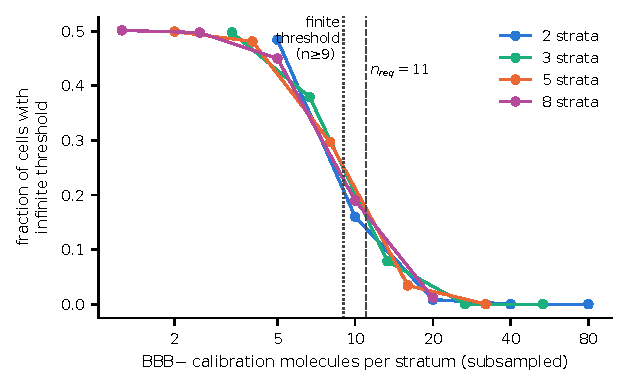
\includegraphics[width=0.62\linewidth]{supp_feasibility.pdf}\\[0.6em]
{\small% GENERATED by scripts/make_paper_numbers.py
\begin{tabular}{rcccc}
\toprule
\bbbm\ calibration size & 2 bins & 3 bins & 5 bins & 8 bins\\
\midrule
10 & 0.484 (5.0) & 0.498 (3.3) & 0.499 (2.0) & 0.501 (1.2)\\
20 & 0.160 (10.0) & 0.379 (6.7) & 0.481 (4.0) & 0.498 (2.5)\\
40 & 0.008 (20.0) & 0.079 (13.3) & 0.297 (8.0) & 0.450 (5.0)\\
80 & 0.000 (40.0) & 0.000 (26.7) & 0.034 (16.0) & 0.190 (10.0)\\
160 & 0.000 (80.0) & 0.000 (53.3) & 0.000 (32.0) & 0.012 (20.0)\\
realized (\V{cg.ncalmin.min}--\V{cg.ncalmin.max}) & 0.000 & 0.006 & 0.065 & 0.154\\
\bottomrule
\end{tabular}
}
\caption{\textbf{Feasibility of fixed class $\times$ support partitions} against minority calibration molecules per stratum (BBB$-$ calibration subsampled, 10 draws per split, majority retained; LAC, $\alpha=0.1$, CE; mean over setting $\times$ backbone cells in which the size is reachable in all 20 splits). Dotted: finite-threshold condition; dashed: $\nreq=11$. Table: the plotted values; parentheses, BBB$-$ calibration molecules per stratum; last row, the realized calibration sets without subsampling.}\label{fig:feas}
\end{figure}

\subsection{Exact invariances}
\begin{proposition}[Invariance to post-hoc per-class recalibration]\label{prop:S-inv}
If $\hat p'_y=h_y(\hat p_y)$ with each $h_y$ strictly increasing, class-conditional and class $\times$ support LAC prediction sets are unchanged; marginal LAC sets are in general changed.
\end{proposition}
\begin{proof}
Within class $y$, all calibration and test LAC scores are transformed by the same strictly increasing map $u\mapsto1-h_y(1-u)$, which preserves their order. Each per-class or per-cell threshold is an order statistic of class-$y$ scores, and membership is the comparison $s(x,y)\le\hat q_y$, which the common map preserves. A marginal threshold is an order statistic of scores of both classes, transformed by different maps, so the ordering between classes, and hence the threshold, can change.
\end{proof}
\noindent\textbf{Remark.} For a binary model, temperature scaling applies the same increasing map to the logit of both classes, so $h_1(p)=1-h_0(1-p)$ and both classes' LAC scores share one map; marginal sets are then unchanged as well. Logit adjustment shifts the two classes differently. Empirically (Stage B rows, 12 in-domain cells), temperature scaling and logit adjustment change class-conditional, class $\times$ support and merged sets by at most \V{inv.ts.max} and \V{inv.la.max} in any endpoint, the nonzero value being a set-size difference caused by ties among probabilities stored in single precision near 1; marginal sets change by at most \V{inv.marginal_ts.max} under temperature scaling and by up to \V{inv.marginal_la.cov} in BBB$-$ coverage and \V{inv.marginal_la.low} in low-support BBB$-$ coverage under logit adjustment.

\begin{proposition}[Margin and LAC coincide for binary tasks]\label{prop:S-margin}
For $K=2$, the margin score $\max_{y'\neq y}\hat p_{y'}-\hat p_y=1-2\hat p_y=2s_{\mathrm{LAC}}(x,y)-1$, a strictly increasing affine function of LAC common to both labels; every calibrator whose threshold is an order statistic of scores therefore returns identical sets.
\end{proposition}

\subsection{Exact results versus design choices, and relation to prior theory}
\begin{table}[h]\centering\small
\caption{\textbf{Status of each formal statement.}}\label{tab:exact}
\begin{tabular}{p{0.36\linewidth}p{0.2\linewidth}p{0.34\linewidth}}\toprule
Statement & Status & Scope\\\midrule
Stratum floor (Prop.~\ref{prop:S-floor}) & exact & any class-conditionally valid predictor\\
Shared-threshold coverage (Prop.~\ref{prop:S-shared}) & exact & I, C; ordering needs stochastic dominance\\
Cell coverage band (Prop.~\ref{prop:S-band}) & exact & fixed partition; E, C\\
Cell-size change (Cor.~\ref{cor:S-cell}) & exact two-sided bound & class level; random strata\\
Merging validity (Thm.~\ref{thm:S}) & exact & realized merged groups; E\\
Beta law & exact~\cite{vovk2012conditional} & i.i.d., continuous scores; over calibration draws\\
$\nreq$ and $B\le n^{-}_{\mathrm{cal}}/\nreq$ & design choice & tolerance $\epsilon=\alpha$, $\delta=0.1$; heuristic\\
Invariances (Props.~\ref{prop:S-inv}, \ref{prop:S-margin}) & exact & LAC; binary for the margin\\\bottomrule
\end{tabular}\end{table}
No informative method can guarantee distribution-free coverage conditional on every subgroup~\cite{barber2021limits}, so practical methods condition on a finite taxonomy, and a subgroup outside it can be under-covered. That result does not identify the subgroup or the direction. Proposition~\ref{prop:S-shared} does so when scores are stochastically ordered across strata: the stratum with stochastically largest scores is the under-covered one. In these data a pre-assay covariate (support) identifies the under-covered subgroup, and Proposition~\ref{prop:S-band} shows that joint conditioning on it removes the gradient at a cost bounded cell by cell. Clustered~\cite{ding2023clustered}, Kandinsky~\cite{bairaktari2025kandinsky}, interpolated~\cite{ding2026longtail}, localized~\cite{guan2023lcp,hore2025rlcp} and function-class-conditional~\cite{gibbs2025conditional} methods choose or relax the taxonomy differently; Section~\ref{sec:mech} compares them on the same predictions.

% =====================================================================
\section{Data, splits and models}\label{sec:data}
\textbf{Curation.} SMILES were standardized (largest organic fragment, neutralization, canonical isomeric SMILES), de-duplicated by InChIKey with conflicting-label groups removed, and stereoisomer families sharing a connectivity key collapsed to one record when labels agreed and removed otherwise. This gives \V{data.bbbp.n} BBBP molecules (\V{data.bbbp.minfrac}\% BBB$-$) and \V{data.b3db.n} B3DB molecules (\V{data.b3db.minfrac}\% BBB$-$). The external transfer set contains the \V{data.transfer.n} B3DB molecules whose connectivity key does not occur in BBBP (\V{data.transfer.nmin} BBB$-$).

\textbf{Splits.} TRAIN/VAL/CAL/TEST fractions are 60/10/15/15\%. Random splits permute molecules uniformly. Balanced scaffold splits assign Bemis-Murcko scaffold groups at random, with large groups placed in TRAIN and acyclic molecules treated as singleton groups. Cluster holdout withholds whole $k$-means clusters of ECFP4 fingerprints ($k=20$) as TEST. Transfer trains and calibrates on BBBP scaffold splits and tests on the external set. No split function receives labels.

\textbf{Support.} $s_{\max}$ is the maximal Tanimoto similarity of 2048-bit ECFP4 fingerprints (radius 2) to TRAIN, computed per split for VAL, CAL and TEST. Stratum edges are VAL quantiles. The CAL-edge variant is reported in Table~\ref{tab:rs}.

\textbf{Models.} Random forest: 500 trees, $\sqrt{d}$ features, ECFP4 input. GIN: 5 layers, 128 hidden units, dropout 0.5, learning rate $10^{-3}$, weight decay $10^{-5}$, up to 60 epochs with patience 15 on VAL AUROC. Chemprop v2 D-MPNN: default bond message passing, mean aggregation, batch normalization, up to 40 epochs with patience 10 on VAL loss. wCE uses inverse class-frequency weights.

\textbf{Predictive performance.} Table~\ref{tab:perf} reports the held-out discrimination of each backbone, so that the coverage results can be read against model competence.

\begin{table}[h]\centering\scriptsize
\caption{\textbf{Predictive performance on TEST} (mean and SD over 20 splits, CE). AUPRC and recall refer to the BBB$-$ class; balanced accuracy and recall use the argmax decision.}\label{tab:perf}
\resizebox{\linewidth}{!}{% GENERATED by scripts/make_supplement_tables.py
\begin{tabular}{llccccc}
\toprule
Setting & Model & AUROC (SD) & AUPRC, BBB$-$ (SD) & BBB$-$ share & balanced acc. & BBB$-$ recall\\
\midrule
BBBP random & RF & 0.911 (0.025) & 0.817 (0.049) & 0.24 & 0.795 & 0.615\\
BBBP random & GIN & 0.897 (0.023) & 0.780 (0.040) & 0.24 & 0.798 & 0.657\\
BBBP random & Chemprop & 0.910 (0.024) & 0.791 (0.045) & 0.24 & 0.813 & 0.688\\
BBBP scaffold & RF & 0.882 (0.037) & 0.773 (0.068) & 0.25 & 0.734 & 0.490\\
BBBP scaffold & GIN & 0.864 (0.057) & 0.746 (0.079) & 0.25 & 0.756 & 0.583\\
BBBP scaffold & Chemprop & 0.869 (0.038) & 0.728 (0.068) & 0.25 & 0.741 & 0.545\\
B3DB random & RF & 0.883 (0.011) & 0.817 (0.020) & 0.36 & 0.745 & 0.568\\
B3DB random & GIN & 0.861 (0.018) & 0.798 (0.027) & 0.36 & 0.757 & 0.631\\
B3DB random & Chemprop & 0.860 (0.015) & 0.792 (0.026) & 0.36 & 0.755 & 0.636\\
B3DB scaffold & RF & 0.867 (0.021) & 0.803 (0.029) & 0.37 & 0.729 & 0.539\\
B3DB scaffold & GIN & 0.846 (0.026) & 0.790 (0.031) & 0.37 & 0.743 & 0.615\\
B3DB scaffold & Chemprop & 0.843 (0.037) & 0.771 (0.050) & 0.37 & 0.738 & 0.627\\
BBBP$\to$B3DB & RF & 0.717 (0.008) & 0.728 (0.007) & 0.50 & 0.579 & 0.190\\
BBBP$\to$B3DB & GIN & 0.647 (0.020) & 0.678 (0.021) & 0.50 & 0.598 & 0.348\\
BBBP$\to$B3DB & Chemprop & 0.686 (0.014) & 0.688 (0.016) & 0.50 & 0.597 & 0.299\\
\bottomrule
\end{tabular}
}
\end{table}

\textbf{Pre-specification.} The primary family (endpoint, operating point, settings, backbones, three contrasts, Holm over 36) was fixed in a dated amendment to the statistical analysis plan on 21 October 2026, before the confirmatory Stage B outputs were analysed; $\nreq$ was frozen on 9 October 2026, before the confirmatory seeds were run.

% =====================================================================
\section{Additional results}\label{sec:more}
\textbf{Construction of main-text Figure 1.} The figure is generated by \path{scripts/make_fig1_overview.py} as an editable diagrams.net file from the confirmatory caches, and every value it shows is recomputed by the independent verifier. \emph{Setting.} For each of the twelve setting $\times$ backbone cells we took the mean high-minus-low BBB$-$ coverage gap under class-conditional calibration (LAC, $\alpha=0.1$, CE; \V{fig1.sel.gap12.low}--\V{fig1.sel.gap12.high}) and selected the lower median among the six random-split cells, where exchangeability holds and the panels can be read against Section~\ref{sec:proofs}: \V{fig1.sel.label}, gap \V{fig1.sel.gap}. The lower median of all twelve cells, \V{fig1.all12.label} (gap \V{fig1.sel.all12.gap}), lies in BBBP scaffold, the one setting in which the primary repair is not significant, so it would illustrate a correction that the paper does not claim. The rule was fixed after the confirmatory results were known; the figure is an illustration, not additional evidence. \emph{Panel B.} Each BBB$-$ test appearance is shown as its score minus the class-conditional threshold of its own split, so that zero is the applicable threshold for every point; no single raw threshold is drawn across splits, and the vertical axis spans the full range 0 to 1. The \V{fig1.B.n.low}, \V{fig1.B.n.mid} and \V{fig1.B.n.high} low-, mid- and high-support appearances come from \V{fig1.B.nmol.low}, \V{fig1.B.nmol.mid} and \V{fig1.B.nmol.high} distinct molecules; they are not independent, and the pooled curves are descriptive only (all inference in the paper is over splits). Of the pooled appearances, \V{fig1.B.excl.low}\%, \V{fig1.B.excl.mid}\% and \V{fig1.B.excl.high}\% lie above the threshold; one minus split-mean coverage in panel A gives \V{fig1.A.excl.low}\%, \V{fig1.A.excl.mid}\% and \V{fig1.A.excl.high}\%. The two differ by at most 0.1 percentage point, because pooling weights each split by its number of test appearances, and agree at the whole-percent precision printed in the panel. The panel restates the coverage arithmetic of Proposition~\ref{prop:S-shared} on these data; it does not identify why low-support compounds receive higher scores. Measured from the class threshold, the low-support class $\times$ support threshold lies between \V{fig1.B.shift.low.min} and \V{fig1.B.shift.low.max} and the high-support one between \V{fig1.B.shift.high.min} and \V{fig1.B.shift.high.max}; the low stratum has \V{fig1.B.ncal.low.min}--\V{fig1.B.ncal.low.max} BBB$-$ calibration compounds per split. Switching to class $\times$ support calibration covers \V{fig1.B.rescued} BBB$-$ test appearances that class-conditional calibration excluded (\V{fig1.B.rescued.low} low, \V{fig1.B.rescued.mid} mid, \V{fig1.B.rescued.high} high support) and excludes \V{fig1.B.lost} that it covered (\V{fig1.B.lost.low} low, \V{fig1.B.lost.mid} mid, \V{fig1.B.lost.high} high), the redistribution of Propositions~\ref{prop:S-shared} and~\ref{prop:S-band} seen in individual compounds. \emph{Example pair.} Among BBB$-$ test compounds in the low-support tertile at every appearance, we took the one with the most splits in which it is excluded under class-conditional and included under class $\times$ support calibration (ties: more appearances, then identifier). This is halofantrine: our identifier \V{fig1.mol.id}, B3DB record \V{fig1.mol.no} (``halofantrine hydrochloride'', PubChem CID \V{fig1.mol.cid}, BBB$-$, evidence group C, \V{fig1.mol.nref} reference), absent from BBBP. It is excluded and then included in \V{fig1.mol.rescued} of its \V{fig1.mol.n} test appearances, with maximal similarity to TRAIN \V{fig1.mol.smax.min}--\V{fig1.mol.smax.max} in all of them. In split \V{fig1.mol.seed}, the first such split, its BBB$-$ score is \V{fig1.mol.score} against a class threshold of \V{fig1.mol.qclass} (difference \V{fig1.mol.excess}) and a low-support threshold of \V{fig1.mol.qstratum}, set by \V{fig1.mol.ncal} BBB$-$ calibration compounds. Its most similar TRAIN compound in that split is B3DB record \V{fig1.nn.no}, 4-chlorobenzotrifluoride (our \V{fig1.mol.nn_id}, CID \V{fig1.nn.cid}, BBB$+$), at Tanimoto \V{fig1.mol.smax} on RDKit Morgan fingerprints of radius 2 and 2048 bits, the fingerprint that defines support; the next most similar TRAIN compound is at \V{fig1.nn.sim2}. The pair is drawn in the design strip with native bonds and atom labels from RDKit 2D coordinates. Halofantrine is not marked in panel B, because a point \V{fig1.mol.excess} from the threshold would be visually indistinguishable from the threshold itself.

\begin{table}[h]\centering\scriptsize
\caption{\textbf{Per-cell coverage with 95\% intervals over 20 splits} (LAC, $\alpha=0.1$, CE). $n^{-}_{\mathrm{cal}}$, $n^{-}_{\mathrm{test}}$, $n^{-}_{\mathrm{low}}$: mean BBB$-$ calibration, test and low-support test counts per split. C$\times$S: class $\times$ support.}\label{tab:cells}
\resizebox{\linewidth}{!}{% GENERATED by scripts/make_supplement_tables.py
\begin{tabular}{llrrrcccc}
\toprule
Setting & Model & $n^{-}_{\mathrm{cal}}$ & $n^{-}_{\mathrm{test}}$ & $n^{-}_{\mathrm{low}}$ & Mondrian low & Mondrian high & C$\times$S low & C$\times$S high\\
\midrule
BBBP random & RF & 65 & 70 & 19 & 0.79 [0.74, 0.84] & 0.94 [0.92, 0.96] & 0.93 [0.89, 0.96] & 0.89 [0.85, 0.93]\\
BBBP random & GIN & 65 & 70 & 19 & 0.81 [0.74, 0.87] & 0.95 [0.93, 0.97] & 0.93 [0.90, 0.97] & 0.91 [0.88, 0.94]\\
BBBP random & Chemprop & 65 & 70 & 19 & 0.84 [0.78, 0.90] & 0.97 [0.96, 0.98] & 0.96 [0.93, 0.99] & 0.91 [0.87, 0.95]\\
BBBP scaffold & RF & 67 & 72 & 25 & 0.82 [0.76, 0.87] & 0.96 [0.94, 0.98] & 0.91 [0.87, 0.95] & 0.92 [0.87, 0.96]\\
BBBP scaffold & GIN & 67 & 72 & 25 & 0.84 [0.78, 0.90] & 0.96 [0.92, 0.99] & 0.92 [0.87, 0.97] & 0.85 [0.77, 0.94]\\
BBBP scaffold & Chemprop & 67 & 72 & 25 & 0.85 [0.79, 0.91] & 0.97 [0.95, 0.99] & 0.94 [0.90, 0.97] & 0.88 [0.81, 0.95]\\
B3DB random & RF & 210 & 210 & 73 & 0.87 [0.85, 0.89] & 0.94 [0.93, 0.96] & 0.93 [0.91, 0.94] & 0.91 [0.89, 0.94]\\
B3DB random & GIN & 210 & 210 & 73 & 0.86 [0.83, 0.88] & 0.96 [0.94, 0.97] & 0.92 [0.90, 0.94] & 0.92 [0.90, 0.94]\\
B3DB random & Chemprop & 210 & 210 & 73 & 0.85 [0.83, 0.87] & 0.96 [0.95, 0.98] & 0.91 [0.90, 0.93] & 0.90 [0.88, 0.92]\\
B3DB scaffold & RF & 221 & 216 & 79 & 0.84 [0.82, 0.87] & 0.94 [0.92, 0.96] & 0.90 [0.88, 0.92] & 0.89 [0.86, 0.92]\\
B3DB scaffold & GIN & 221 & 216 & 79 & 0.83 [0.80, 0.87] & 0.94 [0.92, 0.96] & 0.88 [0.84, 0.92] & 0.89 [0.86, 0.92]\\
B3DB scaffold & Chemprop & 221 & 216 & 79 & 0.85 [0.82, 0.87] & 0.95 [0.93, 0.96] & 0.89 [0.87, 0.92] & 0.91 [0.88, 0.93]\\
\bottomrule
\end{tabular}
}
\end{table}

\begin{table}[h]\centering\scriptsize
\caption{\textbf{Pre-specified primary family} (36 tests). $\Delta$: mean paired difference in low-support BBB$-$ coverage; seed CI: bootstrap over splits; $p$: Wilcoxon signed-rank; Holm$_{36}$: Holm-adjusted over the 36 tests. Molecule CI and Holm$_{\mathrm{mol}}$, Holm$_{\mathrm{scaf}}$: bootstrap over unique test molecules or scaffolds (\V{boot.B} draws, calibration fixed), Holm over 36.}\label{tab:primary}
\resizebox{\linewidth}{!}{% GENERATED by scripts/make_supplement_tables.py
\begin{tabular}{lllrcccccc}
\toprule
Setting & Model & Contrast & $\Delta$ & Seed CI & $p$ & Holm$_{36}$ & Molecule CI & Holm$_{\mathrm{mol}}$ & Holm$_{\mathrm{scaf}}$\\
\midrule
B3DB random & Chemprop & C$\times$S - Mondrian & +0.066 & [0.050, 0.084] & $<$0.001 & 0.004 & [0.052, 0.081] & 0.004 & 0.004\\
B3DB random & Chemprop & SABM - Mondrian & +0.066 & [0.050, 0.084] & $<$0.001 & 0.004 & [0.052, 0.081] & 0.004 & 0.004\\
B3DB random & Chemprop & SABM - C$\times$S & +0.000 & [0.000, 0.000] & 1.000 & 1.000 & [0.000, 0.000] & 1.000 & 1.000\\
B3DB random & GIN & C$\times$S - Mondrian & +0.063 & [0.050, 0.077] & $<$0.001 & $<$0.001 & [0.050, 0.078] & 0.004 & 0.004\\
B3DB random & GIN & SABM - Mondrian & +0.063 & [0.050, 0.077] & $<$0.001 & $<$0.001 & [0.050, 0.078] & 0.004 & 0.004\\
B3DB random & GIN & SABM - C$\times$S & +0.000 & [0.000, 0.000] & 1.000 & 1.000 & [0.000, 0.000] & 1.000 & 1.000\\
B3DB random & RF & C$\times$S - Mondrian & +0.059 & [0.039, 0.080] & $<$0.001 & 0.004 & [0.045, 0.074] & 0.004 & 0.004\\
B3DB random & RF & SABM - Mondrian & +0.059 & [0.039, 0.080] & $<$0.001 & 0.004 & [0.045, 0.074] & 0.004 & 0.004\\
B3DB random & RF & SABM - C$\times$S & +0.000 & [0.000, 0.000] & 1.000 & 1.000 & [0.000, 0.000] & 1.000 & 1.000\\
B3DB scaffold & Chemprop & C$\times$S - Mondrian & +0.048 & [0.032, 0.066] & $<$0.001 & 0.004 & [0.037, 0.059] & 0.004 & 0.004\\
B3DB scaffold & Chemprop & SABM - Mondrian & +0.048 & [0.032, 0.066] & $<$0.001 & 0.004 & [0.037, 0.059] & 0.004 & 0.004\\
B3DB scaffold & Chemprop & SABM - C$\times$S & +0.000 & [0.000, 0.000] & 1.000 & 1.000 & [0.000, 0.000] & 1.000 & 1.000\\
B3DB scaffold & GIN & C$\times$S - Mondrian & +0.045 & [0.028, 0.062] & $<$0.001 & 0.012 & [0.035, 0.057] & 0.004 & 0.004\\
B3DB scaffold & GIN & SABM - Mondrian & +0.045 & [0.028, 0.062] & $<$0.001 & 0.012 & [0.035, 0.057] & 0.004 & 0.004\\
B3DB scaffold & GIN & SABM - C$\times$S & +0.000 & [0.000, 0.000] & 1.000 & 1.000 & [0.000, 0.000] & 1.000 & 1.000\\
B3DB scaffold & RF & C$\times$S - Mondrian & +0.054 & [0.036, 0.076] & $<$0.001 & 0.005 & [0.042, 0.067] & 0.004 & 0.004\\
B3DB scaffold & RF & SABM - Mondrian & +0.054 & [0.036, 0.076] & $<$0.001 & 0.005 & [0.042, 0.067] & 0.004 & 0.004\\
B3DB scaffold & RF & SABM - C$\times$S & +0.000 & [0.000, 0.000] & 1.000 & 1.000 & [0.000, 0.000] & 1.000 & 1.000\\
BBBP random & Chemprop & C$\times$S - Mondrian & +0.120 & [0.074, 0.168] & $<$0.001 & 0.006 & [0.082, 0.161] & 0.004 & 0.004\\
BBBP random & Chemprop & SABM - Mondrian & +0.120 & [0.074, 0.168] & $<$0.001 & 0.006 & [0.082, 0.161] & 0.004 & 0.004\\
BBBP random & Chemprop & SABM - C$\times$S & +0.000 & [0.000, 0.000] & 1.000 & 1.000 & [0.000, 0.000] & 1.000 & 1.000\\
BBBP random & GIN & C$\times$S - Mondrian & +0.126 & [0.082, 0.173] & $<$0.001 & 0.005 & [0.087, 0.168] & 0.004 & 0.004\\
BBBP random & GIN & SABM - Mondrian & +0.126 & [0.082, 0.173] & $<$0.001 & 0.005 & [0.087, 0.168] & 0.004 & 0.004\\
BBBP random & GIN & SABM - C$\times$S & +0.000 & [0.000, 0.000] & 1.000 & 1.000 & [0.000, 0.000] & 1.000 & 1.000\\
BBBP random & RF & C$\times$S - Mondrian & +0.137 & [0.089, 0.187] & $<$0.001 & 0.005 & [0.096, 0.181] & 0.004 & 0.004\\
BBBP random & RF & SABM - Mondrian & +0.137 & [0.089, 0.187] & $<$0.001 & 0.005 & [0.096, 0.181] & 0.004 & 0.004\\
BBBP random & RF & SABM - C$\times$S & +0.000 & [0.000, 0.000] & 1.000 & 1.000 & [0.000, 0.000] & 1.000 & 1.000\\
BBBP scaffold & Chemprop & C$\times$S - Mondrian & +0.083 & [0.032, 0.141] & 0.005 & 0.077 & [0.053, 0.116] & 0.004 & 0.004\\
BBBP scaffold & Chemprop & SABM - Mondrian & +0.083 & [0.032, 0.141] & 0.005 & 0.077 & [0.053, 0.116] & 0.004 & 0.004\\
BBBP scaffold & Chemprop & SABM - C$\times$S & +0.000 & [0.000, 0.000] & 1.000 & 1.000 & [0.000, 0.000] & 1.000 & 1.000\\
BBBP scaffold & GIN & C$\times$S - Mondrian & +0.082 & [0.032, 0.137] & 0.004 & 0.077 & [0.053, 0.113] & 0.004 & 0.004\\
BBBP scaffold & GIN & SABM - Mondrian & +0.082 & [0.032, 0.137] & 0.004 & 0.077 & [0.053, 0.113] & 0.004 & 0.004\\
BBBP scaffold & GIN & SABM - C$\times$S & +0.000 & [0.000, 0.000] & 1.000 & 1.000 & [0.000, 0.000] & 1.000 & 1.000\\
BBBP scaffold & RF & C$\times$S - Mondrian & +0.091 & [0.042, 0.143] & 0.004 & 0.077 & [0.063, 0.121] & 0.004 & 0.004\\
BBBP scaffold & RF & SABM - Mondrian & +0.091 & [0.042, 0.143] & 0.004 & 0.077 & [0.063, 0.121] & 0.004 & 0.004\\
BBBP scaffold & RF & SABM - C$\times$S & +0.000 & [0.000, 0.000] & 1.000 & 1.000 & [0.000, 0.000] & 1.000 & 1.000\\
\bottomrule
\end{tabular}
}
\end{table}

\begin{table}[h]\centering\scriptsize
\caption{\textbf{Empirical settings} (LAC, $\alpha=0.1$, CE; mean over 20 splits). No finite-sample guarantee applies.}\label{tab:shift}
\resizebox{\linewidth}{!}{% GENERATED by scripts/make_supplement_tables.py
\begin{tabular}{llcccccccc}
\toprule
Setting & Model & Marg.\ BBB$-$ & Mond.\ BBB$-$ & Marg.\ BBB$+$ & Mond.\ BBB$+$ & Mond.\ low & C$\times$S low & Size M & Size C$\times$S\\
\midrule
BBBP$\to$B3DB & RF & 0.38 & 0.86 & 0.98 & 0.77 & 0.84 & 0.90 & 1.36 & 1.45\\
BBBP$\to$B3DB & GIN & 0.50 & 0.77 & 0.92 & 0.81 & 0.74 & 0.88 & 1.41 & 1.51\\
BBBP$\to$B3DB & Chemprop & 0.51 & 0.81 & 0.95 & 0.79 & 0.78 & 0.88 & 1.36 & 1.46\\
BBBP cluster & RF & 0.54 & 0.92 & 0.99 & 0.79 & 0.94 & 0.98 & 1.33 & 1.46\\
BBBP cluster & GIN & 0.69 & 0.82 & 0.93 & 0.83 & 0.84 & 0.93 & 1.25 & 1.38\\
BBBP cluster & Chemprop & 0.65 & 0.84 & 0.93 & 0.84 & 0.85 & 0.89 & 1.26 & 1.36\\
B3DB cluster & RF & 0.74 & 0.92 & 0.98 & 0.79 & 0.92 & 0.95 & 1.45 & 1.52\\
B3DB cluster & GIN & 0.74 & 0.83 & 0.93 & 0.87 & 0.81 & 0.86 & 1.38 & 1.48\\
B3DB cluster & Chemprop & 0.74 & 0.84 & 0.92 & 0.85 & 0.83 & 0.89 & 1.36 & 1.48\\
\bottomrule
\end{tabular}
}
\end{table}

\begin{table}[h]\centering\scriptsize
\caption{\textbf{Score and level sensitivity.} Low-support BBB$-$ coverage, mean (range) over the 12 in-domain cells (six random-split and six scaffold-split), CE.}\label{tab:rsc}
% GENERATED by scripts/make_supplement_tables.py
\begin{tabular}{lccc}
\toprule
Score, level & Mondrian low & C$\times$S low & cells with gain $>0$\\
\midrule
LAC, $\alpha=0.10$ (primary) & 0.837 (0.79--0.87) & 0.918 (0.88--0.96) & 12/12\\
APS, $\alpha=0.10$ & 0.847 (0.82--0.88) & 0.915 (0.89--0.95) & 12/12\\
RAPS, $\alpha=0.10$ & 0.852 (0.81--0.87) & 0.918 (0.88--0.95) & 12/12\\
LAC, $\alpha=0.05$ & 0.928 (0.91--0.95) & 0.967 (0.94--0.99) & 12/12\\
LAC, $\alpha=0.20$ & 0.687 (0.59--0.75) & 0.816 (0.76--0.88) & 12/12\\
\bottomrule
\end{tabular}

\end{table}

\begin{table}[h]\centering\scriptsize
\caption{\textbf{Second Mondrian dimension.} Low-support BBB$-$ coverage evaluated on the common VAL tertiles and mean set size, over the 12 in-domain cells (six random-split and six scaffold-split) (LAC, $\alpha=0.1$, CE).}\label{tab:rs}
% GENERATED by scripts/make_supplement_tables.py
\begin{tabular}{lccc}
\toprule
Second Mondrian dimension & low-support BBB$-$ (mean) & range & set size\\
\midrule
class only (Mondrian) & 0.837 & 0.79--0.87 & 1.285\\
max-Tanimoto tertiles (primary) & 0.918 & 0.88--0.96 & 1.329\\
max-Tanimoto, 2 bins & 0.908 & 0.87--0.95 & 1.308\\
max-Tanimoto, 5 bins & 0.928 & 0.88--0.97 & 1.381\\
mean top-5 Tanimoto tertiles & 0.905 & 0.86--0.93 & 1.326\\
MACCS max-Tanimoto tertiles & 0.892 & 0.85--0.92 & 1.333\\
$k$-means clusters ($k=3$) & 0.855 & 0.83--0.88 & 1.390\\
TPSA strata ($<60$, 60--90, $>90$) & 0.868 & 0.84--0.89 & 1.501\\
tertile edges from CAL & 0.913 & 0.86--0.94 & 1.326\\
random strata (control) & 0.860 & 0.83--0.89 & 1.335\\
\bottomrule
\end{tabular}

\end{table}

\begin{table}[h]\centering\scriptsize
\caption{\textbf{Same-cell-size control} (exploratory). Low- and high-support BBB$-$ coverage under class-conditional calibration, class $\times$ randomly assigned strata of equal size, and class $\times$ Tanimoto tertiles (C$\times$S), with mean set sizes; paired difference in low-support coverage, seed bootstrap interval, and Holm-adjusted Wilcoxon $p$ over the 12 cells. LAC, $\alpha=0.1$, CE, 20 splits.}\label{tab:randstrata}
\resizebox{\linewidth}{!}{% GENERATED by scripts/make_supplement_tables.py
\begin{tabular}{llcccccc}
\toprule
Setting & Model & Mondrian low/high & random strata low/high & C$\times$S low/high & size rand./C$\times$S & C$\times$S $-$ random, low & Holm $p$\\
\midrule
B3DB random & Chemprop & 0.85 / 0.96 & 0.85 / 0.97 & 0.91 / 0.90 & 1.35 / 1.33 & +0.059 [0.043, 0.075] & 0.001\\
B3DB random & GIN & 0.86 / 0.96 & 0.86 / 0.96 & 0.92 / 0.92 & 1.35 / 1.35 & +0.055 [0.042, 0.069] & 0.001\\
B3DB random & RF & 0.87 / 0.94 & 0.89 / 0.95 & 0.93 / 0.91 & 1.28 / 1.29 & +0.043 [0.026, 0.060] & 0.005\\
B3DB scaffold & Chemprop & 0.85 / 0.95 & 0.86 / 0.95 & 0.89 / 0.91 & 1.35 / 1.35 & +0.036 [0.017, 0.054] & 0.014\\
B3DB scaffold & GIN & 0.83 / 0.94 & 0.84 / 0.94 & 0.88 / 0.89 & 1.35 / 1.35 & +0.037 [0.017, 0.056] & 0.013\\
B3DB scaffold & RF & 0.84 / 0.94 & 0.86 / 0.94 & 0.90 / 0.89 & 1.30 / 1.30 & +0.040 [0.022, 0.059] & 0.008\\
BBBP random & Chemprop & 0.84 / 0.97 & 0.88 / 0.98 & 0.96 / 0.91 & 1.32 / 1.29 & +0.084 [0.048, 0.123] & 0.004\\
BBBP random & GIN & 0.81 / 0.95 & 0.84 / 0.95 & 0.93 / 0.91 & 1.29 / 1.30 & +0.090 [0.050, 0.133] & 0.008\\
BBBP random & RF & 0.79 / 0.94 & 0.83 / 0.96 & 0.93 / 0.89 & 1.27 / 1.29 & +0.100 [0.061, 0.140] & 0.005\\
BBBP scaffold & Chemprop & 0.85 / 0.97 & 0.86 / 0.97 & 0.94 / 0.88 & 1.37 / 1.36 & +0.073 [0.029, 0.124] & 0.020\\
BBBP scaffold & GIN & 0.84 / 0.96 & 0.89 / 0.98 & 0.92 / 0.85 & 1.41 / 1.38 & +0.037 [-0.003, 0.075] & 0.059\\
BBBP scaffold & RF & 0.82 / 0.96 & 0.86 / 0.97 & 0.91 / 0.92 & 1.37 / 1.35 & +0.046 [-0.003, 0.097] & 0.099\\
\bottomrule
\end{tabular}
}
\end{table}

\begin{table}[h]\centering\scriptsize
\caption{\textbf{Common evaluation grid.} Every partition scored on the lowest VAL tertile (low-tertile cov.) and on the worst VAL sextile with at least five BBB$-$ molecules; BBB$-$ calibration subsampled (10 draws per split), majority retained; LAC, $\alpha=0.1$, CE. Cells: setting $\times$ backbone combinations reachable in all 20 splits. Degenerate: fraction of (class, stratum) cells with an infinite threshold.}\label{tab:grid}
\resizebox{\linewidth}{!}{% GENERATED by scripts/make_supplement_tables.py
\begin{tabular}{llrccccc}
\toprule
$n^{-}_{\mathrm{cal}}$ & Partition & cells & low-tertile cov. & worst sextile & set size & singleton & degenerate\\
\midrule
realized & mondrian & 12 & 0.837 & 0.764 & 1.285 & 0.715 & 0.000\\
realized & fixed-b2 & 12 & 0.908 & 0.783 & 1.308 & 0.688 & 0.000\\
realized & fixed-b3 & 12 & 0.918 & 0.787 & 1.329 & 0.662 & 0.006\\
realized & fixed-b5 & 12 & 0.928 & 0.817 & 1.381 & 0.611 & 0.065\\
realized & fixed-b8 & 12 & 0.940 & 0.833 & 1.471 & 0.520 & 0.154\\
realized & sabm-b3 & 12 & 0.918 & 0.788 & 1.324 & 0.668 & 0.000\\
realized & sabm-b8 & 12 & 0.923 & 0.796 & 1.374 & 0.616 & 0.000\\
\midrule
160 & mondrian & 6 & 0.849 & 0.798 & 1.310 & 0.690 & 0.000\\
160 & fixed-b2 & 6 & 0.896 & 0.809 & 1.325 & 0.675 & 0.000\\
160 & fixed-b3 & 6 & 0.905 & 0.809 & 1.334 & 0.664 & 0.000\\
160 & fixed-b5 & 6 & 0.912 & 0.824 & 1.359 & 0.638 & 0.000\\
160 & fixed-b8 & 6 & 0.921 & 0.832 & 1.401 & 0.596 & 0.012\\
160 & sabm-b3 & 6 & 0.905 & 0.809 & 1.334 & 0.664 & 0.000\\
160 & sabm-b8 & 6 & 0.920 & 0.830 & 1.392 & 0.604 & 0.000\\
\midrule
80 & mondrian & 6 & 0.851 & 0.801 & 1.315 & 0.685 & 0.000\\
80 & fixed-b2 & 6 & 0.902 & 0.809 & 1.340 & 0.660 & 0.000\\
80 & fixed-b3 & 6 & 0.914 & 0.812 & 1.361 & 0.636 & 0.000\\
80 & fixed-b5 & 6 & 0.925 & 0.833 & 1.419 & 0.577 & 0.034\\
80 & fixed-b8 & 6 & 0.940 & 0.848 & 1.523 & 0.473 & 0.190\\
80 & sabm-b3 & 6 & 0.914 & 0.813 & 1.361 & 0.636 & 0.000\\
80 & sabm-b8 & 6 & 0.924 & 0.819 & 1.402 & 0.594 & 0.000\\
\midrule
40 & mondrian & 12 & 0.832 & 0.760 & 1.289 & 0.711 & 0.000\\
40 & fixed-b2 & 12 & 0.924 & 0.795 & 1.354 & 0.640 & 0.008\\
40 & fixed-b3 & 12 & 0.935 & 0.807 & 1.419 & 0.573 & 0.079\\
40 & fixed-b5 & 12 & 0.959 & 0.860 & 1.568 & 0.424 & 0.297\\
40 & fixed-b8 & 12 & 0.987 & 0.945 & 1.703 & 0.293 & 0.450\\
40 & sabm-b3 & 12 & 0.921 & 0.792 & 1.357 & 0.637 & 0.000\\
40 & sabm-b8 & 12 & 0.922 & 0.803 & 1.396 & 0.597 & 0.000\\
\midrule
20 & mondrian & 12 & 0.839 & 0.771 & 1.311 & 0.688 & 0.000\\
20 & fixed-b2 & 12 & 0.944 & 0.829 & 1.466 & 0.526 & 0.160\\
20 & fixed-b3 & 12 & 0.975 & 0.897 & 1.628 & 0.366 & 0.379\\
20 & fixed-b5 & 12 & 0.996 & 0.984 & 1.724 & 0.274 & 0.481\\
20 & fixed-b8 & 12 & 0.999 & 0.995 & 1.754 & 0.245 & 0.498\\
20 & sabm-b3 & 12 & 0.839 & 0.771 & 1.317 & 0.681 & 0.000\\
20 & sabm-b8 & 12 & 0.839 & 0.771 & 1.336 & 0.662 & 0.000\\
\midrule
10 & mondrian & 12 & 0.845 & 0.783 & 1.338 & 0.659 & 0.000\\
10 & fixed-b2 & 12 & 0.997 & 0.989 & 1.720 & 0.280 & 0.484\\
10 & fixed-b3 & 12 & 1.000 & 0.997 & 1.737 & 0.263 & 0.498\\
10 & fixed-b5 & 12 & 1.000 & 1.000 & 1.745 & 0.255 & 0.499\\
10 & fixed-b8 & 12 & 1.000 & 1.000 & 1.760 & 0.240 & 0.501\\
10 & sabm-b3 & 12 & 0.845 & 0.783 & 1.344 & 0.652 & 0.000\\
10 & sabm-b8 & 12 & 0.845 & 0.783 & 1.363 & 0.633 & 0.000\\
\bottomrule
\end{tabular}
}
\end{table}

\begin{table}[h]\centering\scriptsize
\caption{\textbf{Training loss.} Marginal BBB$-$ coverage, class-conditional low-support coverage and class-conditional set size under CE and wCE (LAC, $\alpha=0.1$).}\label{tab:loss}
% GENERATED by scripts/make_supplement_tables.py
\begin{tabular}{llcccccc}
\toprule
Setting & Model & Marg.\ CE & Marg.\ wCE & Mond.\ low CE & Mond.\ low wCE & Size CE & Size wCE\\
\midrule
BBBP random & RF & 0.65 & 0.65 & 0.79 & 0.83 & 1.17 & 1.16\\
BBBP random & GIN & 0.72 & 0.89 & 0.81 & 0.81 & 1.23 & 1.26\\
BBBP random & Chemprop & 0.75 & 0.80 & 0.84 & 0.84 & 1.23 & 1.21\\
BBBP scaffold & RF & 0.62 & 0.62 & 0.82 & 0.82 & 1.28 & 1.27\\
BBBP scaffold & GIN & 0.69 & 0.87 & 0.84 & 0.86 & 1.34 & 1.35\\
BBBP scaffold & Chemprop & 0.71 & 0.75 & 0.85 & 0.85 & 1.32 & 1.32\\
B3DB random & RF & 0.79 & 0.79 & 0.87 & 0.87 & 1.26 & 1.27\\
B3DB random & GIN & 0.82 & 0.90 & 0.86 & 0.85 & 1.33 & 1.32\\
B3DB random & Chemprop & 0.81 & 0.85 & 0.85 & 0.87 & 1.32 & 1.33\\
B3DB scaffold & RF & 0.77 & 0.77 & 0.84 & 0.84 & 1.29 & 1.29\\
B3DB scaffold & GIN & 0.81 & 0.86 & 0.83 & 0.83 & 1.33 & 1.32\\
B3DB scaffold & Chemprop & 0.82 & 0.85 & 0.85 & 0.86 & 1.33 & 1.36\\
\bottomrule
\end{tabular}

\end{table}

% =====================================================================
\section{Mechanism and existing conditional methods (exploratory)}\label{sec:mech}
\textbf{Existing methods.} Table~\ref{tab:condbase} evaluates published conditional, localized and reweighted conformal methods on the cached predictions of the 12 in-domain cells (six random-split and six scaffold-split). Several are our own implementations or approximations of the published ideas, as stated in the table; they are included to test whether the support gradient survives methods designed for conditional coverage, not to rank those methods.

\begin{table}[h]\centering\scriptsize
\caption{\textbf{Existing conditional conformal methods} on the same predictions (LAC, $\alpha=0.1$, CE; 12 in-domain cells (six random-split and six scaffold-split), 20 splits each). Low-support BBB$-$: range over cells of the seed-mean coverage in the lowest VAL Tanimoto tertile; high: mean over cells for the highest tertile; cells failing: cells whose 95\% interval for low-support coverage lies below 0.90; set size: mean over cells.}\label{tab:condbase}
\resizebox{\linewidth}{!}{% GENERATED by scripts/make_supplement_tables.py
\begin{tabular}{p{4.4cm}p{3.6cm}cccc}
\toprule
Method & Implementation & low-support BBB$-$ & high & cells failing & set size\\
\midrule
marginal split CP & standard & 0.30--0.76 & 0.87 & 12 & 1.19\\
class-conditional (Mondrian) & standard & 0.79--0.87 & 0.95 & 10 & 1.29\\
class x support, fixed tertiles & standard Mondrian taxonomy & 0.88--0.96 & 0.90 & 0 & 1.33\\
Mondrian, training-conditional (PAC) & Vovk 2012 rank rule & 0.86--0.92 & 0.97 & 1 & 1.40\\
Mondrian, SSBC-style Beta rank & our implementation & 0.86--0.92 & 0.97 & 1 & 1.40\\
clustered CP over class x support cells & our implementation of Ding et al. 2023 & 0.68--0.89 & 0.84 & 8 & 1.25\\
Kandinsky-style group QR & our approximation, not the authors' algorithm & 0.89--0.95 & 0.92 & 0 & 1.47\\
conditional QR on support & our approximation of Gibbs et al. 2025 & 0.88--0.94 & 0.91 & 0 & 1.33\\
INTERP-Q (q=0.5) & our implementation of Ding et al. 2026 & 0.52--0.81 & 0.91 & 12 & 1.22\\
INTERP-Q (q=0.9) & our implementation of Ding et al. 2026 & 0.73--0.85 & 0.95 & 12 & 1.26\\
RC3P & our implementation & 0.79--0.87 & 0.95 & 10 & 1.31\\
localized CP, Tanimoto kernel & our implementation of Guan 2023 & 0.86--0.98 & 0.97 & 1 & 1.47\\
localized CP, kNN & our implementation & 0.80--0.89 & 0.95 & 8 & 1.33\\
randomly localized CP & our implementation of Hore and Barber 2025 & 0.86--0.94 & 0.92 & 1 & 1.32\\
weighted Mondrian (density ratio) & our approximation & 0.78--0.91 & 0.96 & 7 & 1.34\\
KMM-weighted Mondrian & our approximation, not released KMM-CP & 0.76--0.87 & 0.95 & 11 & 1.28\\
macro-coverage CP & our implementation & 0.62--0.80 & 0.92 & 12 & 1.31\\
\bottomrule
\end{tabular}
}
\end{table}

\textbf{Mechanism.} For every split, the mean predicted probability of the true class was computed by support tertile, separately for BBB$-$ and BBB$+$ test compounds (Table~\ref{tab:mech}). Three predictions were stated before the confirmatory seeds were examined: (P1) low-support BBB$+$ compounds are covered at target while low-support BBB$-$ compounds are not; (P2) the true-class probability falls with support more for BBB$-$ than for BBB$+$; (P3) in the low-support tertile, the mean predicted BBB$-$ probability is below the observed BBB$-$ fraction. P2 holds in \V{mech.p2.n} of 12 cells. P1 fails: low-support BBB$+$ coverage is \V{mech.covmajlow.min}--\V{mech.covmajlow.max}, and the lower end of its 95\% interval is at or above 0.88 (a tolerance of 0.02 below target, fixed in advance) in \V{mech.p1.nmajok} of 12 cells. P3 holds in \V{mech.p3.n} of 12 cells (\V{mech.p3.nb3db} of 6 on B3DB).

\begin{table}[h]\centering\scriptsize
\caption{\textbf{True-class probability and coverage by support} under class-conditional calibration (LAC, $\alpha=0.1$, CE; 20 splits). $\bar p_{\mathrm{true}}$: mean predicted probability of the true class in the highest and lowest support tertile; cov.: low-support coverage of minority and majority compounds; calib.\ gap: mean predicted minority probability minus observed minority fraction in the lowest tertile, with 95\% interval. Lower block: random forest on the additional tasks (Section~\ref{sec:general}).}\label{tab:mech}
\resizebox{\linewidth}{!}{% GENERATED by scripts/make_supplement_tables.py
\begin{tabular}{llccccc}
\toprule
Setting & Model & $\bar p_{\mathrm{true}}$ minority, high$\to$low & $\bar p_{\mathrm{true}}$ majority, high$\to$low & cov.\ min.\ low & cov.\ maj.\ low & calib.\ gap low\\
\midrule
BBBP random & RF & 0.74 $\to$ 0.34 & 0.90 $\to$ 0.86 & 0.79 & 0.87 & -0.02 [-0.04, -0.00]\\
BBBP random & GIN & 0.75 $\to$ 0.48 & 0.90 $\to$ 0.83 & 0.81 & 0.86 & 0.03 [0.01, 0.05]\\
BBBP random & Chemprop & 0.74 $\to$ 0.47 & 0.90 $\to$ 0.86 & 0.84 & 0.88 & 0.00 [-0.02, 0.02]\\
BBBP scaffold & RF & 0.70 $\to$ 0.31 & 0.88 $\to$ 0.85 & 0.82 & 0.87 & -0.06 [-0.09, -0.02]\\
BBBP scaffold & GIN & 0.74 $\to$ 0.49 & 0.88 $\to$ 0.81 & 0.84 & 0.86 & 0.02 [-0.02, 0.05]\\
BBBP scaffold & Chemprop & 0.67 $\to$ 0.42 & 0.89 $\to$ 0.84 & 0.85 & 0.85 & -0.02 [-0.05, 0.01]\\
B3DB random & RF & 0.75 $\to$ 0.43 & 0.83 $\to$ 0.73 & 0.87 & 0.89 & -0.05 [-0.06, -0.03]\\
B3DB random & GIN & 0.76 $\to$ 0.53 & 0.82 $\to$ 0.74 & 0.86 & 0.89 & -0.02 [-0.04, -0.00]\\
B3DB random & Chemprop & 0.72 $\to$ 0.52 & 0.82 $\to$ 0.75 & 0.85 & 0.87 & -0.03 [-0.05, 0.00]\\
B3DB scaffold & RF & 0.71 $\to$ 0.43 & 0.81 $\to$ 0.72 & 0.84 & 0.88 & -0.05 [-0.07, -0.03]\\
B3DB scaffold & GIN & 0.73 $\to$ 0.52 & 0.83 $\to$ 0.72 & 0.83 & 0.87 & -0.03 [-0.06, 0.01]\\
B3DB scaffold & Chemprop & 0.71 $\to$ 0.52 & 0.82 $\to$ 0.73 & 0.85 & 0.85 & -0.03 [-0.05, -0.00]\\
\midrule
BACE random & RF & 0.82 $\to$ 0.61 & 0.75 $\to$ 0.79 & 0.85 & 0.95 & -0.00 [-0.02, 0.02]\\
BACE scaffold & RF & 0.73 $\to$ 0.55 & 0.77 $\to$ 0.73 & 0.82 & 0.92 & -0.02 [-0.05, 0.02]\\
ClinTox random & RF & 0.18 $\to$ 0.06 & 0.97 $\to$ 0.95 & 0.98 & 0.85 & -0.03 [-0.05, -0.02]\\
ClinTox scaffold & RF & 0.12 $\to$ 0.06 & 0.97 $\to$ 0.95 & 0.98 & 0.86 & -0.03 [-0.04, -0.02]\\
Tox21 SR-ARE random & RF & 0.38 $\to$ 0.23 & 0.90 $\to$ 0.85 & 0.92 & 0.89 & -0.03 [-0.03, -0.02]\\
Tox21 SR-ARE scaffold & RF & 0.34 $\to$ 0.24 & 0.90 $\to$ 0.83 & 0.93 & 0.89 & -0.01 [-0.02, -0.00]\\
\bottomrule
\end{tabular}
}
\end{table}

\begin{figure}[h]\centering
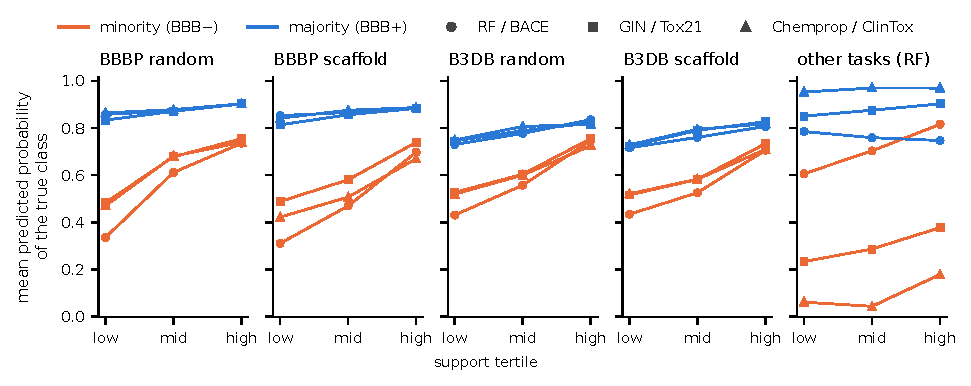
\includegraphics[width=\linewidth]{supp_mechanism.pdf}
\caption{\textbf{Mean predicted probability of the true class by support tertile} for minority (orange) and majority (blue) test compounds under each backbone (markers), LAC, CE, 20 splits. Right: random forest on the additional tasks (circles BACE, squares Tox21 SR-ARE, triangles ClinTox, random splits). The minority curve falls more steeply than the majority curve in every BBB cell; on Tox21 SR-ARE it also falls, yet the coverage gap is reversed (Proposition~\ref{prop:S-shared}(c)).}\label{fig:mech}
\end{figure}

\begin{figure}[h]\centering
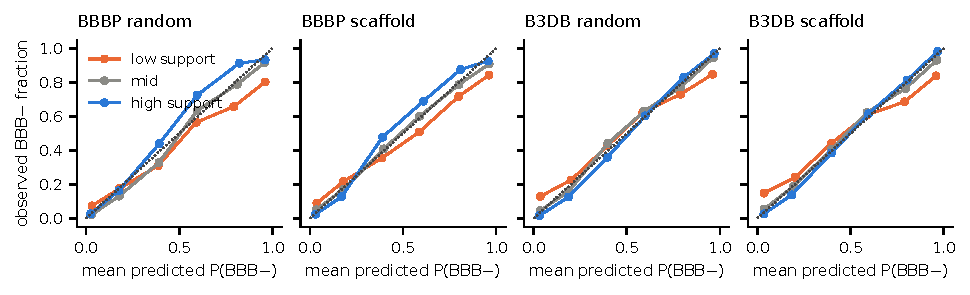
\includegraphics[width=\linewidth]{supp_reliability.pdf}
\caption{\textbf{Reliability by support tertile.} Observed BBB$-$ fraction against mean predicted BBB$-$ probability in fixed probability bins (at least 30 test appearances per point), pooled over backbones and 20 splits. On B3DB, low-support compounds (orange) are BBB$-$ more often than predicted at low predicted probability; on BBBP the pattern is inconsistent, as the support coefficient indicates.}\label{fig:rel}
\end{figure}

\textbf{Continuous support.} Over all BBB$-$ test appearances, the logistic slope of class-conditional coverage on maximal Tanimoto support is \V{sc.mond.slope.min}--\V{sc.mond.slope.max} log-odds per 0.1, with a split-bootstrap interval above zero in \V{sc.mond.npos} of 12 cells; under class $\times$ support it is \V{sc.mx.slope.min} to \V{sc.mx.slope.max} and its interval includes zero in most cells (Fig.~\ref{fig:curve}).

\begin{figure}[h]\centering
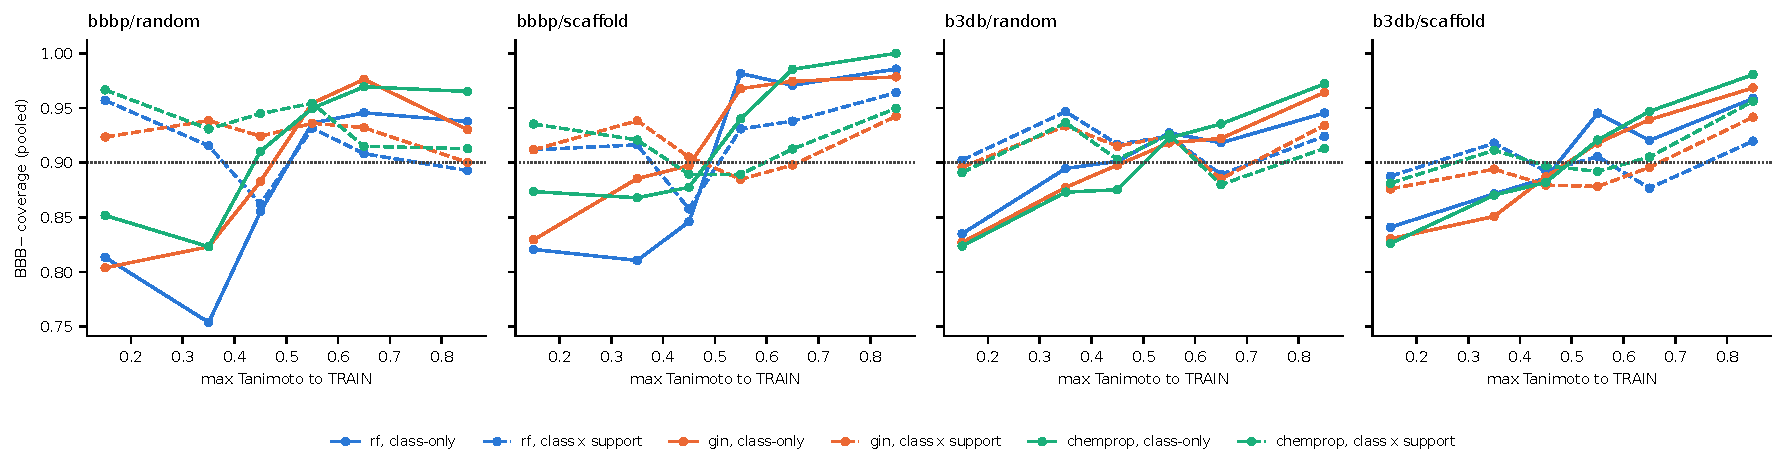
\includegraphics[width=\linewidth]{supp_support_curve.pdf}
\caption{\textbf{BBB$-$ coverage as a function of maximal Tanimoto support} (LAC, $\alpha=0.1$, CE), pooled over 20 splits in fixed support bins with at least 20 appearances. Solid: class-conditional; dashed: class $\times$ support. Pooled intervals are optimistic because molecules recur across splits; inference uses the split bootstrap of the slope.}\label{fig:curve}
\end{figure}

\textbf{Calibration at a fixed score.} A logistic regression of the BBB$-$ label on the logit of the predicted BBB$-$ probability and support gives a support coefficient of \V{scal.b3db.coef.min} to \V{scal.b3db.coef.max} per 0.1 Tanimoto on B3DB, with intervals below zero in \V{scal.b3db.nneg} of 6 cells, and \V{scal.bbbp.coef.min} to \V{scal.bbbp.coef.max} on BBBP, where signs differ across backbones.

\textbf{Can calibration data alone flag the failure?} Leave-one-out coverage of BBB$-$ calibration molecules in the lowest support tertile, computed without test data, correlates weakly with test low-support coverage across the \V{ca.nsplits} splits (Spearman \V{ca.rho}); as a per-split flag at 0.85 it has sensitivity \V{ca.sens} and specificity \V{ca.spec}. Aggregated over splits, the calibration-only flag agrees with the test outcome in \V{ca.cellagree} of 12 cells, and the sign of the high-minus-low gap agrees in a fraction \V{ca.signagree} of splits. Calibration data can therefore support an audit across repeated splits but not a decision for a single deployment (Fig.~\ref{fig:calaudit}).

\begin{figure}[h]\centering
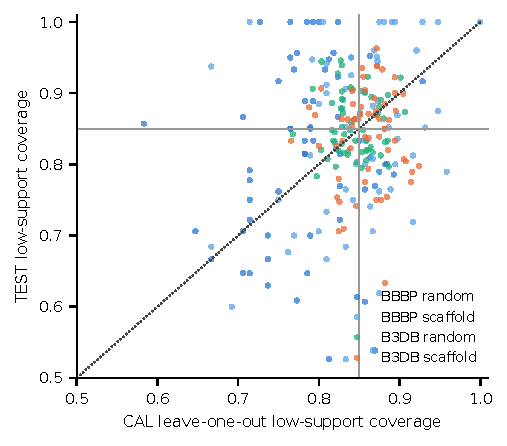
\includegraphics[width=0.5\linewidth]{supp_cal_audit.pdf}
\caption{\textbf{Calibration-only audit.} Leave-one-out coverage of low-support BBB$-$ calibration molecules against test low-support coverage, one point per split and backbone (240 points). Grey lines: flag threshold 0.85.}\label{fig:calaudit}
\end{figure}

% =====================================================================
\section{Other tasks and the prior protocol (exploratory)}\label{sec:general}
The same pipeline (random forest, CE, VAL tertile edges, seeds 100--119) was run on BACE, ClinTox and Tox21 SR-ARE from MoleculeNet~\cite{wu2018moleculenet}, with the minority label read from each dataset, and the random forest and graph convolutional network of Tursunbadalov and Tursunbadalov~\cite{tursunbadalov2026quiet} were rerun on their BBBP protocol (all parseable records, random 50/25/25 split, no VAL, so tertile edges come from CAL). Holm correction is applied within each block.

\begin{table}[h]\centering\scriptsize
\caption{\textbf{Other imbalanced tasks and the prior BBBP protocol.} Minority coverage (LAC, $\alpha=0.1$, CE; mean over 20 splits); $n^{\mathrm{min}}_{\mathrm{cal}}$: minority calibration molecules per split; last two columns: paired gain of class $\times$ support over class-conditional calibration in low-support minority coverage, seed bootstrap interval and Holm $p$ within the block. ClinTox cells are dominated by infinite thresholds and are not interpretable.}\label{tab:general}
\resizebox{\linewidth}{!}{% GENERATED by scripts/make_supplement_tables.py
\begin{tabular}{llcccccccc}
\toprule
Task & Model & $n^{\mathrm{min}}_{\mathrm{cal}}$ & Marg.\ class & Mond.\ class & Mond.\ low & Mond.\ high & C$\times$S low & C$\times$S $-$ Mond., low & Holm $p$\\
\midrule
BACE random & RF & 99.3 & 0.91 & 0.91 & 0.85 & 0.94 & 0.93 & +0.081 [0.045, 0.120] & 0.004\\
BACE scaffold & RF & 94.7 & 0.88 & 0.88 & 0.82 & 0.90 & 0.90 & +0.081 [0.044, 0.122] & 0.016\\
ClinTox random & RF & 8.5 & 0.00 & 0.97 & 0.98 & 0.94 & 1.00 & +0.023 [0.000, 0.057] & 0.849\\
ClinTox scaffold & RF & 8.3 & 0.00 & 0.99 & 0.98 & 1.00 & 1.00 & +0.020 [0.000, 0.050] & 0.849\\
Tox21 SR-ARE random & RF & 132.0 & 0.36 & 0.90 & 0.92 & 0.87 & 0.90 & -0.013 [-0.031, 0.003] & 0.686\\
Tox21 SR-ARE scaffold & RF & 148.3 & 0.46 & 0.91 & 0.93 & 0.87 & 0.91 & -0.017 [-0.036, 0.000] & 0.679\\
\midrule
BBBP random 50/25/25 & RF & 119.2 & 0.61 & 0.90 & 0.82 & 0.93 & 0.91 & +0.091 [0.048, 0.135] & $<$0.001\\
BBBP random 50/25/25 & GCN & 119.2 & 0.64 & 0.91 & 0.81 & 0.95 & 0.91 & +0.095 [0.071, 0.120] & $<$0.001\\
\bottomrule
\end{tabular}
}
\end{table}

\begin{figure}[h]\centering
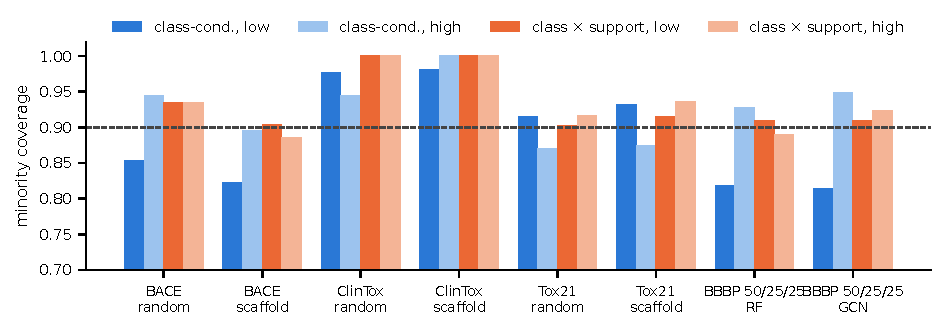
\includegraphics[width=\linewidth]{supp_generality.pdf}
\caption{\textbf{Low- and high-support minority coverage on other tasks and under the prior BBBP protocol} (LAC, $\alpha=0.1$, CE, 20 splits). BACE and the prior protocol show the BBB pattern (low below high under class-conditional calibration, levelled by class $\times$ support); Tox21 SR-ARE shows the reverse; ClinTox is dominated by infinite thresholds.}\label{fig:gen}
\end{figure}

% =====================================================================
\section{Persistent failures}\label{sec:persist}
\textbf{Definitions} are given in the main text (Section~5). Table~\ref{tab:plist} lists every cross-architecture persistent failure under the strict definition, Fig.~\ref{fig:struct} shows their structures, and Table~\ref{tab:pdesc} gives descriptor contrasts under both definitions.

\textbf{Curation findings.} Record numbers refer to the \texttt{NO.} column of the B3DB classification file; identifiers in brackets are those used in our code. (i) Record 3838 [B3DB:2544], labelled BBB$-$ (references R16, R10), is named rifampin but its SMILES encodes an unrelated difluoropyridine amide (PubChem CID 105381226); rifampin itself appears in records 1981, 5510 and 7390. (ii) Record 5692 [B3DB:3330], labelled BBB$-$ from a single reference (R23), is named phenylbutazone but drawn with a propyl chain; record 279, the correctly drawn butyl compound, is labelled BBB$+$ (logBB $-0.5$, 25 references). (iii) Record 5253 [B3DB:3001], cyclobenzaprine hydrochloride, labelled BBB$-$ from a single reference (R14), is drawn in a non-aromatic form that does not de-duplicate against record 1009, cyclobenzaprine, labelled BBB$+$ (logBB 1.06, three references); cyclobenzaprine is a centrally acting muscle relaxant. These are structural or record-level errors that can be checked from the file; they are distinct from disagreements between datasets about a correctly drawn compound, for which we do not decide which label is right.

\textbf{Name-level screen.} \V{nc.nconflict.min}--\V{nc.nconflict.max} eligible BBB$-$ molecules per B3DB setting share a normalized compound name with a BBB$+$ record of the raw file. Among strict failures this holds for \V{nc.b3db/random.strict.nfail} (random) and \V{nc.b3db/scaffold.strict.nfail} (scaffold), \V{nc.b3db/random.strict.ratefail}\% and \V{nc.b3db/scaffold.strict.ratefail}\% against \V{nc.b3db/random.strict.raterest}\% and \V{nc.b3db/scaffold.strict.raterest}\% of other eligible molecules (Fisher $p=\V{nc.b3db/random.strict.p}$ and \V{nc.b3db/scaffold.strict.p}); under the majority rule \V{nc.b3db/random.majority.ratefail}\% and \V{nc.b3db/scaffold.majority.ratefail}\% ($p=\V{nc.b3db/random.majority.p}$, \V{nc.b3db/scaffold.majority.p}). Names are an imperfect key in both directions: in the raw B3DB file some compound names are attached to unrelated structures (for example, records named dihydroergotamine, polythiazide and demeclocycline), so a same-name match can join different compounds. This is therefore a screen rather than a verdict on any label. The names given for shared failures in Table~\ref{tab:plist} were checked against their structures; only the rifampin record is mismatched, and it is flagged.

\textbf{Label audit.} Of \V{la.nshared} BBBP molecules found in B3DB by connectivity key (\V{la.overlap}\%), \V{la.ndis} carry different labels (\V{la.negpos} BBB$-$ in BBBP and BBB$+$ in B3DB; \V{la.posneg} the reverse). Among eligible BBBP test molecules that occur in B3DB, the majority-rule failure rate is higher for label conflicts on random splits (\V{la.bbbp/random.majority.fdis} of \V{la.bbbp/random.majority.ndis}; odds ratio \V{la.bbbp/random.majority.or}, Fisher $p=\V{la.bbbp/random.majority.p}$) and scaffold splits (\V{la.bbbp/scaffold.majority.fdis} of \V{la.bbbp/scaffold.majority.ndis}; \V{la.bbbp/scaffold.majority.or}, $p=\V{la.bbbp/scaffold.majority.p}$). None of the \V{la.b3db/random.majority.ndis} conflicting B3DB molecules is a failure.

\textbf{Sensitivity without the three records.} Removing the three records from calibration and test and recomputing all thresholds gives \V{pfx.b3db/random.n_cross_arch} cross-architecture failures on B3DB random (null mean \V{pfx.b3db/random.null}) and \V{pfx.b3db/scaffold.n_cross_arch} on B3DB scaffold (null mean \V{pfx.b3db/scaffold.null}), compared with \V{pf.b3db/random.n_cross_arch} and \V{pf.b3db/scaffold.n_cross_arch} in the primary analysis; BBBP results are unaffected. The concordance conclusion is unchanged.

\textbf{Concordance and appearance counts.} Table~\ref{tab:conc} compares the observed number of strict cross-architecture failures with the primary null (each backbone's persistence indicator permuted within strata of the number of appearances $k$) and with a covariate-stratified null that also permutes within support and TPSA tertiles, which absorbs agreement explained by those covariates. It also gives the distribution of $k$: a strict failure tested twice is weaker evidence than one tested five times.

\begin{table}[h]\centering\scriptsize
\caption{\textbf{Cross-architecture concordance against two nulls} (10{,}000 permutations each) and appearance counts of strict failures. null$_k$: strata of $k$ (capped at 6); null$_{\mathrm{cov}}$: strata of $k\times$ support tertile $\times$ TPSA tertile.}\label{tab:conc}
\resizebox{\linewidth}{!}{% GENERATED by scripts/make_supplement_tables.py
\begin{tabular}{lrrcccccrr}
\toprule
Setting & eligible & strict & null$_k$ & $p_k$ & null$_{\mathrm{cov}}$ & $p_{\mathrm{cov}}$ & $k$: median (range) & $k\ge3$ & $k\ge4$\\
\midrule
B3DB random & 1149 & 10 & 0.09 & $<$0.001 & 0.77 & $<$0.001 & 3 (2--5) & 8 & 1\\
B3DB scaffold & 1199 & 14 & 0.23 & $<$0.001 & 0.83 & $<$0.001 & 2 (2--5) & 6 & 3\\
BBBP random & 368 & 2 & 0.02 & $<$0.001 & 0.32 & 0.018 & 4 (3--6) & 2 & 1\\
BBBP scaffold & 386 & 1 & 0.02 & 0.020 & 0.12 & 0.120 & 2 (2--2) & 0 & 0\\
BBBP$\to$B3DB & 1070 & 0 & 0.01 & 1.000 & 0.03 & 1.000 & -- & 0 & 0\\
\bottomrule
\end{tabular}
}
\end{table}

\begin{table}[h]\centering\scriptsize
\caption{\textbf{Cross-architecture persistent BBB$-$ failures} (strict definition). $k$: number of splits in which the molecule was tested; support: mean maximal Tanimoto similarity to TRAIN; flag: label in the other dataset or curation finding.}\label{tab:plist}
\resizebox{\linewidth}{!}{% GENERATED by scripts/make_supplement_tables.py
\begin{tabular}{llrrrrrrl}
\toprule
Setting & Compound & $k$ & TPSA & HBD & MW & cLogP & support & flag\\
\midrule
B3DB random & naftifine & 5 & 3.2 & 0 & 287 & 4.99 & 0.53 & \\
B3DB random & cyclobenzaprine hydrochloride & 3 & 3.2 & 0 & 275 & 2.64 & 0.54 & curation error (mis-drawn)\\
B3DB random & desloratadine & 2 & 24.9 & 1 & 311 & 4.02 & 0.43 & \\
B3DB random & bromhexine & 3 & 29.3 & 1 & 376 & 4.56 & 0.29 & \\
B3DB random & cytisine & 3 & 34.0 & 1 & 190 & 0.55 & 0.61 & \\
B3DB random & menadione & 3 & 34.1 & 0 & 172 & 2.01 & 0.29 & \\
B3DB random & dapiprazole & 3 & 37.2 & 0 & 325 & 2.29 & 0.40 & \\
B3DB random & B3DB:2805 & 3 & 39.1 & 1 & 255 & 2.53 & 0.29 & \\
B3DB random & emetine hydrochloride & 3 & 52.2 & 1 & 481 & 4.94 & 0.45 & \\
B3DB random & troxipide & 2 & 68.8 & 2 & 294 & 1.19 & 0.39 & \\
B3DB scaffold & cyclobenzaprine hydrochloride & 4 & 3.2 & 0 & 275 & 2.64 & 0.52 & curation error (mis-drawn)\\
B3DB scaffold & naftifine & 3 & 3.2 & 0 & 287 & 4.99 & 0.40 & \\
B3DB scaffold & ticlopidine hydrochloride & 3 & 3.2 & 0 & 264 & 3.96 & 0.29 & \\
B3DB scaffold & desloratadine & 2 & 24.9 & 1 & 311 & 4.02 & 0.29 & \\
B3DB scaffold & diethylcarbamazine citrate & 2 & 26.8 & 0 & 199 & 0.70 & 0.35 & \\
B3DB scaffold & rifampin & 2 & 33.2 & 0 & 288 & 3.20 & 0.28 & curation error (name/structure)\\
B3DB scaffold & B3DB:13 & 2 & 36.4 & 2 & 161 & 1.06 & 0.45 & \\
B3DB scaffold & dapiprazole & 5 & 37.2 & 0 & 325 & 2.29 & 0.41 & \\
B3DB scaffold & B3DB:2805 & 3 & 39.1 & 1 & 255 & 2.53 & 0.27 & \\
B3DB scaffold & phenylbutazone & 2 & 40.6 & 0 & 294 & 3.40 & 0.44 & curation error (mis-drawn)\\
B3DB scaffold & dropropizine & 2 & 46.9 & 2 & 236 & 0.16 & 0.39 & \\
B3DB scaffold & acetohydroxamic acid & 2 & 49.3 & 2 & 75 & -0.49 & 0.43 & \\
B3DB scaffold & emetine hydrochloride & 2 & 52.2 & 1 & 481 & 4.94 & 0.46 & \\
B3DB scaffold & diazoxide & 4 & 58.5 & 1 & 231 & 1.68 & 0.32 & \\
BBBP random & Phenylbutazone & 3 & 40.6 & 0 & 308 & 3.79 & 0.35 & B3DB: BBB$+$\\
BBBP random & Thiopental & 6 & 58.2 & 2 & 242 & 1.35 & 0.73 & B3DB: BBB$+$\\
BBBP scaffold & Phenylbutazone & 2 & 40.6 & 0 & 308 & 3.79 & 0.35 & B3DB: BBB$+$\\
\bottomrule
\end{tabular}
}
\end{table}

\begin{figure}[h]\centering
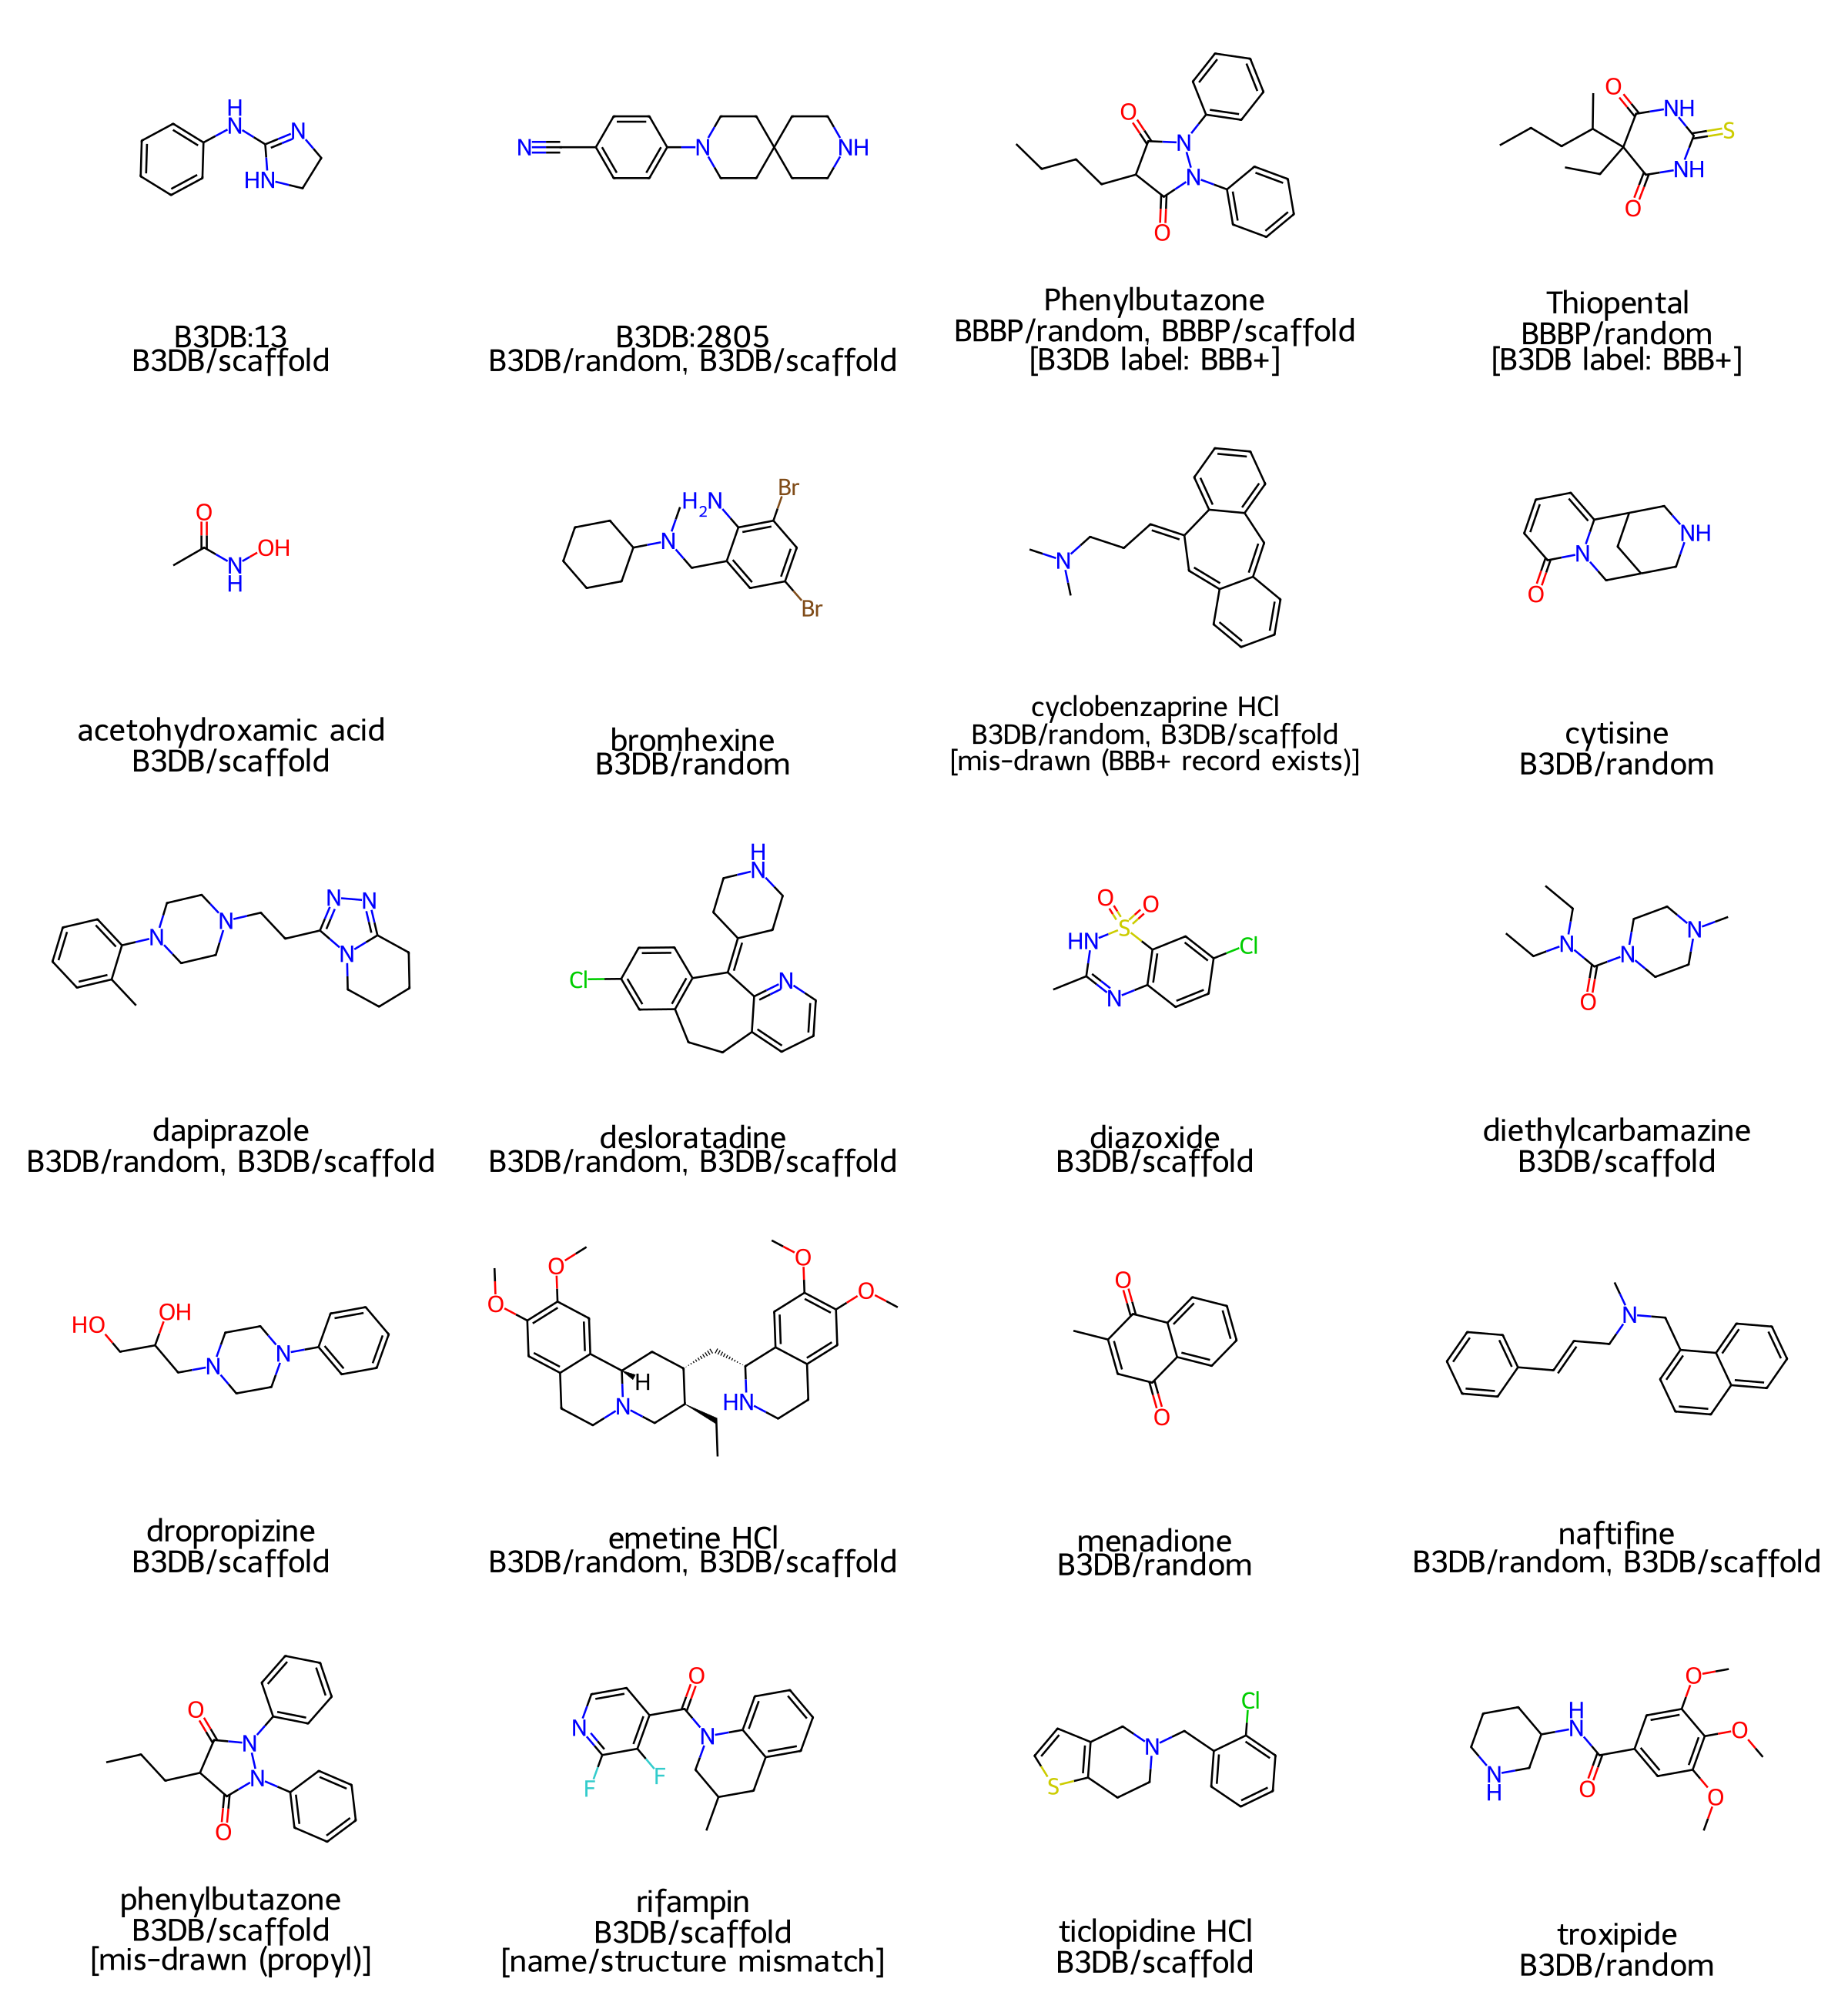
\includegraphics[width=\linewidth]{supp_persistent_structures.png}
\caption{\textbf{Structures of cross-architecture persistent BBB$-$ failures} (unique molecules, strict definition), with the settings in which each is persistent and dataset flags.}\label{fig:struct}
\end{figure}

\begin{table}[h]\centering\scriptsize
\caption{\textbf{Descriptor contrasts}, persistent versus other eligible BBB$-$ molecules (unique molecules). AUC: probability that a persistent molecule has the larger value. Holm over the four primary descriptors and the settings tested within each definition; tests require at least five molecules per group. Support is descriptive.}\label{tab:pdesc}
\resizebox{\linewidth}{!}{% GENERATED by scripts/make_supplement_tables.py
\begin{tabular}{lllcrrcc}
\toprule
Definition & Setting & Descriptor & $n$ pers./rest & median pers. & median rest & AUC & Holm\\
\midrule
strict & B3DB random & TPSA & 10 / 1139 & 34.09 & 92.79 & 0.09 & $<$0.001\\
strict & B3DB random & HBD & 10 / 1139 & 1.00 & 2.00 & 0.19 & 0.002\\
strict & B3DB random & MW & 10 / 1139 & 290.88 & 380.49 & 0.28 & 0.044\\
strict & B3DB random & cLogP & 10 / 1139 & 2.59 & 2.12 & 0.62 & 0.352\\
strict & B3DB random & support & 10 / 1139 & 0.41 & 0.53 & 0.32 & --\\
strict & B3DB scaffold & TPSA & 14 / 1185 & 36.81 & 93.06 & 0.09 & $<$0.001\\
strict & B3DB scaffold & HBD & 14 / 1185 & 0.50 & 2.00 & 0.19 & $<$0.001\\
strict & B3DB scaffold & MW & 14 / 1185 & 269.59 & 384.65 & 0.20 & $<$0.001\\
strict & B3DB scaffold & cLogP & 14 / 1185 & 2.59 & 2.12 & 0.56 & 0.444\\
strict & B3DB scaffold & support & 14 / 1185 & 0.39 & 0.44 & 0.37 & --\\
strict & BBBP random & TPSA & 2 / 366 & 49.41 & 111.92 & -- & --\\
strict & BBBP random & HBD & 2 / 366 & 1.00 & 3.00 & -- & --\\
strict & BBBP random & MW & 2 / 366 & 275.36 & 400.50 & -- & --\\
strict & BBBP random & cLogP & 2 / 366 & 2.57 & 1.22 & -- & --\\
strict & BBBP random & support & 2 / 366 & 0.54 & 0.59 & -- & --\\
strict & BBBP scaffold & TPSA & 1 / 385 & 40.62 & 110.43 & -- & --\\
strict & BBBP scaffold & HBD & 1 / 385 & 0.00 & 3.00 & -- & --\\
strict & BBBP scaffold & MW & 1 / 385 & 308.38 & 403.83 & -- & --\\
strict & BBBP scaffold & cLogP & 1 / 385 & 3.79 & 1.37 & -- & --\\
strict & BBBP scaffold & support & 1 / 385 & 0.35 & 0.46 & -- & --\\
strict & BBBP$\to$B3DB & TPSA & 0 / 1070 & -- & 87.34 & -- & --\\
strict & BBBP$\to$B3DB & HBD & 0 / 1070 & -- & 2.00 & -- & --\\
strict & BBBP$\to$B3DB & MW & 0 / 1070 & -- & 366.44 & -- & --\\
strict & BBBP$\to$B3DB & cLogP & 0 / 1070 & -- & 2.47 & -- & --\\
strict & BBBP$\to$B3DB & support & 0 / 1070 & -- & 0.32 & -- & --\\
\midrule
majority & B3DB random & TPSA & 42 / 1107 & 36.78 & 94.83 & 0.14 & $<$0.001\\
majority & B3DB random & HBD & 42 / 1107 & 1.00 & 2.00 & 0.22 & $<$0.001\\
majority & B3DB random & MW & 42 / 1107 & 287.92 & 383.52 & 0.26 & $<$0.001\\
majority & B3DB random & cLogP & 42 / 1107 & 2.65 & 2.11 & 0.58 & 0.286\\
majority & B3DB random & support & 42 / 1107 & 0.37 & 0.54 & 0.33 & --\\
majority & B3DB scaffold & TPSA & 55 / 1144 & 36.42 & 95.94 & 0.13 & $<$0.001\\
majority & B3DB scaffold & HBD & 55 / 1144 & 1.00 & 2.00 & 0.21 & $<$0.001\\
majority & B3DB scaffold & MW & 55 / 1144 & 288.44 & 389.64 & 0.26 & $<$0.001\\
majority & B3DB scaffold & cLogP & 55 / 1144 & 2.92 & 2.11 & 0.60 & 0.083\\
majority & B3DB scaffold & support & 55 / 1144 & 0.32 & 0.44 & 0.30 & --\\
majority & BBBP random & TPSA & 14 / 354 & 69.28 & 112.73 & 0.24 & 0.010\\
majority & BBBP random & HBD & 14 / 354 & 2.00 & 3.00 & 0.27 & 0.027\\
majority & BBBP random & MW & 14 / 354 & 313.12 & 404.63 & 0.37 & 0.286\\
majority & BBBP random & cLogP & 14 / 354 & 3.04 & 1.11 & 0.73 & 0.027\\
majority & BBBP random & support & 14 / 354 & 0.44 & 0.59 & 0.38 & --\\
majority & BBBP scaffold & TPSA & 12 / 374 & 63.89 & 111.90 & 0.22 & 0.010\\
majority & BBBP scaffold & HBD & 12 / 374 & 2.00 & 3.00 & 0.22 & 0.009\\
majority & BBBP scaffold & MW & 12 / 374 & 359.32 & 405.49 & 0.35 & 0.286\\
majority & BBBP scaffold & cLogP & 12 / 374 & 2.87 & 1.33 & 0.70 & 0.092\\
majority & BBBP scaffold & support & 12 / 374 & 0.30 & 0.46 & 0.26 & --\\
majority & BBBP$\to$B3DB & TPSA & 46 / 1024 & 36.00 & 89.06 & 0.19 & $<$0.001\\
majority & BBBP$\to$B3DB & HBD & 46 / 1024 & 1.00 & 2.00 & 0.26 & $<$0.001\\
majority & BBBP$\to$B3DB & MW & 46 / 1024 & 287.92 & 371.32 & 0.31 & $<$0.001\\
majority & BBBP$\to$B3DB & cLogP & 46 / 1024 & 2.80 & 2.44 & 0.56 & 0.286\\
majority & BBBP$\to$B3DB & support & 46 / 1024 & 0.31 & 0.32 & 0.49 & --\\
\bottomrule
\end{tabular}
}
\end{table}

\begin{figure}[h]\centering
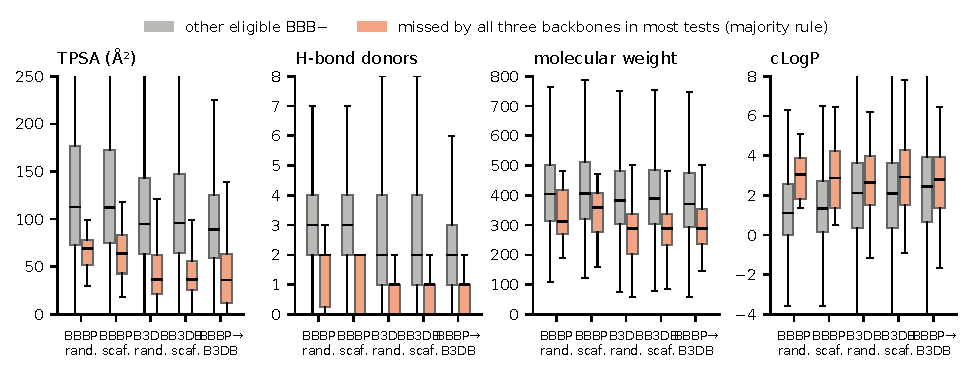
\includegraphics[width=\linewidth]{supp_descriptors.pdf}
\caption{\textbf{Descriptors of shared failures} (majority rule, which populates all five settings) against other eligible BBB$-$ molecules; unique molecules, boxes show quartiles. Holm-adjusted tests are in Table~\ref{tab:pdesc}.}\label{fig:desc}
\end{figure}

\begin{table}[h]\centering\scriptsize
\caption{\textbf{TPSA association with being missed, adjusted for support.} Logistic regression of a miss under class-conditional calibration on standardized descriptors over all BBB$-$ test appearances; coefficient and 95\% interval from 400 bootstrap resamples of splits. Permutation $p$: TPSA permuted within support tertiles (500 permutations).}\label{tab:adj}
\resizebox{\linewidth}{!}{% GENERATED by scripts/make_supplement_tables.py
\begin{tabular}{llcccc}
\toprule
Model & Setting & TPSA, unadjusted & + support & + support, MW, cLogP & permutation $p$\\
\midrule
RF & BBBP random & -3.07 [-3.56, -2.67] & -2.85 [-3.32, -2.46] & -2.78 [-3.89, -1.83] & $<$0.002\\
RF & BBBP scaffold & -2.86 [-3.90, -1.92] & -2.44 [-3.52, -1.33] & -0.80 [-2.19, 0.41] & $<$0.002\\
RF & B3DB random & -2.12 [-2.69, -1.63] & -2.12 [-2.67, -1.63] & -2.23 [-2.98, -1.41] & $<$0.002\\
RF & B3DB scaffold & -2.11 [-2.59, -1.62] & -2.04 [-2.50, -1.58] & -2.90 [-3.55, -2.21] & $<$0.002\\
GIN & BBBP random & -1.54 [-1.98, -1.14] & -1.36 [-1.86, -0.97] & -3.00 [-3.83, -2.05] & $<$0.002\\
GIN & BBBP scaffold & -0.89 [-1.74, -0.20] & -0.46 [-1.20, 0.13] & -1.22 [-2.89, 0.50] & $<$0.002\\
GIN & B3DB random & -1.13 [-1.44, -0.87] & -1.03 [-1.32, -0.71] & -1.82 [-2.31, -1.42] & $<$0.002\\
GIN & B3DB scaffold & -1.21 [-1.62, -0.80] & -1.11 [-1.54, -0.72] & -2.76 [-3.34, -2.24] & $<$0.002\\
Chemprop & BBBP random & -1.73 [-2.19, -1.30] & -1.49 [-2.02, -1.04] & -2.65 [-3.83, -1.61] & $<$0.002\\
Chemprop & BBBP scaffold & -2.01 [-2.86, -1.41] & -1.63 [-2.56, -0.96] & -0.85 [-1.77, 0.11] & $<$0.002\\
Chemprop & B3DB random & -1.61 [-1.98, -1.27] & -1.50 [-1.84, -1.15] & -1.91 [-2.57, -1.27] & $<$0.002\\
Chemprop & B3DB scaffold & -1.57 [-1.97, -1.14] & -1.43 [-1.83, -1.04] & -2.44 [-3.00, -1.76] & $<$0.002\\
\bottomrule
\end{tabular}
}
\end{table}

\begin{figure}[h]\centering
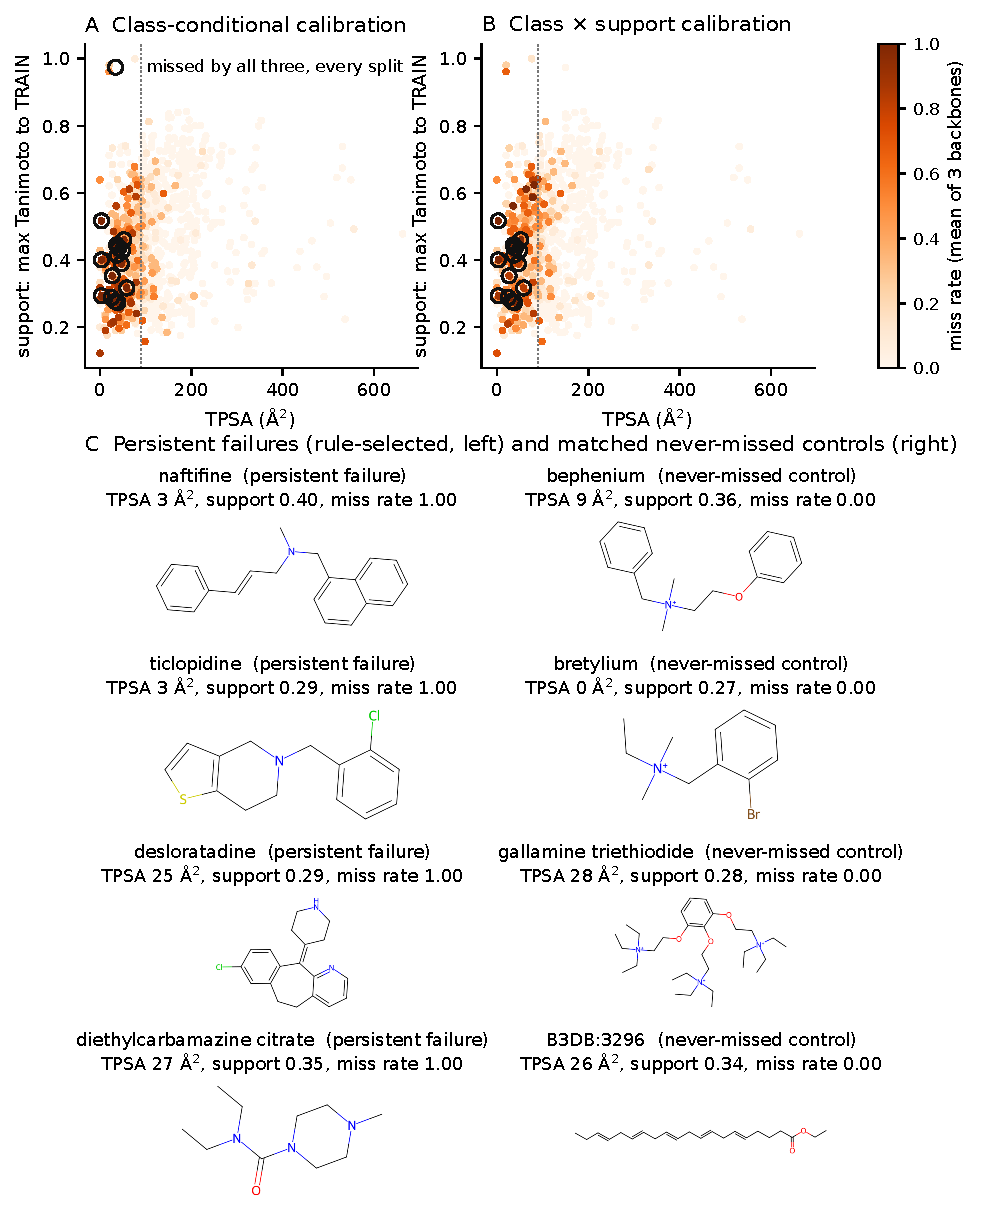
\includegraphics[width=\linewidth]{fig_chemistry_b3db_scaffold.pdf}
\caption{\textbf{Chemistry of the misses, B3DB scaffold splits.} (A, B) Every eligible BBB$-$ test molecule by TPSA and mean support, coloured by its miss rate (mean over the three backbones) under class-conditional (A) and class $\times$ support (B) calibration; circles: strict cross-architecture failures. (C) Strict failures selected by a fixed rule (lowest TPSA first, the three curation-error records excluded), each with the never-missed BBB$-$ molecule nearest in TPSA and support. Several controls are permanently charged; we did not test this pattern on independent data and report it only as a hypothesis.}\label{fig:chem}
\end{figure}

% =====================================================================
\section{Screening decisions}\label{sec:screen}
\begin{table}[h]\centering\scriptsize
\caption{\textbf{Decision metrics at $\alpha=0.1$}, mean over three backbones and 20 splits. Rejection baselines are matched per split to the deferral rate of class $\times$ support (C$\times$S); in the VAL-threshold variants the deferral rate and the rejection thresholds are set on VAL, so they are not matched on the test set.}\label{tab:screen}
\resizebox{\linewidth}{!}{% GENERATED by scripts/make_supplement_tables.py
\begin{tabular}{llcccc}
\toprule
Setting & Rule & deferral & accepted error & BBB$-$ accepted as BBB$+$ & low-support accepted error\\
\midrule
BBBP random & marginal & 0.067 & 0.101 & 0.286 & 0.147\\
 & Mondrian & 0.210 & 0.128 & 0.089 & 0.199\\
 & C$\times$S & 0.306 & 0.125 & 0.069 & 0.225\\
 & AD rejection & 0.306 & 0.102 & 0.194 & 0.150\\
 & conf.\ rejection & 0.306 & 0.057 & 0.126 & 0.094\\
 & AD rejection, VAL threshold & 0.310 & 0.101 & 0.192 & 0.157\\
 & conf.\ rejection, VAL threshold & 0.322 & 0.055 & 0.120 & 0.090\\
\midrule
BBBP scaffold & marginal & 0.139 & 0.115 & 0.322 & 0.167\\
 & Mondrian & 0.311 & 0.160 & 0.095 & 0.241\\
 & C$\times$S & 0.383 & 0.155 & 0.076 & 0.196\\
 & AD rejection & 0.383 & 0.124 & 0.216 & 0.099\\
 & conf.\ rejection & 0.383 & 0.070 & 0.146 & 0.113\\
 & AD rejection, VAL threshold & 0.421 & 0.122 & 0.196 & 0.085\\
 & conf.\ rejection, VAL threshold & 0.409 & 0.067 & 0.139 & 0.109\\
\midrule
B3DB random & marginal & 0.270 & 0.131 & 0.194 & 0.209\\
 & Mondrian & 0.303 & 0.137 & 0.094 & 0.210\\
 & C$\times$S & 0.322 & 0.134 & 0.086 & 0.185\\
 & AD rejection & 0.322 & 0.172 & 0.205 & 0.232\\
 & conf.\ rejection & 0.322 & 0.116 & 0.160 & 0.194\\
 & AD rejection, VAL threshold & 0.325 & 0.172 & 0.205 & 0.240\\
 & conf.\ rejection, VAL threshold & 0.323 & 0.116 & 0.160 & 0.193\\
\midrule
B3DB scaffold & marginal & 0.291 & 0.145 & 0.203 & 0.234\\
 & Mondrian & 0.317 & 0.152 & 0.110 & 0.243\\
 & C$\times$S & 0.340 & 0.150 & 0.102 & 0.221\\
 & AD rejection & 0.340 & 0.185 & 0.208 & 0.249\\
 & conf.\ rejection & 0.340 & 0.132 & 0.174 & 0.220\\
 & AD rejection, VAL threshold & 0.357 & 0.184 & 0.202 & 0.222\\
 & conf.\ rejection, VAL threshold & 0.345 & 0.130 & 0.173 & 0.218\\
\midrule
BBBP$\to$B3DB & marginal & 0.234 & 0.378 & 0.532 & 0.454\\
 & Mondrian & 0.378 & 0.319 & 0.186 & 0.393\\
 & C$\times$S & 0.495 & 0.297 & 0.127 & 0.371\\
 & AD rejection & 0.495 & 0.339 & 0.295 & 0.421\\
 & conf.\ rejection & 0.495 & 0.336 & 0.321 & 0.426\\
 & AD rejection, VAL threshold & 0.647 & 0.298 & 0.179 & 0.401\\
 & conf.\ rejection, VAL threshold & 0.599 & 0.317 & 0.244 & 0.416\\
\bottomrule
\end{tabular}
}
\end{table}

\begin{table}[h]\centering\scriptsize
\caption{\textbf{Class-conditional calibration plus a rejection filter} at $\alpha=0.1$, mean over three backbones and 20 splits. The filter defers, among the singleton calls of class-conditional calibration, the compounds with the lowest support (AD) or confidence until total deferral equals that of class $\times$ support on the same split (matched without test labels); VAL rows set the extra deferral and the cut-off on VAL. Where class-conditional calibration already defers more, no extra deferral is added.}\label{tab:calrej}
\resizebox{\linewidth}{!}{% GENERATED by scripts/make_supplement_tables.py
\begin{tabular}{llccc}
\toprule
Setting & Rule & deferral & accepted error & BBB$-$ accepted as BBB$+$\\
\midrule
BBBP random & C$\times$S & 0.306 & 0.125 & 0.069\\
 & Mondrian & 0.210 & 0.128 & 0.089\\
 & Mondrian + AD filter & 0.312 & 0.113 & 0.062\\
 & Mondrian + conf.\ filter & 0.312 & 0.085 & 0.083\\
 & Mondrian + AD filter, VAL & 0.309 & 0.112 & 0.062\\
 & Mondrian + conf.\ filter, VAL & 0.315 & 0.083 & 0.082\\
\midrule
BBBP scaffold & C$\times$S & 0.383 & 0.155 & 0.076\\
 & Mondrian & 0.311 & 0.160 & 0.095\\
 & Mondrian + AD filter & 0.394 & 0.145 & 0.073\\
 & Mondrian + conf.\ filter & 0.394 & 0.124 & 0.089\\
 & Mondrian + AD filter, VAL & 0.410 & 0.142 & 0.066\\
 & Mondrian + conf.\ filter, VAL & 0.412 & 0.115 & 0.089\\
\midrule
B3DB random & C$\times$S & 0.322 & 0.134 & 0.086\\
 & Mondrian & 0.303 & 0.137 & 0.094\\
 & Mondrian + AD filter & 0.326 & 0.132 & 0.085\\
 & Mondrian + conf.\ filter & 0.326 & 0.128 & 0.094\\
 & Mondrian + AD filter, VAL & 0.324 & 0.132 & 0.085\\
 & Mondrian + conf.\ filter, VAL & 0.327 & 0.128 & 0.094\\
\midrule
B3DB scaffold & C$\times$S & 0.340 & 0.150 & 0.102\\
 & Mondrian & 0.317 & 0.152 & 0.110\\
 & Mondrian + AD filter & 0.344 & 0.146 & 0.099\\
 & Mondrian + conf.\ filter & 0.344 & 0.142 & 0.110\\
 & Mondrian + AD filter, VAL & 0.347 & 0.145 & 0.098\\
 & Mondrian + conf.\ filter, VAL & 0.341 & 0.144 & 0.110\\
\midrule
BBBP$\to$B3DB & C$\times$S & 0.495 & 0.297 & 0.127\\
 & Mondrian & 0.378 & 0.319 & 0.186\\
 & Mondrian + AD filter & 0.497 & 0.295 & 0.133\\
 & Mondrian + conf.\ filter & 0.497 & 0.311 & 0.179\\
 & Mondrian + AD filter, VAL & 0.563 & 0.274 & 0.111\\
 & Mondrian + conf.\ filter, VAL & 0.553 & 0.305 & 0.172\\
\bottomrule
\end{tabular}
}
\end{table}

% =====================================================================
\section{Verification and reproducibility}\label{sec:verify}
Each number in the main text is a macro written by \path{scripts/make_paper_numbers.py} together with its source file, filter and aggregation (\path{generated/numbers_provenance.csv}). \path{scripts/verify_paper_numbers.py}, which imports only NumPy, pandas, SciPy and RDKit and shares no code with the analysis pipeline, recomputes each value from the cached predictions with its own conformal quantile, stratum assignment, count-based merging rule, Wilcoxon and Holm procedures and logistic fit, and records whether each value was recomputed exactly, replicated with independent random draws within a stated tolerance, or cross-checked against per-split outputs. Persistent-failure results are recomputed by \path{scripts/verify_persistent_failures.py}. The analysis reproduces the per-split coverages of the evaluation pipeline exactly before any per-molecule result is computed. Exploratory results that depend on the pipeline's own randomization (random strata) or on implementations of published methods are cross-checked against per-split outputs rather than recomputed. Counts that depend on whether a bootstrap interval excludes zero are replicated with independent draws and may differ by the number of cells whose interval endpoint lies within 0.02 of zero; such counts are not used as firm results. In a few small splits a support tertile contains no BBB$-$ test molecule; that split contributes no value for the tertile, identically in the analysis and in the verifier. All analyses of the cached predictions were reproduced on a second computing platform with identical results; models retrained there for the additional tasks gave identical splits but slightly different predictions (a different RDKit release), with unchanged conclusions. Package versions are pinned in \path{requirements-lock.txt}. All code, data and commands are available in the public repository listed in the main text.

\clearpage
\bibliographystyle{abbrvnat}
{\small\bibliography{references_final}}
\end{document}
